\documentclass{buthesis}

\usepackage{hologo}
\usepackage{booktabs}
\usepackage{float} 
\usepackage{hyphenat}
\usepackage{tabularx,array}
\usepackage{amsmath}
\usepackage{svg,graphicx}
\usepackage{tabularx, ragged2e}
\newcolumntype{Y}{>{\RaggedRight\arraybackslash}X}
\usepackage[utf8]{inputenc}
\usepackage{newunicodechar}
\usepackage[nottoc]{tocbibind}
\usepackage[titletoc]{appendix}
\setcounter{tocdepth}{2}
\usepackage{listings}
\usepackage{xcolor}
\usepackage[utf8]{inputenc}
\usepackage{listings}
\usepackage{listingsutf8}
\usepackage{import}


\svgsetup{
	inkscapeexe={C:/Program Files/Inkscape/bin/inkscape.exe},
	inkscapelatex=true,
	inkscapearea=page,
	clean=true
}


\lstset{
  inputencoding=utf8,
  basicstyle=\ttfamily\small,
  breaklines=true,
  literate=
    {–}{{-}}1 {—}{{---}}1 {…}{{\ldots}}1
    {→}{{$\to$}}1 {←}{{$\leftarrow$}}1 {⇒}{{$\Rightarrow$}}1
    {α}{{$\alpha$}}1 {β}{{$\beta$}}1 {γ}{{$\gamma$}}1 {δ}{{$\delta$}}1
    {π}{{$\pi$}}1 {σ}{{$\sigma$}}1 {τ}{{$\tau$}}1
    {Δ}{{$\Delta$}}1 {Σ}{{$\Sigma$}}1 {Ω}{{$\Omega$}}1
}

\lstset{
  basicstyle=\ttfamily\small,
  breaklines=true,
  breakatwhitespace=true,
  columns=fullflexible,
  keepspaces=true,
  tabsize=2,
  frame=single,
  rulecolor=\color{black!20},
  xleftmargin=0.5em, xrightmargin=0.5em,
  aboveskip=0.75\baselineskip, belowskip=0.75\baselineskip,
  postbreak=\mbox{\textellipsis\space}
}


\newunicodechar{π}{\ensuremath{\pi}}
\newunicodechar{α}{\ensuremath{\alpha}}
\newunicodechar{β}{\ensuremath{\beta}}
\newunicodechar{γ}{\ensuremath{\gamma}}
\newunicodechar{δ}{\ensuremath{\delta}}
\newunicodechar{ε}{\ensuremath{\varepsilon}}
\newunicodechar{θ}{\ensuremath{\theta}}
\newunicodechar{λ}{\ensuremath{\lambda}}
\newunicodechar{μ}{\ensuremath{\mu}}
\newunicodechar{ρ}{\ensuremath{\rho}}
\newunicodechar{σ}{\ensuremath{\sigma}}
\newunicodechar{τ}{\ensuremath{\tau}}
\newunicodechar{φ}{\ensuremath{\varphi}}
\newunicodechar{ω}{\ensuremath{\omega}}
\newunicodechar{Δ}{\ensuremath{\Delta}}
\newunicodechar{Λ}{\ensuremath{\Lambda}}
\newunicodechar{Σ}{\ensuremath{\Sigma}}
\newunicodechar{Ω}{\ensuremath{\Omega}}



\begin{document}

\title{Context-Driven Root Cause Analysis for Software Security Vulnerabilities}
\author{Md Iqbal Hossain Shuvo}

\beforepreface
\prefacesection{Abstract}

This work introduces a context-aware causal inference framework designed to enhance both interpretability and robustness in automated vulnerability detection. The proposed method explicitly reconstructs root-to-sink causal chains that trace the propagation of vulnerabilities across functions, thereby revealing inter-procedural spreading behaviors that conventional models overlook. Programs are encoded as heterogeneous graphs enriched with GraphCodeBERT representations, enabling a nuanced capture of syntactic and semantic dependencies. During inference, beam search with Adaptive Causal Contextualization (ACC) assembles executable causal chains that respect control- and data-flow reachability while maintaining cross-functional coherence and avoiding cycles. To further improve the interpretability of long, multi-function traces, a Causal Knowledge Graph (CKG) of frequently observed relation motifs is mined and employed as a weak structural prior, gently guiding beam expansion without compromising ACC’s admissibility.

To rigorously evaluate the causal soundness of the proposed framework, two novel metrics are introduced. The Counterfactual Consistency Score (CCS) quantifies the stability of predictions under targeted causal perturbations, while the Causal Feature Attribution Measure (CFAM) assesses the alignment between the model’s attention and the code elements that genuinely drive vulnerability outcomes. Together with traditional performance metrics, these measures establish a comprehensive evaluation protocol that validates both predictive effectiveness and causal grounding.

By transitioning from correlation-based analysis to mechanism-aware causal reasoning, this research advances the transparency, reliability, and practical utility of DL-based vulnerability analysis. The proposed framework not only enhances developers’ ability to interpret model outputs but also provides a principled foundation for trustworthy, traceable, and targeted remediation in real-world software systems.

\prefacesection{Acknowledgments}

I would like to express my sincere gratitude to everyone who contributed to the successful completion of this thesis. First, I thank my Supervisor, Y M, for their unwavering support, invaluable guidance, and patience throughout this research journey.

\figurespagetrue
\tablespagetrue

\afterpreface

%========================================
% Chapter 1 — Introduction
%========================================

\chapter{Introduction}
\label{chap:intro}

\section{Introduction}
Software now underpins critical infrastructure, financial services, scientific workflows, and everyday communication. As projects grow in size and heterogeneity, contemporary codebases span millions of lines and evolve under distributed development, increasing architectural complexity and the likelihood that subtle defects persist into production. When such defects are exploitable, they become security vulnerabilities that threaten confidentiality, integrity, and availability, with failures that may propagate across dependent components.

Traditional software assurance relies on two complementary approaches: static and dynamic analysis. Static analysis examines code without execution, employing rule-based systems, type reasoning, and data-flow frameworks to infer program behavior at scale. Dynamic analysis, in contrast, executes programs using real inputs or instrumented environments to observe actual runtime behavior. Each method has distinct advantages and limitations: static analysis provides broad coverage but often overestimates feasible execution paths, while dynamic analysis delivers precise traces at the expense of limited input coverage and scalability. When applied in isolation, neither approach consistently captures the holistic behavior of large, modular systems, particularly when data and control flows cross function or module boundaries via argument parameter mappings, return–caller relationships, aliasing, and nested control structures.

Machine learning or deep learning based methods have greatly improved traditional program analysis by using different structural representations of code, like sequences, trees, and graphs.  Graph-based models fit well with the structure of programs:  Abstract Syntax  Trees represent syntactic relationships, Control-Flow Graphs illustrate execution paths, and Data-Flow Graphs signify value dependencies; these perspectives can be amalgamated into cohesive representations like the Code Property Graph to facilitate integrated reasoning across syntactic, control, and data dimensions~\cite{yamaguchi2014cpg}.  Building on this foundation, models such as \emph{Devign} and subsequent graph neural network variants have achieved strong benchmark performance by fusing information from these complementary views~\cite{Zhou2019}, while post-hoc explainers like \emph{LEMNA} and \emph{GNNExplainer} identify key features or subgraphs to clarify model decisions~\cite{guo2018lemna,ying2019gnnexplainer}; structure-aware pretraining approaches such as \emph{GraphCodeBERT} enrich token embeddings with data-flow semantics to improve downstream performance~\cite{guo2021graphcodebert}.  Even with these improvements, many ML-based vulnerability detectors are still statement- or subgraph-centric. They focus on \emph{where} a flaw is likely to happen instead of \emph{how} it happens through the interaction of control and data flows. They also often rely on localized statistical patterns instead of clear causal relationships~\cite{Li2022Empirical,yang2022natural}.  This dependence makes models susceptible to false correlations, dataset biases, and performance decline during benign code transformations, including refactoring, formatting alterations, or identifier renaming~\cite{Li2022Empirical,yang2022natural}.  Empirical studies further demonstrate inadequate generalization to novel projects or programming paradigms, exacerbated in cases of interprocedural vulnerabilities where propagation extends across multiple functions, files, and modules, influenced by non-local effects such as aliasing, indirect calls, and argument binding~\cite{Le2024MBU}. These limitations collectively highlight the necessity to transition from correlational pattern matching to frameworks that examine program behavior through structured, causally grounded reasoning. This shift is increasingly evident in recent research on explainability and causality in software engineering~\cite{Cao2024ASE,Kuang2024KSEM,Rahman2024ICSE,Chu2024ISSTA}.


In response, researchers have advanced \emph{causal and explainable vulnerability detection} through frameworks such as \emph{COCA}, \emph{Snopy}, \emph{VulCausal}, \emph{CausalVul}, and counterfactual tools like \emph{CFExplainer}~\cite{Cao2024ASE,Kuang2024KSEM,Rahman2024ICSE,Chu2024ISSTA}. These efforts mitigate spurious dependencies and enhance local interpretability using causal inference or contrastive reasoning. Yet the focus remains on small, decisive statement sets and localized explanations rather than on reconstructing fully verified, \emph{executable}, interprocedural causal mechanisms. As a result, they offer only partial lifecycle insight and lack the structural fidelity required for developer-centered debugging or repair.

In summary, modern vulnerability detectors still have a hard time going beyond statistical association to give clear, causally coherent explanations of how software works.  Only a limited number of methodologies endeavor to construct comprehensive \emph{root$\rightarrow$propagation$\rightarrow$sink} narratives, and even these efforts are frequently incomplete, dataset-dependent, or challenging to validate in practical applications.  Consequently, practitioners often receive pointwise predictions or localized highlights instead of a comprehensive explanation that can be followed through actual systems.  Consequently, the remainder of this research concentrates on explaining the characteristics of a reliable, execution-consistent representation of vulnerability behavior and establishing the necessary requirements and assessment protocols that align predictions with actionable, execution-aware insight, improving developer productivity and code security.


\section{Problem Definition and Scope}
\label{sec:intro-problem}

Deep learning-based vulnerability detection has made significant progress; however, current systems still fail to produce clear, actionable, end-to-end causal pathways that connect vulnerabilities from initial conditions through intermediate propagation stages to exploitable endpoints~\cite{Li2022Empirical,yang2022natural,Le2024MBU}.  Most detectors depend on statistical patterns acquired during training and prioritize local saliency rather than coherent reasoning regarding the emergence and dissemination of vulnerabilities, thereby constraining explanatory efficacy and fidelity~\cite{Li2022Empirical,yang2022natural}.  As a result, predictions are frequently challenging to interpret, deteriorate with benign code modifications such as refactoring or renaming, and offer limited assistance for debugging or repair~\cite{Li2022Empirical,yang2022natural}.  Interprocedural vulnerabilities make these problems worse because they involve complex semantic relationships that cross functions, files, or modules, such as argument binding, returns to callers, and aliasing~\cite{Le2024MBU}.

To mitigate these limitations, my research aims to reconstruct explicit, executable causal chains that delineate vulnerability propagation across procedural boundaries in code.  During inference, a constrained beam search guided by Adaptive Causal Contextualization (ACC) generates candidate chains while enforcing reachability, interprocedural legality, thereby avoiding infeasible jumps~\cite{Le2024MBU}. A compact \emph{Causal Knowledge Graph} (CKG), derived from training data, offers a lightweight structural prior that steers transitions towards historically plausible yet semantically valid steps, in accordance with contemporary trends in causality-aware software analytics~\cite{Cao2024ASE,Kuang2024KSEM,Rahman2024ICSE,Chu2024ISSTA}. This research combines intra-procedural representations like Abstract Syntax Trees, Control-Flow and Data-Flow Graphs with important interprocedural semantics like call/return links, argument→parameter and return→caller bindings, and approximated aliasing into a single graph structure that is ready for analysis and is based on the Code Property Graph~\cite{yamaguchi2014cpg}. The explanations that come out of this are logical, can be run, and are based on real control and data flows that show how vulnerabilities spread through the program.  This method builds on structure-aware pretraining methods like GraphCodeBERT~\cite{guo2021graphcodebert} and improves on earlier graph-based detectors like Devign and its GNN successors~\cite{Zhou2019}.


\subsection{Research Questions}

This thesis investigates how to reconstruct \emph{executable}, interprocedural explanations for software vulnerabilities and how to \emph{assess their fidelity}. Robustness analyses are considered supportive rather than primary objectives. Accordingly, I investigate the following research questions:

\begin{enumerate}
	\item \textbf{Interprocedural Causal Chain Reconstructio:}  
	How can context-aware graph reasoning systematically construct \emph{executable} causal chains that trace a vulnerability from its root cause through intermediate propagation steps to an exploitable sink \emph{across function and module boundaries}?
		
	\item \textbf{Evaluation of Chain-Centric Explanations:}  
	How can the causal faithfulness and counterfactual robustness of chain-centric explanations be rigorously evaluated using formal, reproducible criteria that support fair and transparent cross study comparison?
	
\end{enumerate}

To answer these questions, this thesis proposes a chain-centric, interprocedural representation aligned with reasoning mechanisms that emphasize causally significant signals, supported by an evaluation framework that rewards explanations demonstrating counterfactual stability and attribution faithfulness. Together, these components enable faithful, interpretable, and robust reconstruction of vulnerabilities, especially those spanning functional and modular boundaries and establish a foundation for trustworthy and actionable automated vulnerability analysis.

\section{Limitations of Existing Approaches}

Current vulnerability detectors remain largely \emph{statement} or \emph{subgraph-centric}, they indicate \emph{where} an issue may occur but rarely explain \emph{how} behaviour unfolds across function boundaries. As a result, they provide limited, Intuitive insight that developers cannot easily trace interprocedurally.

A second problem that is well-known is correlation bias.  A lot of models learn superficial patterns instead of stable dependencies, which makes them fragile when simple changes are made (like renaming or refactoring) and makes them not work well with new projects or styles~\cite{Li2022Empirical,yang2022natural}. The lack of clear control, data, and alias-flow reasoning makes causal soundness even weaker in practice.

Work on causal/explainable detection (e.g., \emph{COCA}, \emph{Snopy}, \emph{CausalVul}, counterfactual explainers) improves interpretability by reducing spurious associations and offering localized rationales~\cite{Cao2024ASE,Kuang2024KSEM,Rahman2024ICSE,Chu2024ISSTA}. However, these explanations are typically local and do not produce verified, executable interprocedural accounts (e.g., end-to-end root$\rightarrow$propagation$\rightarrow$sink narratives).

Finally, evaluation remains uneven: beyond accuracy, principled criteria for causal faithfulness, counterfactual robustness, and attribution reliability are inconsistently applied, limiting fair and reproducible comparison across studies.

Present approaches are constrained by local focus, correlation bias, and non-standardized causal evaluation. Few provide complete, executable interprocedural explanations of vulnerabilities—highlighting the need for methods and assessments that capture behaviour across control and data dependencies.

\section{Objectives and Contributions}
\label{sec:intro-aims}

The primary aim of this research is to develop and validate a comprehensive, causally informed framework for software vulnerability analysis that conceptualizes vulnerabilities as interprocedural mechanisms rather than as discrete statement-level symptoms. Traditional program analysis methods and modern machine learning techniques have improved at detecting vulnerable code, but neither fully explains how and why vulnerabilities arise and propagate through software systems. Standard static and dynamic analyses face scalability and context-sensitivity limitations, while deep learning approaches often rely on statistical correlations that lack causal grounding. To truly understand a vulnerability, it is important to identify its root cause and trace how it leads to an exploitable sink through successive stages of transformation and propagation. This thesis addresses that gap by establishing explicit causal links that reveal how insecure data or logic flows through the program, why those flows occur, and what renders them exploitable.  

To achieve this objective, I develop (i) a representational method that enables executable reasoning across functions, files, and modules; (ii) a reasoning pipeline that prioritizes genuine causal patterns over incidental correlations; and (iii) evaluation criteria that assess the faithfulness, stability, and actionability of the system’s outputs not just their predictive accuracy.

\subsection*{Objectives}

This thesis advances vulnerability analysis through three core contributions. Reconstruction, validation, and evaluation of causal explanations complemented by a fourth, supportive investigation into robustness and generalization.

\begin{enumerate}
	\item \textbf{Chain Centric Reconstruction:}  
	Design a constraint based method to synthesize executable, interprocedural vulnerability chains, explicitly modeling control flow, data dependencies (e.g., argument→parameter, return→caller), and aliasing yielding chains that are feasible, minimal, and mechanistically sound.
	
	\item \textbf{Execution Consistency Validation:}  
	Define architecture agnostic verification conditions to ensure reconstructed chains respect program semantics: all steps must be control and data reachable, interprocedural bindings must be honored, and cycles or infeasible jumps must be excluded.
	
	\item \textbf{Evaluation of Causal Explanations:}  
	Formulate a rigorous, causality grounded evaluation mechanism to assess faithfulness and counterfactual robustness using code specific interventions and alignment between local attributions and global chains—for reproducible, cross-model comparison
	
	\item \textbf{Robustness and Generalization Analysis:}  
	Evaluate explanation stability under semantics, preserving edits and generalization across projects not as core goals, but as supporting evidence of causal coherence.
\end{enumerate}


\subsection*{Contributions}
This thesis makes four principal contributions that collectively advance vulnerability analysis toward causally grounded, explainable, and executable reasoning:

\textbf{(C1) Chain-Centric Program Representation:}  
I extend the Code Property Graph (CPG) to support interprocedural causal tracing by unifying Abstract Syntax Trees, Control-Flow Graphs, and Data-Flow Graphs with call-graph connectivity, argument→parameter and return→caller bindings, context propagation, and lightweight alias approximations. This enriched representation enables the reconstruction of executable vulnerability chains that span functions and modules while preserving syntactic, control, and data dependencies.

\textbf{(C2) Causal Reasoning Pipeline for Chain Assembly:}  
I build a pipeline that combines structure-aware embeddings (like GraphCodeBERT), heterogeneous GAT message passing, and Adaptive Causal Contextualization (ACC) to make \newline root→propagation→sink chains. A distilled Causal Knowledge Graph (CKG) directs constrained beam search to ensure execution consistency (reachability, interprocedural legality, acyclicity), while per-hop rationales reveal stepwise reasoning. The method produces structured, verifiable, and executable causal narratives, in contrast to post-hoc saliency.

\textbf{(C3) Causal Evaluation Metrics:}  
I introduce two rigorously defined metrics: the Counterfactual Consistency Score (CCS), which measures behavioral sensitivity to causal interventions, and the Causal Feature Attribution Measure (CFAM), which quantifies alignment between model attributions and ground-truth causal components. Together, they enable principled assessment of causal faithfulness beyond predictive accuracy.

\textbf{(C4) Analysis:}  
I assess the proposed framework using the ReposVul dataset, benchmarking it against leading baselines (e.g., COCA).  Experiments demonstrate enhancements in the quality of causal detection and explanation.  These results indicate that causally grounded, chain-centric modeling produces more interpretable, stable, and generalizable vulnerability explanations, thereby facilitating reliable and comprehensible automated security analysis.


\setlength{\fboxsep}{0pt}     
\setlength{\fboxrule}{0.2pt}  
\begin{figure}[H]
	\centering
	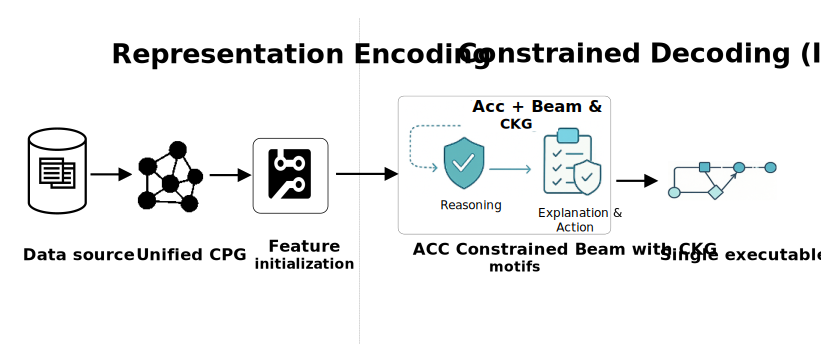
\includegraphics[width=\linewidth]{svg-inkscape/e2e.pdf}
	\caption{End-to-end pipeline for chain-centric vulnerability detection. Source repositories are parsed into a unified Code Property Graph (CPG), with GraphCodeBERT-initialized features providing input to a relation-aware encoder. At inference, ACC-constrained beam search guided by CKG motifs performs structured reasoning and outputs a single executable interprocedural chain, enabling interpretable vulnerability mechanisms.}
	\label{fig:intro-e2e-pipeline}
\end{figure}


% =========================================================
% 6) Methodological Overview
% =========================================================

\section{Methodological Overview}
\label{sec:intro-method}

This thesis develops a chain-centric, heterogeneous multigraph that integrates \emph{Abstract Syntax Trees} (AST), \emph{Control-Flow Graphs} (CFG), and \emph{Data-Flow Graphs} (DFG) within a \emph{Code Property Graph} (CPG). The graph is enriched with interprocedural semantics, namely a call graph, argument$\rightarrow$parameter and return$\rightarrow$caller bindings, call-site context, and coarse alias or points-to approximations, in order to capture realistic data and control transfers across functions and modules~\cite{yagemann2021automated}. Nodes and edges are initialized with structure-aware embeddings from \emph{GraphCodeBERT}, which encode lexical regularities together with data-flow cues learned from large code corpora~\cite{guo2021graphcodebert}. A graph attention encoder then aggregates neighborhood information across heterogeneous edges, and a \emph{flow-consistency} regularizer encourages attention to concentrate along CFG-reachable def--use chains and matched call or return links, while de-emphasizing edges that violate feasibility or typing constraints.

At inference, candidate chains are constructed by a constrained beam search. Adaptive Causal Contextualization (ACC) enforces execution feasibility (CFG/DFG reachability, well-nested call/return, alias consistency) while a lightweight Causal Knowledge Graph (CKG) contributes a score-only prior; formal definitions appear in §§\ref{sec:model-arch-gat}, \ref{sec:model-arch-ckg}, and \ref{sec:model-arch-acc}.

For training, the model employs a supervised vulnerability detection objective at the function or repository level, complemented by auxiliary regularizers that promote attention concentration on call and return edges implicated in positive samples and encourage sparsity in selected subgraphs to yield concise mechanisms. During inference, the encoder produces attention distributions and the system outputs both the prediction and its explanation (see §§\ref{sec:model-arch-acc}, \ref{sec:model-arch-extract-validate} for decoding details).

Evaluation combines standard performance metrics with two causality oriented measures. The \emph{Counterfactual Consistency Score} (CCS) tests prediction stability under principled interventions on chain elements for example, strengthening or inserting sanitization along a propagation edge or severing an argument$\rightarrow$parameter binding; edits to causal elements should reduce or flip the prediction, while changes to non-causal context should have minimal effect~\cite{Cao2024ICSE,Chu2024ISSTA}. The \emph{Causal Feature Attribution Measure} (CFAM) quantifies the proportion of attribution mass (attention or gradient-based importance) assigned to chain components sources, propagation links, and sinks versus off-chain context; with annotations it measures alignment, otherwise it tests internal consistency against frequency-matched but infeasible alternatives~\cite{Kuang2024KSEM,Rahman2024ICSE}. Together, CCS and CFAM evaluate the faithfulness and stability of reconstructed mechanisms beyond accuracy, complementing recent robustness- and explanation-oriented work~\cite{Cao2024ICSE,Cao2024ASE,Chu2024ISSTA,Chakraborty2020,Liu2020}.


\section{Dataset and Evaluation Preview}
\label{sec:intro-dataset}

The experimental evaluation utilizes the ReposVul dataset~\cite{wang2024reposvul}, a repository-level benchmark meticulously crafted to reduce patch entanglement and highlight explicit interprocedural structure.  ReposVul~\cite{wang2024reposvul} gives realistic examples of how to trace vulnerability mechanisms that affect more than one function or module by organizing vulnerable and fixed revisions at the repository level with detailed call relationships and multi-granular dependency annotations.  The experiments employ three standard splits, utilizing standardized preprocessing, stratified sampling, and controlled random seeds to ensure comparability and reproducibility. State-of-the-art graph neural network detectors and the causality aware COCA framework~\cite{Zhou2019,Cao2024ICSE} are two examples of baselines. Each one was carefully retrained on the same splits. 

The evaluation uses both traditional metrics and causal criteria. The Counterfactual Consistency Score (CCS) measures how stable a prediction is when the chain is changed on purpose, and the Causal Feature Attribution Measure (CFAM) measures how well attribution focuses on causal elements instead of incidental context.  In addition to standard detection metrics, I present chain-centric diagnostics (e.g., average chain length and interprocedural span) and incorporate concise case studies that illustrate hop-level justification for the constructed chains.  Robustness tests confirm invariance to benign code modifications, while qualitative case studies on reconstructed chains assess explanation fidelity and remediation efficacy.  This protocol allows for a thorough comparison of chain-centric causal analysis with robust learning-based baselines, evaluating both detection performance and the fidelity and implementability of vulnerability explanations.


\section{Significance and Impact}
This research alters the explanation of vulnerabilities from localized, retrospective feature highlights to a singular, executable interprocedural causal chain that traverses from the root cause to the exploitable sink. The research makes model predictions mechanistically interpretable by reconstructing how untrusted input enters the system, travels through control and data dependencies across functions, avoids or skips sanitization, and reaches a vulnerable operation. These chains provide developers with precise, traceable evidence explaining the presence of a vulnerability, along with clear guidance on its location and the steps required for remediation. This changes black-box detections into useful, verifiable information. This makes learning based vulnerability detection more reliable, open, and useful for real-world software security assurance.


% =========================================================
% 9) Thesis Outline
% =========================================================
\section{Thesis Outline}
Chapter~\ref{chap:method-architecture} (Method and Architecture) formalizes the unified CPG, feature initialization, relation-aware GAT, and the ACC decoding procedure with the CKG prior; Chapter~\ref{chap:evaluation} (Evaluation Protocol and Metrics) defines conventional, chain-centric, and causal metrics and describes calibration and intervention design; Chapter~\ref{chap:results} (Experimental Results and Analysis) reports quantitative and qualitative findings, ablations (ACC/CKG/beam), decoding profile, robustness, and comparisons to \emph{COCA}; Chapter~\ref{chap:conclusion} concludes with limitations and future directions. An artifact and dataset card appear in the appendix.





%========================================
% Chapter 2 — Literature review
%========================================






\chapter{Literature Review}

The increasing reliance on machine learning (ML) to analyze source code has fundamentally transformed the software security landscape. The growing need for more reliable and interpretable vulnerability detection has driven extensive exploration of deep learning (DL) approaches. Architectures notably Graph Neural Networks (GNNs) operating over program graphs-promise scalable vulnerability detection and localization by learning structure-aware representations directly from code, often surpassing the performance of traditional static and dynamic analysis. However, despite this success, important challenges persist: difficulties generalizing across projects and distributions, high sensitivity to spurious correlations, limited support for interprocedural reasoning, and explanations that are insufficiently faithful for developer remediation. This chapter synthesizes the trajectory from early DL-based vulnerability detection and model explanation to current causality-aware approaches. I give particular attention to the development of pre-trained structural encoders and the emerging need for datasets that better reflect interprocedural mechanisms, ultimately crystallizing the unresolved gaps that motivate the core contributions of this thesis.

\section{Theoretical Foundations and Background}


Here I consolidates the key theoretical concepts and technical background necessary for understanding the research presented in this thesis. It distinguishes software bugs from security vulnerabilities, reviews classical static and dynamic analysis, details canonical code representations that enable structurally informed reasoning, explains interprocedural semantics for modeling flows across function boundaries, and motivates the incorporation of causality and counterfactual reasoning into security analytics. Where appropriate, references to recent surveys and representative systems are provided to anchor definitions and scope \cite{Chakraborty2020,Liu2020}.

\subsection{Software Bugs and Vulnerabilities}
\label{sec:intro-bugs}

A \emph{bug} is a defect that causes a program to behave incorrectly or unexpectedly. Not all bugs threaten security. A \emph{vulnerability} is a defect that an adversary can exploit to violate confidentiality, integrity, or availability. Distinguishing benign errors from exploitable vulnerabilities requires understanding not only the defect itself but also the \emph{mechanism} by which it can lead to a successful attack.

This mechanism can be conceptualized as a chain of causation that begins at a \emph{root} condition (e.g., untrusted input, unchecked buffer length, use-after-free) and \emph{propagates} through assignments, parameter passing, return values, aliasing relations, and implicit flows induced by control dependence. The chain becomes exploitable when a tainted or unsafe state reaches a sensitive \emph{sink}, such as a buffer write, command/SQL execution, deserialization routine, or privileged operation. Executability depends on dominance and post-dominance of guards, exceptional paths, resource lifetimes, and other feasibility constraints. This thesis therefore treats vulnerabilities as \emph{root$\rightarrow$propagation$\rightarrow$sink} mechanisms to be reconstructed and validated end to end.

\subsection{Classical Program Analysis: Static and Dynamic}
\label{sec:intro-classical}

\textbf{Static analysis} reasons about program behavior without execution. It uses dataflow frameworks and abstract interpretation to approximate reachable states across all paths. Precision is governed by \emph{flow sensitivity} (does the analysis respect statement order?), \emph{context sensitivity} (does it distinguish call sites or call histories?), \emph{path sensitivity} (does it track path conditions across branches?), and \emph{heap/field sensitivity} (does it distinguish fields and heap objects). Interprocedural static analysis requires constructing and resolving call graphs (e.g., class hierarchy analysis, rapid type analysis, points-to based resolution) and often employs summary-based propagation or IFDS/IDE-style solvers for scalable, distributive problems. Alias and points-to analyses are critical because they determine whether references may refer to the same memory, thereby controlling precision of def--use reasoning. Static analysis scales and can identify candidate roots, propagators, and sinks early, but coarse abstractions or under-modeled sanitization may cause false positives.

\textbf{Dynamic analysis} executes the program (or symbolic abstractions) to observe concrete behaviors. Fuzzing mutates inputs to trigger failures; sanitizers instrument code to detect memory errors and undefined behavior at runtime; concolic/symbolic execution uses path constraints to steer toward hard-to-reach states. Dynamic analysis yields concrete \emph{witness traces} but faces input-space and path-explosion limits. In practice, static analysis can prioritize likely vulnerable chains, while targeted dynamic validation confirms executability. This complementarity is especially useful for interprocedural mechanisms that cross module boundaries and depend on calling contexts.

\subsection{Code Representations for Security Analysis}
\label{sec:intro-repr}

\textbf{Abstract Syntax Tree (AST):}
The AST encodes the hierarchical syntactic structure of source code, abstracting away punctuation to represent declarations, expressions, and statements. It supports parsing, symbol resolution, and scope management. By itself, the AST lacks explicit execution ordering and data provenance, limiting its utility for end-to-end vulnerability tracing.

\textbf{Control-Flow Graph (CFG):}
A CFG represents the flow of control between basic blocks, including exceptional control. Analyses derive dominance/post-dominance, loop structure, and reachability---all necessary for judging whether guarding conditions actually protect sinks. Interprocedural CFGs (ICFGs) connect call sites to callees and returns to callers, modeling control transfer across procedures and enabling reachability checks across functions.

\textbf{Data-Flow Graph (DFG):}
A DFG links definitions to uses (def--use chains), tracking value provenance across assignments, operations, parameter passing, and returns. Static Single Assignment (SSA) form simplifies reasoning by introducing $\phi$-nodes at merges. Interprocedurally, argument$\rightarrow$parameter and return$\rightarrow$caller bindings extend provenance across calls, while alias/points-to facts determine when references share storage.

\textbf{Program Dependence Graph (PDG):}
The PDG unifies data and control dependencies in a single graph, enabling slicing along both axes and reasoning about implicit flows. PDGs are commonly intra-procedural; explicit extensions are required to model interprocedural flows for whole-program reasoning.

\textbf{Code Property Graph (CPG):}
The CPG combines AST, CFG, and DFG into a heterogeneous, typed multigraph, supporting joint queries over syntax, execution order, and data dependencies \cite{yamaguchi2014cpg}. CPGs are well suited to vulnerability discovery because they admit taint-style queries that trace feasible paths from sources through transformations to sinks while retaining syntactic anchors for precise localization. For interprocedural analysis, the CPG is enriched with call-graph edges, argument$\rightarrow$parameter and return$\rightarrow$caller links, call-site context (e.g., dynamic dispatch), and coarse alias information, enabling faithful reconstruction of cross-boundary propagation. This thesis adopts an augmented CPG as the backbone for chain-centric mechanism tracing.

\textbf{Interprocedural Semantics:}
Executable vulnerability chains often cross function boundaries. To capture these flows, the representation integrates (i) a call graph, (ii) argument-to-parameter and return-to-caller relations, (iii) call-site contexts (e.g., receiver/dispatch in object-oriented code), and (iv) alias/points-to approximations. Together they support tracing explicit data flows and implicit control effects across modules in a way that aligns with feasible program execution.


\subsection{Learning over Program Graphs}
\label{subsec:learn-over-graphs}

Learning-based techniques complement classical analysis by operating directly on structured code graphs. In this view, programs are represented as heterogeneous graphs that merge AST, CFG, and DFG into a unified Code Property Graph (CPG), exposing typed nodes/edges (e.g., \texttt{CFG}, \texttt{DFG}, \texttt{CALL}, \texttt{ARG}\(\to\)\texttt{PARAM}, \texttt{RET}\(\to\)\texttt{CALLER}). Graph neural networks (GNNs) then propagate information along these relations to classify snapshots or localize vulnerable regions, with statement/line-level variants explicitly exploiting structure to sharpen localization \cite{Zhou2019,hin2022linevd,Chakraborty2020}. Relation-aware message passing and attention over edge types are particularly well-suited to interprocedural reasoning because they can weight control-, data-, and call/return links differently during aggregation.

Structure-aware pretraining further improves node/edge representations before graph reasoning. In particular, GraphCodeBERT injects data-flow awareness into transformer encoders and yields context-sensitive token embeddings that, when fused with structural channels, improve cross-project generalization \cite{guo2021graphcodebert,fu2022linevul}. In this thesis, such frozen language-model features provide a stable semantic channel, while the relation-aware GNN learns how evidence should travel across heterogeneous edges in the CPG.

Despite these advances, empirical studies consistently show degradation under benign refactorings and cross-repository transfer, revealing sensitivity to spurious, project-specific correlations \cite{Li2022Empirical,yang2022natural}. This motivates going beyond correlation-based detectors toward mechanisms that privilege executable flows. Recent lines of work introduce causal notions at different levels: contrastive/counterfactual training and inference (\emph{COCA}, \emph{CFExplainer}) \cite{Cao2024ICSE,Chu2024ISSTA}, causal adjustment and denoising to suppress non-causal context (\emph{Snopy}) \cite{Cao2024ASE}, and structural-causal formulations that prioritize features with genuine influence (\emph{VulCausal}, \emph{CausalVul}) \cite{Kuang2024KSEM,Rahman2024ICSE}. Broader explainability studies also highlight the gap between saliency-style rationales and truly causal explanations, calling for evaluations that test faithfulness and intervention stability \cite{Allix2024,li2023xai,Moschitti2024}.

These observations motivate the chain-centric stance taken here: use a unified, interprocedural program graph; learn relation-aware evidence propagation over it; and then \emph{constrain} decoding so that the returned explanation is a single, executable root\(\rightarrow\)propagation\(\rightarrow\)sink chain. Causal priors and structured decoding (detailed next) ensure that learned scores translate into mechanisms that remain valid under program semantics and robust under counterfactual edits.







\subsection{Causal-Guided Structured Decoding}
\label{sec:theory-ckg}

\paragraph{Causal Knowledge Graph(CKG):}
\label{para:rw-constrained-ckg}

The concept of a \emph{Causal Knowledge Graph (CKG)} has emerged in recent literature as a means of capturing the underlying mechanisms that explain \emph{why} specific structural or semantic relationships tend to follow one another, rather than merely documenting their co-occurrence~\cite{Kuang2024KSEM,Cao2024ICSE}. Within program analysis, such knowledge graphs enable models to represent and reason about directional causal dependencies between program relations. Unlike traditional graph structures, which primarily record entities and factual edges, a CKG encodes empirical patterns and causal tendencies, thereby providing a foundation for more interpretable, mechanism-aware reasoning~\cite{Rahman2024ICSE,Zheng2023CausalKG}.

In the context of vulnerability detection, this thesis leverages CKGs to model causal pathways underlying interprocedural vulnerability propagation~\cite{Kuang2024KSEM,Cao2024ICSE}. Nodes in the CKG correspond to relation types within heterogeneous program graphs, such as function calls, argument-to-parameter bindings, return-to-caller edges, or data-flow and control-flow links. Directed edges represent empirically observed transitions, indicating where one relation type tends to cause or enable another during the construction of vulnerability chains. Beyond simple one-step transitions, the CKG summarizes multi-step motifs—recurrent bi-grams and tri-grams—that characterize common propagation mechanisms in actual codebases. For instance, frequent motifs may describe a function call followed by argument propagation and then a return linkage, reflecting a typical cross-functional vulnerability transfer~\cite{Rahman2024ICSE,guo2021graphcodebert}.

The value of a CKG lies in its ability to guide learning systems away from brittle, correlation-driven associations. Purely data-driven detectors risk overfitting to locally prevalent regularities that lack mechanistic grounding, resulting in poor robustness under domain shift~\cite{Li2022Empirical}. A CKG estimated post hoc from training graphs acts as a lightweight structural prior, gently nudging chain assembly toward empirically plausible transition patterns without enforcing rigid rules or handcrafted heuristics~\cite{Kuang2024KSEM,Rahman2024ICSE}. This structure regularizes the inference process, reducing uncertainty and encouraging coherent, interpretable chain construction.

Construction of a CKG relies on analyzing relational evidence from large program datasets to derive statistically frequent transition patterns between relation types. These patterns are extended into higher-order motifs, creating a compact summary of causal sequence structures across interprocedural contexts. The resulting graph reflects both likely cause-effect transitions and interpretable motifs that can be visualized or audited by developers~\cite{Kuang2024KSEM,Zheng2023CausalKG}. Importantly, the CKG operates as an auxiliary, non-intrusive source of plausibility: learned evidence from the main detection model remains paramount, with the CKG acting as a gentle regularizer that rewards transitions reflecting historically robust causal structure.

Integration of a CKG into vulnerability detection aligns with ongoing research in explainable artificial intelligence and causal inference, which prioritize mechanistic interpretability over mere statistical association~\cite{Chakraborty2020,Moschitti2024}. Prior studies highlight the pitfalls of models lacking causal grounding, noting that visual explanations derived from attention or saliency scores often misrepresent the actual factors driving a prediction~\cite{Chakraborty2020,Cao2024ASE}. By explicitly encoding directional causal patterns among program relations, the CKG supports stability and transparency in chain reconstruction. Each causal link can be contextualized within a known relational motif, making the resulting causal pathway auditable and actionable for developers~\cite{Kuang2024KSEM,Chu2024ISSTA}.

Overall, while traditional knowledge graphs serve mainly as record-keepers for observed facts, a CKG distinguishes itself by focusing on mechanistic tendencies and supporting reasoning under hypothetical interventions, such as what happens when a relation is inserted, altered, or removed. This ability to model executable vulnerability chains with explicit causal grounding positions CKGs as essential tools in mechanistic vulnerability analysis, where understanding the propagation mechanism is as important as detecting the flaw itself~\cite{Kuang2024KSEM,Cao2024ICSE,Rahman2024ICSE}.

\paragraph{Constrained Decoding and Beam Search for Structured Reasoning:}
\label{para:rw-constrained-beam}

Beam search has become a widely adopted heuristic for navigating complex structured search spaces, enabling the efficient identification of high-quality candidate solutions by maintaining a finite set of top-scoring partial hypotheses at each expansion step~\cite{RussellNorvig2020AI}. This approach balances exploration with computational tractability, making it particularly useful in combinatorial prediction tasks. In the context of structured reasoning and program analysis, however, conventional beam search and naive methods such as best-first or depth-first search often struggle with the feasibility constraints imposed by programming language semantics and logical requirements. These unconstrained strategies can produce locally optimal but globally invalid paths, resulting in interpretations or program traces that do not respect the logic of the system.

The concept of \emph{constrained decoding}, also known as guided beam search, addresses this limitation by enforcing domain-specific validity criteria during the search process~\cite{Martins2022StructuredDecoding}. In constrained beam search, candidate expansions are dynamically filtered or weighted based on both hard structural constraints (e.g., grammar rules, type safety, execution order) and soft statistical preferences drawn from prior knowledge or data. For program graph reasoning, these constraints typically include control- and data-flow consistency, legality of interprocedural transitions (such as proper function call/return matching), avoidance of cycles or infinite recursion, and aliasing concerns. Incorporating these checks ensures the resulting reasoning chains or traces correspond to paths that are executable and semantically valid, preserving logical coherence across function and module boundaries~\cite{Chu2024ISSTA}.

Practical applications of constrained beam search span diverse structured prediction problems such as syntactic parsing~\cite{Freitag2017Parsing}, symbolic program execution~\cite{Li2022Empirical}, knowledge graph inference, and code generation. Earlier methods often relied on hand-crafted heuristics or deterministic rules for pruning search paths, while others introduced scoring functions based on local learned features. However, exclusive dependence on heuristics can fail to adapt across domains, and purely data-driven scoring may lack generalizability and fall prey to spurious correlations. Addressing these shortcomings, recent research integrates statistical priors mined from empirical data, such as edge-gram or motif frequencies directly into the decoding process. These data-driven priors help guide the search toward patterns historically associated with correctness, blending empirical knowledge with strict legality filters~\cite{Kuang2024KSEM,Rahman2024ICSE}.

Compared to more global but computationally intensive optimization methods like Integer Linear Programming (ILP) or Satisfiability Modulo Theory (SMT) solving, constrained beam search achieves a practical and interpretable compromise~\cite{mandal2020solving}. It enables efficient exploration of numerous plausible causal chains, generating a ranked collection of candidate explanations suitable for developer inspection and verification. The synergy between legal constraint enforcement and empirical causal priors produces a decoding process that is both mechanism-aware and computationally tractable, thereby supporting the broader goal of generating structured, executable explanations that faithfully represent how vulnerabilities propagate in complex software systems.




\section{Related Works}

\subsection{Static Analysis: Foundations and DL Integration}

Static analysis examines software artifacts without executing them, reasoning exhaustively about possible program behaviors through frameworks like lattice-based dataflow analysis and abstract interpretation \cite{yamaguchi2014cpg, Chakraborty2020}. Its precision depends on sensitivities to control flow, call context, execution paths, and heap or field representations. Interprocedural static analysis demands accurate call graph construction, supported by methods such as Class Hierarchy Analysis, Rapid Type Analysis, and points-to analyses to resolve aliasing \cite{Xia2023, Liu2020}.

These analyses utilize canonical program representations: Abstract Syntax Trees (ASTs) encode syntactic structure; Control-Flow Graphs (CFGs) model executable order and branching; Data-Flow Graphs (DFGs) trace variable value definitions and uses; and Program Dependence Graphs (PDGs) unify data and control dependencies for program slicing. The Code Property Graph (CPG) integrates AST, CFG, and DFG into a heterogeneous multigraph that supports global queries essential for interprocedural taint tracking from sources to sinks \cite{yamaguchi2014cpg}.

Despite early identification benefits, classical static analysis suffers from false positives due to over-approximation in modeling sanitizers, aliasing, and dynamic dispatch \cite{Ruiz2023, Marchetto2024}. Automated static analyzers such as Flawfinder, RATS, CPPCheck, SpotBugs, and PMD show variability in detection accuracy and false positive rates across languages like C++ and Java \cite{Kaur2020comparative}. These limitations motivate the development of DL-augmented static analysis tools. For example, IRIS incorporates large language models (LLMs) with static analysis to infer taint specifications and improve vulnerability detection coverage and false discovery rates, surpassing traditional tools like CodeQL \cite{Li2024IRIS}.

Further, hybrid approaches blend static analysis with ML classifiers to filter and prioritize warnings, addressing false positives and improving scalability \cite{hu2023hybrid}. Static analysis remains foundational, providing structured input to DL models, yet its limitations in handling complex, evolving, and domain-specific codebases remain a persistent challenge \cite{Xia2023, Chakraborty2020}.

\subsection{Dynamic Analysis: Execution Evidence and DL Integration}
Dynamic analysis observes real or symbolic execution of programs with concrete inputs to detect vulnerabilities manifesting during runtime \cite{yagemann2021arcus, yagemann2021automated}. Techniques include fuzzing, which automates input mutation to explore program paths; sanitizers, which instrument binaries or source to catch memory errors; and symbolic or concolic execution, which employs solvers to systematically explore feasible paths leading to fault states.

Dynamic methods provide high precision witness traces, essential for actionable debugging, but suffer from path explosion and limited environmental coverage, particularly in large interprocedural contexts \cite{yagemann2021arcus}. This gap has incentivized hybrid strategies integrating machine learning to guide input generation or prioritize suspicious execution traces, enhancing coverage efficiency \cite{xu2023mlforfuzzing}.

Recent work employs reinforcement learning and deep models to optimize fuzzing or dynamic analysis workflows, combining symbolic constraints and learned heuristics to uncover hard-to-detect vulnerabilities \cite{tufano2022adaptive}. These advances promise better balancing precision and exploration in complex, modern software systems.

Dynamic analysis's concreteness complements static analysis’s scalability, and their integration with machine learning techniques is an active research frontier poised to improve vulnerability detection coverage, efficiency, and interpretability.



\subsection{Deep Learning Based Techniques}

Deep learning is transforming many areas of computer science and has been applied in research projects. In particular, graph neural networks (GNNs) \cite{hin2022linevd}, deep learning models have rapidly shown their promise in vulnerability detection, achieving amazing precision in identifying susceptible code patterns \cite{chakraborty2021deep, Liu2020, Yaqin2020}. GNNs offer a natural approach for capturing complex software dependencies by modeling code as graphs, using nodes for elements (e.g., variables, functions) and edges for relationships (e.g., data flow, control flow). Hin et al. \cite{hin2022linevd}, for instance, showed how well GNNs identified vulnerabilities at the statement level. With the capacity to learn from the structure and semantic information of code, the models were able to spot vulnerabilities suggestive of buffer overflows or injection issues. Although many of these early deep learning models functioned as "black boxes," impairing the knowledge of their decision-making processes \cite{li2023vulanalyzer, mosolygo2021towards}, even with their precision. Especially in the context of software security, the ability to understand the reason \emph{why} a model finds a piece of code as vulnerable is crucial for developers to implement fixes \cite{USGov2023}. This lack of transparency is a major concern. Furthermore, impeding the acceptance of these approaches in practical software development processes is their difficulty in explaining model predictions. The US Government's executive order \cite{USGov2023} on the safe, secure, and trustworthy development and use of artificial intelligence emphasizes how much artificial intelligence (AI) is becoming relied upon in important systems, where erroneous or untrustworthy predictions can have severe consequences.

Zhou et al. \cite{Zhou2019} presented a comprehensive comparative analysis of factors influencing the performance of deep learning (DL)-based vulnerability detection systems. Recognizing the complexity of software vulnerabilities, the authors sought to systematically evaluate how different design choices affect detection efficacy. To this end, they constructed two distinct datasets, capturing both data reliance and control dependencies extracted from programs, encompassing a diverse set of 126 different vulnerability types. Their methodology involved assessing the quantitative impact of several key elements on vulnerability identification performance. This included employing techniques for handling unbalanced data, incorporating control dependence information within code representations, and experimenting with various neural network architectures. To facilitate their analysis, Zhou et al. built a DL-based vulnerability detection system leveraging Joern, an expanded open-source code parser. The primary contribution of this work lies in its systematic assessment of the quantitative influence of these elements on vulnerability detection efficacy. The study's results offer valuable insights into the design and development of effective deep learning-based vulnerability detection systems. However, it's important to note that this research did not specifically address causal deep learning (CDL) or explicitly incorporate causal reasoning principles. The authors themselves highlighted the need to accommodate a wider range of vulnerability types, enhance the representation of code features, and overcome the limitations of relying solely on control and data dependencies. 

Li et al. \cite{Li2022Empirical} performed empirical research on deep learning (DL) models for vulnerability detection. On Devign and MSR data, they polled and replicated nine state-of-the-art (SOTA) models. They looked at and examined model capabilities (agreement, variability, performance on several vulnerability categories, and difficulties in addressing particular code aspects). They investigated how model performance responded to project mix and training data size. They identified significant code aspects applied for prediction using model explanation tools. The main contribution of the writers was a thorough investigation of models of deep learning vulnerability detection. For assessing and contrasting several deep learning models for vulnerability identification, this research offers a useful standard. Still, this study paid little attention to causative factors. The writers urged more investigation on code patterns, possible inclusion of causal detection for better generalization, and addressing of the shortcomings of present model interpretation techniques.

Zou et al. \cite{Zou2020} tackled this problem with domain adaptation methods and deep learning. To reduce distribution discrepancies between domains, their CD-VulD system learnt cross-domain representations. Learning token embeddings for generalization across tokens, the CD-VulD system transforms software program representations into token sequences. Abstract high-level representations based on those sequences are built using a deep feature model. Minimizing the distribution divergence between the source and destination domains helps to train cross-domain representations using the metric transfer learning framework (MTLF). The key contribution of the authors was a CD-VulD system learning cross-domain representations of source code via domain adaptation and deep learning. Practical vulnerability identification depends on generalizing across several fields, as models trained on one dataset might not work on another. This research did not, however, use causal reasoning; the authors observed constraints in evaluation scope and dependency on particular architectures.

\subsection{Causal Reasoning and Causal Deep Learning Techniques}

Conventional deep learning techniques have shortcomings, including their capacity to detect erroneous correlations and changes in dataset distribution. Stronger and broader methods have emerged from this. VulCausal, developed by Kuang et al. \cite{Kuang2024KSEM}, solves what caused what in neural network models. Finding and eliminating bogus links between API functions, user-defined names, and code structure is VulCausal's primary objective. The authors provide a structural cause model to demonstrate how discovering vulnerabilities is affected by user-defined names, API library IDs, and code structure. The study employs covert adjustment in the reasoning stage to eliminate erroneous correlations and minimize the impact of confounders. By modeling and lowering spurious correlations, VulCausal aims to make vulnerability identification more accurate and consistent than conventional deep learning approaches. This is a crucial first step toward exposing vulnerabilities. The writers mostly included a causal perspective to eliminate misleading correlations and provide more accurate and reliable vulnerability detection. When causal inference techniques were developed, they connected with a whole new level and helped us to better understand the factors causing vulnerability in individuals. One significant fresh concept is the application of backdoor correction and causal reasoning approaches. The approach wasn't flawless, the writers noted, though, as it lacked scalability to extremely big codebases, it wasn't ubiquitous across many computer languages, and it couldn't show direct causality (beyond performance benefits). This indicates that in these fields additional research is required. One should also consider the extent of labour causal inference techniques demand and the requirement of well crafted models. Zelikman et al. \cite{Zelikman2023} on self-taught optimizers also indicate that individuals are still striving to create machine learning models that are more efficient and helpful.

Le et al. \cite{Le2024MBU} investigated how well existing deep learning-based detectors could handle vulnerabilities spanning several base units of code (MBUs). Their empirical evaluation of current deep learning-based detectors revealed a clear deficiency in tackling MBU vulnerabilities, usually overstretching accuracy by focusing on individual base units (IBUs). Although it did not specifically include causal reasoning in the detection technique, this research underlined the need of investigating the features and distribution of MBU vulnerabilities as well as the limits of current datasets. Together with a detailed analysis of their incidence and detection accuracy in modern deep learning (DL)-based detectors, the authors gave a description and categorization of MBU vulnerabilities. The key contribution of the authors was the proposal of a framework for the correct integration of MBU vulnerabilities in DL-based detection. The study emphasizes the significance of evaluating the spectrum of vulnerabilities and of studying detection methods. The problem of MBU vulnerabilities is particularly relevant in modern software development, as code usually involves numerous files and modules. Furthermore, improving the understanding of vulnerability types and their frequency is the research by Nong et al. \cite{Nong2023ICSE} on authentic vulnerability generation through pattern mining and deep learning and the study by Woo et al. \cite{Woo2023USENIX} on identifying 1-day vulnerabilities in reused open-source software components.

Cao et al. \cite{Cao2024ASE} proposed Snopy, a deep learning (DL)-based technique bridging sample denoising with causal graph learning to enhance vulnerability identification. Snopy expressly included causal reasoning utilizing a Causality-Aware Graph Attention Network (CA-GAT), a Feature Caching Scheme (FCS), and a Causality-Aware Graph Attention Network (CA-GAT) identifying bogus features. Though areas for future research remain, including generalizability to other programming languages and vulnerability types \cite{Woo2023USENIX} and more sophisticated ways for mitigating spurious correlations in code, this approach represented a major step toward causal vulnerability detection. Initially, deleting vulnerability-irrelevant code elements and constructs using change-based sample denoising and then developing a Causality-Aware Graph Attention Network (CA-GAT) utilizing Feature Caching Scheme (FCS), Snopy learns causal vulnerability traits. The main contribution of the authors was a change-based method guided by vulnerability-fixing commits (VFCs) automatically removing vulnerability-irrelevant code components. A unique addition is made by the combination of sample denoising with causal graph learning; the usage of VFCs offers a moral approach to finding and eliminating pointless code components. Building strong and dependable vulnerability detection systems depends on one being able to differentiate between causal and spurious aspects.

Ganz et al. \cite{Ganz2024} focused on addressing data quality, model interpretability, robustness, and contextual sensitivity, thereby enhancing the usefulness of machine learning (ML)-driven vulnerability identification. This research particularly applied causal learning approaches to reduce confusing effects and improve detection robustness. They developed datasets by using a novel neural code augmentation technique. They assessed explanation tactics using a novel approach based on dynamic program analysis. They assessed models on their acquired biases using a novel assessment system based on causal learning. The main contribution of the authors was to provide strategies raising the relevance of learning-based vulnerability detection in practical environments. The study underlines the need to attend to pragmatic issues such as data quality and model interpretability. Relevant to the problems of model interpretability and explainability is the research by Suneja et al. \cite{suneja2021probing} on evaluating model signal-awareness by means of prediction-preserving input minimization, together with the study by Yu et al. \cite{yu2023counterfactual}.

Growing interest in causal deep learning (CDL) results from the limits of current approaches, especially in terms of generalization and the capacity to find the underlying causes of vulnerabilities. By means of CausalVul, Rahman et al. \cite{Rahman2024ICSE} directly addressed the lack of resilience and generalization to out-of-distribution (OD) data in deep learning (DL)-based vulnerability detection. Explicitly leveraging do-calculus and the backdoor criterion, this two-stage approach aimed at identifying and eliminating false features using causal learning algorithms. This paper clearly shows a clear improvement in causal deep learning (CDL) for vulnerability detection, therefore highlighting the possibilities of causal inference to increase model generalization. The correlations between code features and the vulnerability label were shown by the authors using a causal graph. They then trained models that were less dependent on spurious features and more focused on causal features by the use of do-calculus and the backdoor criterion. The main contribution of the authors was to explicitly address false correlations, thereby introducing a fresh method to increase the generalization and resilience of deep learning (DL)-based vulnerability detection. Two important developments are the application of the backdoor criterion and do-calculus. Real-world applications depend on generalizing OOD data since the spread of vulnerabilities may evolve with time.

Chu et al. \cite{Chu2024ISSTA} addressed the lack of explainability in Graph Neural Networks (GNNs) for vulnerability identification. Using counterfactual reasoning, a type of causal inference, CFExplainer aimed to identify minimal changes to the input code graph that would influence the GNN prediction. This improved explainability by focusing on behaviours that alter the outcome and so provides a "what-if" analytical capability. The approach finds a minimum disruption in the code graph by inverting the prediction of the GNN. This provides developers with useful knowledge and guides them on the necessary changes to eliminate a vulnerability. The authors mostly contributed by developing a counterfactual explanation method for GNN-based vulnerability discovery. Counterfactual thinking helps developers find a more reasonable and workable argument. A better basis for understanding the application of counterfactual reasoning in explainable artificial intelligence is provided by the work of Lucic et al. \cite{lucic2022cf}.

Islam et al. \cite{Islam2024} presented T5-GCN for vulnerability categorization, localization, and root cause identification. Although the "root cause" was sought for, this research did not specifically use causal deep learning (CDL), causal inference, or causal reasoning methods. Conversely, the explainability part of T5-GCN aims to identify the "root cause" of vulnerabilities, therefore indirectly guiding knowledge of the elements generating the vulnerability. The approach uses DeepLift-SHAP attribution values to determine the relevance of tokens in the code, therefore identifying the basic cause. Along with their classification, location, and a brief static description, the writers mostly contributed a method employing explainable methodologies to identify the root cause of a vulnerability. One original method is to combine GCNs and LLMs. Large language models (LLMs) for code analysis are a fast-expanding field of research; the research of Zelikman et al. Furthermore underlined in \cite{Zelikman2023} on self-taught optimizers, the potential of LLMs in this field is relevant for the application of LLMs in code analysis, and vulnerability detection is the effort of Pearce et al. \cite{pearce2025asleep} to assess the code contributions' security of GitHub Copilot.

Cao et al. \cite{Cao2024ICSE} presented Coca, a framework to enhance the causality and robustness of Graph Neural Networks (GNNs)-based vulnerability detection systems. Coca used dual-view causal inference, that is, factual and counterfactual reasoning, to pinpoint code statements most likely to be decisive for vulnerability discovery. This method showed a sophisticated use of causal ideas to solve constraints in robustness and explainability observed in past GNN-based detectors. It also underlined the difficulties in juggling concision with effectiveness in explanations. Coca trains GNNs less prone to false correlations and more focused on real vulnerability traits by means of combinatorial contrastive learning. The Explainer component generates succinct and powerful explanations using dual-view causal inference. Using supervised constrastive learning, the system is taught to identify the bug in all versions and distinguish between buggy and non-buggy code. It discovers a flaw and then employs factual and counterfactual thinking. This is a framework enhancing the causality and dependability of GNN-based vulnerability detection systems. 

\subsection{Explainability and Interpretability Techniques}

In the first attempt to tackle the explainability issue, scientists aimed to create techniques that would reveal the inner workings of deep learning models, hence enabling more reasonable and reliable predictions. Proposed by Le et al. \cite{li2023vulanalyzer}, GAVulExplainer was one of the first attempts to handle this using a model-agnostic approach, that is, one can apply GAVulExplainer to several deep learning models and genetic algorithms to help find important subgraphs causing vulnerabilities. The basic concept is to build a subgraph emphasizing the important elements causing the vulnerability, therefore offering a more understandable justification for the predictions of the model. While avoiding local optima, the genetic algorithms effectively seek accurate substructure information. This method employs a fidelity metric to assess the quality of produced explanations and lets users regulate the size of the explanation subgraph. GAVulExplainer marks a significant progress in enhancing the interpretability of GNN-based vulnerability detection, but it still lacks explicit modeling of the fundamental \emph{causal} links between code characteristics and vulnerabilities. Finding contributing subgraphs still takes front stage without exploring causal deep learning (CDL) methods. Furthermore, its assessment depends on fidelity criteria, which might not completely reflect the pragmatic value of the explanations for developers in real-world debugging situations, especially given the complexity of software systems and the several ways vulnerabilities might show themselves. This study addressed the demand for explainable prediction since they realized that successful remedial action and developer confidence depend on knowing the "why" behind the prediction of a model.

Li et al. \cite{li2023vulanalyzer} presented that Vulanalyzer is another significant initiative aimed at improving explainability. Specifically developed for binary detection, a rather difficult subject given the low-level features of binary code, this deep learning model, Vulanalyzer, accurately preserves instruction semantics and structural linkages by using sequential and topological learning to mimic program execution through recurrent units and graph convolution, especially in assembly code \cite{taviss2024asm2seq}. Mostly distinguished by its multi-head attention system, which stresses pertinent commands and fundamental blocks, Vulanalyzer underlines fundamental directions and basic blocks. This encourages developers to concentrate on the code components the model considers most indicative of a vulnerability, therefore producing interpretable results. Although it clarifies things, Vulanalyzer, like GAVulExplainer, does not especially mix causal reasoning, causal inference, or causal deep learning (CDL). Emphasizing the need of greater study on causal approaches that can identify the why behind vulnerability projections, the emphasis stayed on simplifying difficult interactions and improving interpretability by means of attention processes. The writers mostly concentrated on the lack of explainability and the challenges to elucidate intricate links in binary code. With topological and sequential learning combined, the approach captures structural relationships as well as instructional meanings, so requiring minimal topic knowledge. Still, even if attention processes help to define the what of the model's judgments, they do not naturally define the \emph{why} - the fundamental causal factors generating the sensitivity. Most importantly, the method can be applied over multiple architectures and code obfuscation methods. The research on the development of explainable functional summaries of assembly code performed by Taviss et al. \cite{taviss2024asm2seq} emphasizes understanding code semantics in vulnerability analysis.

Moschitti et al. \cite{Moschitti2024} presented an XAI-based system for assessing computer code in a graph environment. This system evaluates the significance of syntactic structures for Common Weakness Enumeration (CWE) classification \cite{li2023xai}, therefore connecting learnt code feature representations to subtle semantics recognized by security professionals. The system generates ranks of syntactic constructive contribution levels in Abstract Syntactic Trees (AST) among CWE types for Java and C++ datasets. A novel feature-masking method, varying the neighbourhood of code tokens and syntactic constructions, is applied for the graph environment. The change in the code token neighbourhood is transformed into the CWE-type similarity score by means of information retrieval approaches. The authors showed how nuanced semantics understood by security professionals might be connected to the learnt code feature representations by CWE similarity generated from XAI explanations. This approach did not, however, particularly target causal reasoning or causal deep learning (CDL). The authors admitted that present XAI systems have several limits, namely, their incapacity to generalize to undiscovered vulnerability patterns and transcend the scope of input data. The constraints covered are those of interpretability of acquired features and transferability of learned patterns to different datasets. Although graph-based representations and ASTs are widely used in vulnerability identification, their efficacy may vary depending on the programming language and the particular vulnerabilities under attack. The research of Allamanis et al. \cite{Xia2023} on machine learning for massive code and naturalness offers a larger background for appreciating the difficulties of expressing and evaluating code.

Hajipour et al. \cite{Hajipour2023} developed a framework for vulnerability threat prediction. This method generated a semantic representation and computed an explainable threat score by prioritizing research activities using topic modeling of vulnerability descriptions (from sources like the National Vulnerability Database). Furthermore, included was a fresh trend score based on internet infosec conversations to pinpoint popular vulnerabilities. These results were aggregated on a visual dashboard to give investigative work top priority. The main contribution of the authors was the computation of a new trend score and an explainable threat score based on the topic model. This framework offers a semantic representation of vulnerabilities constructed using topic modeling of vulnerability descriptions. The framework offers a semantic representation of vulnerabilities constructed using topic modeling of vulnerability descriptions. Although helpful for prioritizing, it did not investigate the fundamental \emph{causal} elements affecting vulnerability exploitability, like particular code patterns or interactions increasing the probability of the exploitation of a vulnerability. Understanding which vulnerabilities are most likely to be exploited aids in prioritizing risk management efforts. Existing frameworks often rely on online discussions and external vulnerability descriptions, which may introduce biases and limit timeliness and completeness.

Allix et al. \cite{Allix2024} investigated the use of deep learning and explainability methods (most especially SHAP) toward this aim. Their results showed that explainability techniques might occasionally present distracting information, therefore harming rather than supporting engineers; code characteristics employed by DL models were often only partially connected to the underlying causes of vulnerabilities. This emphasized the need for more accurate localization and the incorporation of causal reasoning to uncover the true underlying causes. This allows for a deeper understanding that goes beyond mere correlations. The main contribution of the authors was to assess how well explainability and deep learning (DL) approaches could localize source code assertions concerning vulnerabilities. Using two deep learning (DL) techniques, VulDeePecker and JavaBert, the authors localized source code phrases pertaining to vulnerabilities using SHAP, a model-agnostic explainability method. The paper emphasizes that current explainability methods do not provide developers with practical insights effectively. Important determinants of the results of the study are the choice of deep learning models (VulDeePecker and JavaBert) and the respective application of SHAP. Practical implementations depend critically on more programming language-oriented encoding approaches recommended by Allix et al. \cite{Allix2024} and the evolution of more advanced techniques for vulnerability localization.


\section{Research Gaps}

Despite substantial empirical success achieved by deep learning (DL) approaches in software vulnerability detection, several fundamental limitations persist that compromise the reliability, generalization, and actionable utility of these systems in industrial settings. These deficiencies collectively define the necessity for the proposed research framework.

\paragraph{The Causal Deficiency and Generalization Gap:}
The first major challenge stems from the inherent reliance on statistical correlations over genuine causal mechanisms in program analysis. Current detectors frequently learn surface-level regularities or spurious correlations that co-occur with vulnerabilities in training data. This methodological bias compromises model robustness, manifesting as fragility under benign code transformations and significant performance degradation during cross-project domain shift. This brittleness suggests that existing normalization or domain-adaptation strategies only partially mitigate the underlying causal deficiency, leading to unstable predictions and poor transferability in dynamic, evolving code repositories. Consequently, many models fail to capture the true generative flaw mechanism.

\paragraph{The Interprocedural Reasoning Gap:}
The second critical deficiency is the limited capability for interprocedural reasoning and mechanism reconstruction. The majority of current learning frameworks are constrained to analyzing function-level slices or local subgraphs. This constraint prevents them from effectively tracing the end-to-end vulnerability lifecycle: the root cause $\rightarrow$ propagation path $\rightarrow$ exploitable sink. Without a mechanism-aware representation that explicitly models data and control dependencies across function boundaries, detectors default to highlighting local saliency, failing to reconstruct the comprehensive, executable narrative required by developers for complete, verifiable remediation.

\paragraph{The Causal Evaluation Gap:}
A third limitation concerns evaluation. Standard metrics such as Accuracy, Precision, Recall, F1, and mAP quantify label agreement but do not assess whether a model’s attributions are causally faithful or stable under principled counterfactual edits. In the absence of standardized \emph{causal} metrics, it remains difficult to determine whether a detector has learned the generative mechanism of a vulnerability or merely a pattern correlated with it.

\bigskip\noindent
To address these gaps, a novel framework is required, one that integrates causal
reasoning, contextualization, and attention-driven graph-based learning. Such a system must be capable of identifying spurious correlations and performing a counterfactual analysis. It should construct contextual causal chains that trace how vulnerabilities propagate across components, monitor causal evaluation metrics to ensure transparency, and leverage graph-based neural networks to effectively capture interprocedural dependencies. In addition, it should implement context-sensitive attention mechanisms to prioritize the most security-relevant code segments.


\section{Research Challenges and Rationale}
\label{sec:litreview-challenges}

The field of automated vulnerability analysis has progressed considerably over the past few years, yet several fundamental challenges continue to limit both reliability and interpretability. A closer reading of the literature reveals that many reported improvements in predictive accuracy obscure issues that have practical consequences for real-world deployment. Publicly available corpora often contain near-duplicate samples, mislabeled or weakly supervised instances, and severe class imbalance, all of which inflate apparent performance gains and make reproducibility difficult to achieve~\cite{Li2022Empirical,Chakraborty2020}. Moreover, a substantial portion of existing datasets are trimmed to function-level snippets that conceal the cross-function control and data flows from which actual exploits emerge. While newer datasets have made progress in improving curation and granularity, comprehensive resources remain rare. The \emph{ReposVul} dataset represents a notable advancement by preserving repository-level context with multi-granular dependencies and explicit call relations~\cite{wang2024reposvul}; however, the research community still lacks standardized multi-factor benchmarks capable of jointly evaluating accuracy, robustness to benign code transformations, interprocedural coverage, and explanation quality across root, propagation, and sink components. The absence of such benchmarks makes it difficult to measure generalization beyond narrow or synthetic settings, thereby slowing the transition of academic progress into practice.

Representation remains a pivotal element in achieving reliable and interpretable vulnerability detection. Sequence-based models, including transformer architectures, perform competitively in benchmark settings but struggle to capture control and data dependencies that underlie real exploitability~\cite{fu2022linevul,Chakraborty2020}. In contrast, graph-based representations such as Abstract Syntax Trees (AST) for syntactic structure, Control-Flow Graphs (CFG) for execution order, Data-Flow Graphs (DFG) for variable influence, Program Dependence Graphs (PDG) for joint control-data dependence, and Code Property Graphs (CPG) for unified representations~\cite{Zhou2019}, have shown promise in encoding the structural context critical to vulnerability comprehension. Yet, empirical performance remains highly sensitive to how interprocedural semantics are represented specifically, the inclusion of call edges, argument$\rightarrow$parameter and return$\rightarrow$caller bindings, and approximations for aliasing or points-to relationships. Structure-aware pretraining frameworks such as \emph{GraphCodeBERT} have improved downstream generalization by incorporating data-flow signals into token-level embeddings~\cite{guo2021graphcodebert,Li2022Empirical}. However, the extent of this improvement depends heavily on granularity, dataset diversity, and the quality of interprocedural signal integration.

Beyond static representation, the process of assembling long, executable vulnerability paths from root cause to sink presents an additional challenge that is both combinatorial and semantic. Naive best-first or depth-first search strategies tend to drift into locally plausible but globally inconsistent chains, while global optimization strategies such as Integer Linear Programming (ILP) or Satisfiability Modulo Theory (SMT) are computationally intractable at practical scales. This exposes a structural gap in current systems, where many either perform unconstrained search, leading to instability and irreproducibility, or depend on handcrafted heuristics that fail to capture the genuine progression of interprocedural flaw propagation. The research presented here addresses this issue by employing a \emph{constrained beam search} procedure enhanced with an \emph{Adaptive Causal Contextualization (ACC)} layer that enforces structural constraints including control- and data-flow reachability, interprocedural legality, and cycle avoidance. Additionally, a compact \emph{Causal Knowledge Graph (CKG)} is mined from training data to serve as a small but informative prior over relation $n$-grams. This CKG encodes directional motifs derived from empirical code patterns, gently biasing the decoding process toward realistic causal transitions without overriding correctness validations performed by ACC. The combination of structured constraints and empirical causal priors reduces search entropy and improves the stability and coherency of long interprocedural traces.

Another enduring barrier to adoption is model brittleness under realistic development environments. A wide range of architectures spanning LSTMs, graph neural networks (GNNs), and transformers have demonstrated significant degradation when transferred across projects, programming styles, or naming conventions~\cite{Li2022Empirical}. Even minor, semantics preserving edits can cause large fluctuations in predictions. While model adaptation strategies mitigate these effects to a degree, most existing pipelines remain correlation driven and fail to develop explicit awareness of causal mechanisms~\cite{Zou2020}. Furthermore, a persistent simplifying assumption in the literature is that vulnerabilities exist within isolated functions, leading to overly optimistic performance estimates that overlook cross-component propagation and realistic exploit surfaces~\cite{Le2024MBU}. Post-hoc explanation techniques, including attention visualization and perturbation analysis, have been widely applied, but these often highlight spurious or overly localized features that do not align with the actionable causes developers must address~\cite{Allix2024,Moschitti2024}.

Recent research trends have increasingly turned toward causality-aware learning, encompassing counterfactual training formulations, dual factual–counterfactual evaluation strategies, and graph-based editing techniques designed to test causal stability~\cite{Cao2024ICSE,Chu2024ISSTA,Rahman2024ICSE,Kuang2024KSEM,Cao2024ASE}. While these methods offer improvements in robustness and interpretability, the field still lacks consensus metrics for quantifying causal fidelity specifically, the stability of model predictions under targeted interventions and the alignment of internal attributions with ground-truth causal elements. These limitations define the core motivation for this research.

The work undertaken in this thesis specifically addresses these gaps by focusing on interprocedural vulnerabilities that propagate across functions, files, and modules. Programs are encoded as enriched Code Property Graphs with explicit cross-boundary semantics, enabling faithful modeling of causal dependencies. Using \emph{constrained beam search} guided by \emph{Adaptive Causal Contextualization (ACC)}, and assisted by a lightweight \emph{Causal Knowledge Graph (CKG)} prior derived from frequent relational motifs, the proposed framework explicitly constructs a single, executable root$\rightarrow\cdots\rightarrow$sink causal chain for each detected vulnerability. This approach ensures both structural legality and semantic plausibility throughout the reasoning process. To determine whether the model captures underlying mechanisms rather than dataset-specific correlations, conventional detection metrics are complemented by causal criteria that evaluate predictive stability under intervention (counterfactual consistency) and structural attribution alignment. Collectively, these components yield a chain-centric, interprocedural, and causally principled methodology aimed at producing transparent, auditable explanations that developers can meaningfully interpret, validate, and act upon.



%========================================
% Chapter 3 — Methodology
%========================================
\chapter{Methodology}
\label{chap:method-architecture}

This chapter presents the complete learning pipeline developed for this thesis, designed to achieve two complementary objectives: accurate vulnerability detection and faithful reconstruction of executable interprocedural causal chains. The overarching goal is not merely to identify code fragments that are susceptible to exploitation but to connect each vulnerability’s root cause to its propagation and eventual sink through semantically meaningful, executable paths. This approach directly addresses the interpretability and robustness limitations of existing deep learning models, which often identify vulnerable statements in isolation without reconstructing their broader causal mechanisms.

The proposed methodology builds upon an augmented Code Property Graph (CPG) that unifies core program representations, including the Abstract Syntax Tree (AST), Control Flow Graph (CFG), and Data Flow Graph (DFG), along with interprocedural elements such as call graphs, argument-to-parameter bindings, return-to-caller mappings, and alias analyses. This integrated graph structure provides a rich substrate capable of capturing both lexical and structural properties of source code while maintaining execution consistency across function boundaries. It enables the representation of full vulnerability mechanisms that interlink syntactic context, control dependencies, and data propagation chains within and across program scopes. 

At the foundation of this approach lies a three-stage architecture that systematically transforms raw code into semantically enriched and causally interpretable representations. The first stage, structure-aware feature initialization, employs GraphCodeBERT to encode both lexical and data-flow attributes of code tokens. Through large-scale pretraining on diverse software repositories, GraphCodeBERT produces context-sensitive embeddings that capture syntactic roles and semantic dependencies, thereby establishing strong inductive priors for vulnerability representation and downstream learning \cite{guo2021graphcodebert}. 

In the second stage, a graph attention encoder aggregates contextual information from the heterogeneous CPG. Multi-head attention mechanisms systematically combine neighborhood features, allowing the network to emphasize relationships supported by executable semantics such as def-use relations and control dependencies. To ensure interpretability and robustness, the encoder is regularized using causality-oriented constraints that guide attention toward plausible execution paths while discouraging reliance on spurious correlations. This strategy is inspired by causality-aware models that have demonstrated improved generalization by aligning learning objectives with causal structure consistency \cite{Cao2024ICSE,Rahman2024ICSE,Kuang2024KSEM}. 

The final stage introduces Adaptive Causal Contextualization (ACC), the component responsible for assembling an executable causal chain from the attention-guided graph representation. ACC formulates vulnerability mechanism recovery as a constrained path search problem, selecting and linking nodes that represent the root cause, its propagators, and the exploitable sink. It enforces interprocedural feasibility through control and data-flow constraints, validity across call-return relations, and parsimony in produced chains. The outcome is a single, interpretable, and verifiable causal chain consistent with real program execution semantics.

Model training combines standard classification objectives for vulnerability detection with causal regularization terms that penalize incoherent or non-executable attention patterns. The overall learning framework promotes representations that remain stable under benign code refactorings and generalize across projects and programming paradigms. It draws conceptual inspiration from recent advances in structure-aware vulnerability detection and causal representation learning, integrating their strengths into a unified, chain-centric architecture \cite{Zhou2019,Li2022Empirical,Cao2024ASE,Chu2024ISSTA,hin2022linevd}. 

Through this structured pipeline, the proposed method advances beyond point-level vulnerability classification toward executable, chain-level causal inference. The chapters that follow detail the architecture’s constituent stages, including formal definitions, optimization design, and algorithmic implementation, supported by empirical evidence demonstrating its precision, interpretability, and robustness in real software systems.


\section{Chain-Centric Program Representation}
\label{sec:chain-conts}
\subsection{Dataset Description, Ground Truth Formation, and Preprocessing Pipeline}
\label{subsec:data-gt}

This chapter documents the corpus adopted for experimentation, the ground-truth definition used to label vulnerable code, and the full preprocessing pipeline that converts repositories into chain-centric graphs suitable for interprocedural analysis. I use \emph{ReposVul}, a repository-level dataset designed to untangle patches, expose multi-granularity dependencies, and filter outdated fixes, which aligns with interprocedural, chain-centric evaluation \cite{wang2024reposvul}.

\subsection{ReposVul: scope and characteristics}
\label{subsec:reposvul-scope}

ReposVul integrates and links vulnerability metadata from CVE and CWE databases with detailed patch commit information and source code snapshots both before and after the application of each fix. A typical dataset entry couples CVE identification, weakness categorization, and vulnerability severity metrics with associated patch commit metadata and the code diffs representing vulnerable and fixed code versions. Table~\ref{tab:reposvul-fields} summarizes these core data attributes as reported in the original corpus documentation.

\begin{table}[H]
\centering
\caption{Key metadata fields per entry in ReposVul}
\label{tab:reposvul-fields}
\begin{tabular}{p{0.3\linewidth} p{0.65\linewidth}}
\toprule
\textbf{Category} & \textbf{Representative Fields} \\
\midrule
Vulnerability Entry & CVE-ID, CWE-ID, language, external references, CVE description, publishing date, CVSS vector and its components (AV, AC, PR, UI, S, C, I, A) \\
Patch Metadata & Commit-ID, commit message, commit date, project and repository identifiers, parent and child commit links, API and web URLs \\
Related Files & File name, programming language, vulnerable and fixed code versions, line-level diffs, URL of the source file \\
\bottomrule
\end{tabular}
\end{table}

The dataset construction procedure involves four major stages. Firstly, raw data crawling collects vulnerability reports and patches from public databases and major code forges, along with full repositories at the parent and child commit states to reconstruct complete pre- and post-fix source code snapshots. Secondly, vulnerability untangling applies a joint decision rule that combines large language model (LLM) assessments of code change relevance with static analysis heuristics to identify and isolate files genuinely involved in vulnerability fixes, excluding unrelated refactorings or additional feature changes. Thirdly, multi-granularity dependency extraction mines caller–callee relationships across the entirety of each repository, expanding beyond direct diffs to incorporate top-level functions and inter-file connectivity, vital for capturing interprocedural vulnerability mechanisms. Finally, trace-based filtering discards outdated or superseded patches using commit chronology and file path tracking, ensuring the dataset contains only up-to-date and correct vulnerability fixes \cite{wang2024reposvul}.

The objective of this thesis is to reconstruct executable interprocedural chains. ReposVul provides repository-level context with parent and child patches, multi-granularity slices at line, function, file, and repository levels, and caller–callee relationships mined across the repository \cite{wang2024reposvul}. This combination enables chain-centric ground truth and realistic evaluation of cross-boundary propagation.

\subsection{Extraction and graph construction pipeline}
\label{subsec:graph-construction}

The conversion from raw dataset entries to chain-centric program graphs occurs over six sequential stages. The first three follow the dataset’s framework to yield high-quality, curated examples; the latter three transform these examples into program graphs amenable to interprocedural causal analysis.

\setlength{\fboxsep}{0pt}     
\setlength{\fboxrule}{0.3pt}  
\begin{figure}[H]
	\centering
	\includegraphics[width=\linewidth]{svg-inkscape/datasetpipeline.pdf}
	\caption{ReposVul prepossessing to interprocedural CPGs and leakage-safe train/valid/test partitions.}
	\label{fig:method-datapipeline}
\end{figure}

\paragraph{Stage A: raw vulnerability and patch acquisition.}
I ingest the ReposVul entries with their CVE and CWE metadata and fetch, for each entry, the project repository state at the parent and child commits. This guarantees access to the full files before and after the fix. Commit identifiers, messages and dates, project identifiers, and file paths for every changed file are indexed for traceability.

\paragraph{Stage B: vulnerability untangling.}
Patches frequently combine refactorings with fixes. I apply the dataset’s untangling procedure, which combines model judgments on code-change, to retain only files judged vulnerability-fixing related by the joint rule. Both signals are persisted for audit.

\paragraph{Stage C: multi-granularity dependency extraction.}
For each retained patch, I extract the caller–callee relationships necessary to connect a candidate source to a sink via interprocedural flows. Repository-level extraction provides cross-file call links, and the search scope is expanded to top-level functions when needed so that call chains outside the direct diff are captured.

\paragraph{Stage D: code normalization and static graph building.}
I reconstruct a heterogeneous program multigraph per repository snapshot that merges the Abstract Syntax Tree (AST), the Control-Flow Graph (CFG), the Data-Flow Graph (DFG), and interprocedural call and return links. Argument$\rightarrow$parameter and return$\rightarrow$caller bindings are attached where resolvable, and conservative points-to based alias links are included to approximate def–use through pointers and containers. Node features encode token information, syntactic category, type hints, and lexical normalization flags. Edge features encode relation type and direction. Normalization anonymizes identifiers, buckets literals, and removes formatting that does not carry semantics, which reduces variance from benign refactorings reported to affect learning-based detectors \cite{Chakraborty2020,Li2022Empirical}.

\paragraph{Stage E: patch-aware differencing and slice materialization.}
I compute precise line changes for each patch, then materialize four synchronized views for every example: line-level edits, enclosing functions, touched files, and a connected repository-scope subgraph that reaches from the touched region to any reachable sink along feasible control- and data-flow paths. These synchronized views instantiate the dataset’s multi-granularity design in a graph-native form and supply the raw material for chain assembly.

\paragraph{Stage F: trace-based filtering for outdated patches.}
I reapply the dataset’s trace-based filter. File paths and commit times are tracked to remove nonfunctional files, then changed files across parent and child commits are compared to identify outdated patches superseded by subsequent fixes to the same file. Eliminating such cases avoids training and testing on incomplete or obsolete fixes and improves the validity of interprocedural chains that depend on correct call and data-flow context.

\begin{table}[H]
\centering
\caption{Preparation pipeline summary.}
\label{tab:pipeline}
\begin{tabular}{p{0.20\linewidth} p{0.75\linewidth}}
\toprule
\textbf{Stage} & \textbf{Key operations and outputs} \\
\midrule
A & Ingest CVE, CWE, and patch metadata; fetch pre- and post-fix files; index commits and file paths. \\
B & Apply joint untangling to retain vulnerability-fixing files. \\
C & Extract repository-level caller–callee links; expand to top-level functions when needed. \\
D & Build AST, CFG, and DFG with call and return links; attach argument$\rightarrow$parameter, return$\rightarrow$caller, and alias edges; type nodes and edges; normalize code. \\
E & Compute line deltas; assemble synchronized line, function, file, and repository subgraphs that preserve feasible paths to sinks. \\
F & Remove outdated patches using path and commit chronology; keep only current fixes. \\
\bottomrule
\end{tabular}
\end{table}


\subsection{Unified multigraph, typing, features, and storage}
\label{subsec:unified-mg}

The resulting representation is a unified heterogeneous multigraph rooted in the CPG abstraction \cite{yamaguchi2014cpg}. Within a single typed node store, I maintain relation-specific edge sets for AST, CFG, and DFG, together with explicit interprocedural links for \emph{CALL} (caller to callee entry), \emph{ARG2PARAM} (actual$\rightarrow$formal), \emph{RET2CALL} (callee return$\rightarrow$call site), and \emph{RET2LHS} (return value$\rightarrow$assignment target), plus reverse edges for all relation families to support undirected neighborhood aggregation during learning. This topology ensures that control and data dependences, as well as cross-boundary value flows, are simultaneously available for chain reconstruction.

Nodes are typed by syntactic role (for example identifier, literal, operator, statement, basic block, function) and carry a compact structural feature vector that includes token category flags, simplified SSA indices where available, type hints, and normalization indicators. Edges are typed by relation family and direction, and optionally include guard predicates for CFG edges or alias provenance for points-to–induced links. Graphs are persisted in shard files with per-graph metadata such as repository, commit, file path, and function names, which makes the pipeline scalable and allows constant-time retrieval of instance-level provenance.

To accommodate later feature enrichment, I store two parallel encodings. The \emph{base} encoding contains compact structural features adequate for ablations and classical GNNs. The \emph{pretrained} encoding augments each node with a 768-dimensional structure-aware embedding derived from a data-flow–aware encoder (GraphCodeBERT), yielding a dual-channel representation: a low-dimensional structural feature vector and a high-dimensional contextual vector. This dual-channel design is consumed by the model, and it preserves a consistent topology across the base and enriched variants so that interprocedural edges and counts remain unchanged while only the feature space is expanded.

For decoding I treat the set of relation types that appear in the heterogeneous graph (\textsc{AST}, \textsc{CFG}, \textsc{DFG}, \textsc{CALL}, \textsc{ARG2PARAM}, \textsc{RET2CALL}, \textsc{RET2LHS}, and \textsc{DFG\_THIN}) as a fixed \emph{alphabet} $\mathcal{R}$. This same alphabet underlies the causal prior introduced later: the prior never changes the graph; it only provides small, auditable preferences over which relation type to expand at each hop during decoding.



\subsection{Ground-truth definition}
\label{subsec:gt-definition}

Ground truth is defined at two complementary levels. At the label level, a repository revision is marked vulnerable if it appears in a vulnerability-fixing commit pair documented by ReposVul, and the corresponding fixed revision is marked non-vulnerable. Using positive–negative pairs with identical surrounding context reduces confounding from unrelated changes \cite{wang2024reposvul}. Commits that aggregate multiple, unrelated fixes are excluded. At the mechanism level, each example carries a single executable chain that reflects the vulnerability mechanism and is represented as an ordered sequence of nodes and edges from a source through any propagators to a sink, possibly crossing function boundaries. Sources are origin sites where attacker-controlled or otherwise untrusted data enters the program state, for example input acquisition or deserialization. Sanitizers are code regions that validate, constrain, or transform tainted data, for example bounds checks, format validation, or defensive copies. Propagators are statements or calls that forward tainted or unsafe state across assignments, pointer dereferences, parameter passing, returns, container writes, and index arithmetic. Sinks are security-relevant operations that become exploitable once reached by tainted or unsafe state, for example memory writes or indexing, command execution, path traversal, database execution, or dangerous casts. Role assignment is automated with a rule base derived from secure-coding literature and prior datasets, then verified with control- and data-dependence consistency checks. A function-name lexicon and API families capture common sources and sinks, and structural patterns capture sanitizers and propagators. Appendix~\ref{app:role-lexicon} lists the lexicon and patterns.

The annotation workflow begins by seeding candidates from diffs, since line edits often expose guard predicates and argument shaping. Def–use traversal then collects propagators and checks reachability to known sink patterns. Calls and returns are resolved along the repository-level call graph, and argument$\rightarrow$parameter as well as return$\rightarrow$caller bindings are attached at call sites. Consistency checks require that a feasible path exists from every retained source to a sink, that each sanitizer blocks at least one tainted path, and that each propagator lies on a feasible CFG-consistent path. Two verification passes improve quality. A feasibility pass ensures that removing the sink breaks exploitability in the slice and that the path conditions are satisfiable under conservative approximations. A counterfactual plausibility pass applies simple edits, for example strengthening a bounds check or swapping a dangerous sink for a benign variant, and re-checks reachability. Examples that fail are corrected or excluded.

\subsection{Interprocedural Semantics and Cross-Boundary Validity}
\label{subsec:interproc-semantics}

Each program graph instance integrates comprehensive interprocedural relationships, encompassing a full repository-level call graph enriched with call-site contextual information and parameter arities. Edges explicitly bind actual arguments to formal parameters and return values to caller variables. Library API summaries capture known taint behavior conservatively. Points-to based alias edges approximate data propagation through pointers, references, and container structures. Every interprocedural edge records provenance data, including the source file and enclosing function of both endpoints, facilitating auditability and later visualization in case studies.

Empirical evidence supports the validity of this interprocedural modeling for vulnerability chain reconstruction. The repository-level dependency extraction, coupled with scope expansion beyond syntactic diffs, recovers call chains that cross files as needed to connect vulnerability roots to corresponding sinks. As shown in Table~\ref{tab:ipa-coverage}, a significant fraction of instances contain non-empty caller or callee sets, with a consistent subset exhibiting both, indicating traversable cross-function edges. The feasibility and counterfactual plausibility checks include the interprocedural paths, thus ensuring that the retained chains represent executable and causally coherent vulnerability mechanisms rather than disconnected local saliencies.

\subsection{Data Splits, Controls, and Reproducibility}
\label{subsec:splits-leakage}

ReposVul provides official, project-level train, validation, and test splits specifically designed to measure cross-project generalization and to prevent data contamination via code duplication or patch ancestry leakage. This research adopts these official splits without modification to maintain compatibility and benchmark integrity \cite{wang2024reposvul}. All files from any single project remain confined to the same partition, and when robustness over time is evaluated, the splits respect commit chronology.

Strict controls enforce the following: parent and child patch commits never split across partitions, no identical file snapshot exists simultaneously in training and test sets, identical CVE vulnerabilities do not appear in multiple splits, and call graph artifacts spanning several repositories are not merged across splits. To support detailed evaluation and reproducibility, each example records the ordered node ID sequence constituting the causal chain, including assigned node roles, involved edge types, and synchronized line, function, and file indices. Random seeds are fixed for all sampling operations, parsers and language versions are logged, and the commit hashes of all repositories are tracked. Open publication of preprocessing configuration, graph counts, split checksums, and filtering statistics further facilitates replicability.

\subsection{Empirical Coverage and Dataset Statistics}
\label{subsec:ccpp-coverage}

Tables~\ref{tab:split-labels}–\ref{tab:ipa-coverage} report split-wise statistics for the prepared C and C++ subset used in my experiments, including label balance, graph-instance density, and interprocedural connectivity.

\begin{table}[H]
\centering
\caption{Split-wise label counts at the file-level snapshot granularity.}
\label{tab:split-labels}
\begin{tabular}{lrrrr}
\toprule
\textbf{Split} & \textbf{Records} & \textbf{Non-vuln} & \textbf{Vuln} & \textbf{Pos.\%} \\
\midrule
Train & 185{,}791 & 180{,}259 & 5{,}532 & 2.98 \\
Valid & 23{,}224 & 22{,}503 & 721 & 3.10 \\
Test  & 23{,}224 & 22{,}554 & 670 & 2.88 \\
\bottomrule
\end{tabular}
\end{table}

\begin{table}[H]
\centering
\caption{Graph instances and node-level label density after chain centric conversion.}
\label{tab:graph-density}
\begin{tabular}{lrrrr}
\toprule
\textbf{Split} & \textbf{Graphs} & \textbf{Vuln nodes} & \textbf{Non-vuln nodes} & \textbf{Pos.\ ratio} \\
\midrule
Train & 3{,}438 & 9{,}946 & 25{,}173{,}258 & $3.95\times10^{-4}$ \\
Valid & 2{,}905 & 1{,}455 & 3{,}970{,}281 & $3.66\times10^{-4}$ \\
Test  & 2{,}915 & 1{,}316 & 3{,}973{,}974 & $3.31\times10^{-4}$ \\
\bottomrule
\end{tabular}
\end{table}

\begin{table}[H]
\centering
\caption{Interprocedural connectivity of prepared examples: presence of non-empty caller and callee sets.}
\label{tab:ipa-coverage}
\begin{tabular}{lrrrrrr}
\toprule
\textbf{Split} & \textbf{Caller\%} & \textbf{Callee\%} & \textbf{Both\%} & \textbf{Caller\_chg\%} & \textbf{Callee\_chg\%} & \textbf{Both\_chg\%} \\
\midrule
Train & 12.59 & 28.95 & 8.72 & 0.46 & 2.79 & 0.06 \\
Valid & 13.10 & 29.26 & 9.21 & 0.55 & 2.74 & 0.07 \\
Test  & 12.97 & 29.17 & 9.03 & 0.47 & 2.90 & 0.09 \\
\bottomrule
\end{tabular}
\end{table}

These figures indicate that nearly one third of instances expose a callee set, about one eighth expose a caller set, and roughly one in ten expose both, which together provide the minimum structural precondition for discovering interprocedural chains that cross function boundaries. Because the executable chains are validated with feasibility and counterfactual checks in the presence of these links, the prepared data sustain interprocedural vulnerability quality rather than relying on isolated, intra-procedural signatures.

\subsection{Summary}
\label{subsec:dataset-summary}

The described dataset preparation pipeline produces a suite of interprocedurally rich, chain-prepared program graphs annotated with explicit source, sanitizer, propagator, and sink roles that reflect executable paths rather than isolated statements. ReposVul provides reliable label provenance and repository context \cite{wang2024reposvul}, and the adoption of its official splits together with normalization and verification reduces known threats to validity in learning-based vulnerability detection \cite{Chakraborty2020,Li2022Empirical}. This facilitates the chain-centric learning and evaluation paradigm advanced in this thesis. The choice of ReposVul ensures reliable label provenance, broad repository context, and integration of multi-level dependency information. By adopting the official splits and applying thorough normalization and verification, the dataset mitigates prevailing threats to learning validity as reported in prior literature. Collectively, the resulting dataset and methodology establish a strong foundational platform for the methodology and experimental chapters that follow.



\section{Model Architecture and Decoding Pipeline}
\label{sec:model-arch}

This section explains how source code and program structure are fused, encoded, and decoded into a single executable chain. All equations and symbol glossaries are centralized in Appendix~\ref{app:math-model-arch}. See figure~\ref{fig:model-arch-pipeline} for a single-page overview that this section follows.


\setlength{\fboxsep}{0pt}      
\setlength{\fboxrule}{0.3pt}   

\begin{figure}[H]
	\centering
	\includegraphics[width=\linewidth]{svg-inkscape/model_arc.pdf}
	   \caption{Chain-Centric Model Architecture and Inference Flow}
	 \label{fig:model-arch-pipeline}
\end{figure}


I set up node features using code spans and structural descriptors, encode them with a relation-aware GAT, and then decode a single executable chain while checking for ACC feasibility.  Inference starts beams from seeds chosen by the model and can also mix in a weak CKG prior for ranking only.  Training finds the best composite loss and gets the CKG only from the training split.\ textbf{Arrow legend:}  Solid arrows show how data or scores move, dashed arrows show operations that are only for training, and dotted arrows show the weak decoding prior (CKG) or optimizer feedback to parts of the encoder that can be trained. With the overall flow in view, I proceed to GraphCodeBERT feature initialization.

\subsection{GraphCodeBERT Feature Initialization}
\label{sec:model-arch-gcbert}
Each node that corresponds to a concrete source span is tokenized with GraphCodeBERT’s BPE into sliding windows (length $L$, stride $S$); per-window contextual token embeddings are produced and then aggregated back to the node. When a node’s fragment contains identifiers, a light edge-aware attention emphasizes tokens that express def–use signal (Appendix Eqs.~\ref{app:eq:gcbert-attn-weight}–\ref{app:eq:gcbert-attn-sum}); otherwise a simple average is used (Appendix Eq.~\ref{app:eq:gcbert-token-avg}). The resulting textual vector $\mathbf{x}^{\text{text}}_i$ is fused with a structural descriptor $\mathbf{x}^{\text{struct}}_i$ (node type, degrees, SSA hints, literal statistics, role flags) by projecting both branches to $d_0$ and combining them through a learned gate (Appendix Eqs.~\ref{app:eq:init-proj}–\ref{app:eq:init-fuse}), yielding the initialization $\mathbf{h}^{(0)}_i$ for the encoder. If the node’s span appears in multiple windows, pooling is applied per window and then averaged across windows; function-proxy nodes pool child statements to obtain a coarse function representation while preserving locality at statement nodes. When the node and its immediate def–use neighbors fit in one window, GraphCodeBERT’s data-flow mask is enabled so such pairs can attend directly. To attribute gains primarily to the graph encoder, GraphCodeBERT remains frozen by default (an ablation unfreezes the top $k$ layers at a $10\times$ smaller learning rate). Table~\ref{tab:feat-dims} summarizes dimensions; extraction is a one-time cost and training throughput is subsequently dominated by graph batching.

\begin{table}[H]
	\centering
	\caption{Node feature dimensions at initialization.}
	\label{tab:feat-dims}
	\begin{tabular}{lrl}
		\toprule
		\textbf{Component} & \textbf{Dim.} & \textbf{Notes} \\
		\midrule
		Textual embedding & 768 & GraphCodeBERT contextual vector \cite{guo2021graphcodebert} \\
		Structural raw & 100–200 & Type, role, degree, SSA hint, literal buckets \\
		Projected text & $d_0$ & $W_t:\mathbb{R}^{768}\!\to\!\mathbb{R}^{d_0}$ (with LN) \\
		Projected structural & $d_0$ & $W_s:\mathbb{R}^{d_s}\!\to\!\mathbb{R}^{d_0}$ (with LN) \\
		Fused node init $h^{(0)}$ & $d_0$ & Gated combination for the GAT encoder \\
		\bottomrule
	\end{tabular}
\end{table}

\subsection{GAT with Causality\texorpdfstring{-}{-}Oriented Attention}
\label{sec:model-arch-gat}
A relation-aware Graph Attention Network consumes the fused initializations and builds contextual node states while learning how different edge types contribute to aggregation. Per layer, attention and updates follow Appendix Eqs.~\ref{app:eq:gat-alpha}–\ref{app:eq:gat-update}. After $L$ layers the encoder emits a node vulnerability logit $z_v$, a seed score $s_v$, and relation-gated edge compatibilities $c^{(r)}_{u\to v}$ (Appendix Eqs.~\ref{app:eq:node-seed}–\ref{app:eq:edge-compat}). Seeds identify likely chain starts as the top-$K$ nodes by $s_v$ (Appendix Eq.~\ref{app:eq:seed-set}); candidate paths are scored by a log-additive mixture of node evidence and edge compatibility (Appendix Eq.~\ref{app:eq:path-score}), with $\alpha$ controlling the mix. Training couples node-level BCE (class-balanced) with an edge participation BCE (upweight edges on high-scoring or labeled chains; downweight distractors) and a path-margin term that forces true chains to outrank length-matched admissible random walks; when multiple chains exist, losses aggregate so the encoder learns a distribution over plausible roots. Defaults are $L{=}3$, $d_0{=}64$, ELU, dropout $0.1$, AdamW ($2\!\times\!10^{-3}$ LR, $10^{-4}$ weight decay), gradient clip $1.0$, and beams $(K,B,H,\alpha)=(8,24,5,0.7)$.

\subsection{Causal Knowledge Graph (CKG): Mining and Prior}
\label{sec:model-arch-ckg}
From training chains only, unigram and bigram statistics (plus a small set of named trigrams for interpretability) are mined over the relation alphabet. At decoding time, admissibility is unchanged, but the ranking of admissible expansions receives a small prior bonus $S_{\mathrm{CKG}}(\pi)$ mixed into the path score (Appendix Eq.~\ref{app:eq:path-score-ckg}) with weight $\lambda$. This preserves data-driven evidence while preferring historically plausible relation patterns.

\subsection{Adaptive Causal Contextualization (ACC)}
\label{sec:model-arch-acc}
ACC converts encoder scores into a single executable interprocedural chain by enforcing constant-time feasibility checks and role-shaped preferences. A partial path maintains a taint footprint, a call stack, and accumulated guards; an expansion $u\xrightarrow{r}v$ is admissible only if all predicates hold (Appendix Eqs.~\ref{app:eq:acc-cfg-ok}–\ref{app:eq:acc-admiss}). The path score is adjusted by start/middle/end role penalties and a sanitizer dominance bonus (Appendix Eqs.~\ref{app:eq:acc-role-start}–\ref{app:eq:acc-san-bonus}), together with mild length and repetition costs (Appendix Eqs.~\ref{app:eq:acc-pen-len}–\ref{app:eq:acc-pen-rep}), yielding the ACC objective $S_{\mathrm{ACC}}(\pi)$ and its optional CKG mixture $S_{\mathrm{ACC}}^{\star}(\pi)$ (Appendix Eqs.~\ref{app:eq:acc-score}–\ref{app:eq:acc-score-ckg}). On \texttt{CALL}, the callee and site are pushed; \texttt{RET2CALL}/\texttt{RET2LHS} pop only with matching sites, preserving well-nested cross-function paths. Hooks (guards, call bindings, sink identity) are logged to support counterfactual tests. With beam width $B$, horizon $H$, and average admissible out-degree $\bar d$, decoding scales as $\mathcal{O}(B\,H\,\bar d)$.

\subsection{Chain Extraction and Validation}
\label{sec:model-arch-extract-validate}
A candidate is valid if it starts near a source, contains at least one interior propagator or sanitizer, and ends at a sink (Appendix Eqs.~\ref{app:eq:chain-start}–\ref{app:eq:chain-end}); when interprocedural links exist in the slice, at least one must appear in the chain. Among admissible paths across beams from the top-$K$ seeds, selection maximizes $S_{\mathrm{ACC}}(\pi)$ (Appendix Eq.~\ref{app:eq:chain-select}). The final chain is then validated structurally (realizable interprocedural CFG path; justified non-CFG hops; well-nested call stack; alias-consistent pointer hops) and counterfactually (neutralizing the sink, strengthening a dominating sanitizer, or unlinking a taint-carrying call should remove or reroute the chain).

\subsection{Training, Optimization, and Hyperparameters}
\label{sec:method-train}
The total loss combines graph-level BCE and small regularizers (Appendix Eq.~\ref{app:eq:train-total}): flow consistency to upscore chain edges/paths and downscore distractors, counterfactual consistency to reduce confidence under minimal edits, attention entropy to encourage decisive attention, spectral control for stability, and sanitizer alignment to prefer chains that incorporate a dominating sanitizer when present. The CKG prior is decoding-only and does not modify the training objective. Optimization uses AdamW with cosine decay (40 epochs) and a two-epoch warmup, gradient clip $1.0$, mixed precision (FP16 for projections/attention; FP32 accumulation for losses and path scores). Class imbalance is handled by a positive-class weight and balanced sampling for the flow term. Semantics-preserving augmentations (identifier renaming, inert code insertion, in-basic-block reordering) each apply with probability $0.3$. Reproducibility is ensured by fixed seeds; tokenizer and checkpoint IDs, edge-typing rules, and normalization settings are logged. Precomputed GraphCodeBERT vectors are cached as FP16 memory-mapped arrays; each run archives training curves, chain statistics, and counterfactual outcomes alongside split manifests.


\subsection*{Summary}
\label{sec:model-arch-summary}

This section gives a high-level roadmap of the pipeline that reconstructs executable root-to-sink causal chains. At a glance, it covers five stages: encoding program nodes, contextual graph reasoning, constrained decoding with feasibility checks, chain selection and validation, and end-to-end training. The brief summary below lists the key operations and the exact equations referenced in the appendix.

First, each program node is converted into text features using GraphCodeBERT. When a statement contains multiple identifiers, a light edge-aware attention prefers def–use carriers (Appendix Eq.~\ref{app:eq:gcbert-attn-weight}--\ref{app:eq:gcbert-attn-sum}); otherwise, a uniform token average is used (Appendix Eq.~\ref{app:eq:gcbert-token-avg}). These textual vectors are projected alongside structural descriptors (types, degrees, roles), then fused by a learned gate to produce the initial node state $h^{(0)}$ (Appendix Eq.~\ref{app:eq:init-proj}--\ref{app:eq:init-fuse}).

Next, a relation-aware GAT builds contextual representations with per-relation attention and typed message passing (Appendix Eq.~\ref{app:eq:gat-alpha}--\ref{app:eq:gat-update}). From the final states, the encoder emits node logits, seed scores, and relation-gated edge compatibilities used for path search (Appendix Eq.~\ref{app:eq:node-seed}--\ref{app:eq:edge-compat}).

Then, decoding begins from the top-$K$ model-selected seeds (Appendix Eq.~\ref{app:eq:seed-set}). Candidate paths are scored as a log-additive mix of node and edge evidence (Appendix Eq.~\ref{app:eq:path-score}); a weak Causal Knowledge Graph prior nudges ranking but never changes feasibility (Appendix Eq.~\ref{app:eq:path-score-ckg}).

After that, Adaptive Causal Contextualization (ACC) filters expansions using constant-time admissibility checks for interprocedural CFG reachability, taint/guard semantics, stack discipline across calls/returns, and alias consistency (Appendix Eq.~\ref{app:eq:acc-cfg-ok}--\ref{app:eq:acc-admiss}). ACC also shapes the path score with role-aligned penalties for the start, interior, and end, plus a sanitizer bonus when a dominant guard protects the sink (Appendix Eq.~\ref{app:eq:acc-role-start}--\ref{app:eq:acc-san-bonus}). Mild length and repetition costs control path complexity (Appendix Eq.~\ref{app:eq:acc-pen-len}--\ref{app:eq:acc-pen-rep}), and all adjustments combine into the ACC score and its optional CKG mixture (Appendix Eq.~\ref{app:eq:acc-score}--\ref{app:eq:acc-score-ckg}).

Subsequently, the system selects a single chain that starts near a source, includes a propagator or sanitizer inside, and ends at a sink (Appendix Eq.~\ref{app:eq:chain-start}--\ref{app:eq:chain-end}). Among admissible candidates, the maximizer of the ACC objective is chosen (Appendix Eq.~\ref{app:eq:chain-select}) and then validated structurally and via minimal counterfactual edits.

Finally, training optimizes a composite objective: The graph-level BCE takes care of classification, while the small regularizers shape the explanation. These are flow consistency, counterfactual consistency, attention entropy, spectral control, and sanitizer alignment (Appendix Eq.~\ref{app:eq:train-total}). The CKG prior is only used during decoding to change the ranking. It never goes into the loss, so the gradients stay the same.








\chapter{Evaluation Protocol and Metrics}
\label{ch:eval}

This chapter explains how the method is evaluated. Two aspects are considered: (i) conventional classification quality, and (ii) semantics-grounded behavior, that is, whether predicted evidence forms executable interprocedural chains consistent with program semantics.


\section{Experimental Settings}
\label{sec:eval-settings}

Below I summarize the datasets, inputs, variants, decoding, and reporting conventions, then present thresholding and calibration, conventional metrics, chain-focused checks, and the counterfactual metrics (CCS and CFAM) used in all experiments.


\noindent\textbf{Dataset and splits:} The official project-disjoint splits of \texttt{ReposVul}~\cite{wang2024reposvul} are used. Projects never cross splits, positive and negative pairs stay within a split, and, when reported, temporal order is preserved.

\noindent\textbf{Inputs:}  Models work with chain-prepared interprocedural CPGs (AST, CFG, DFG) that have the relations \texttt{CALL}, \texttt{ARG}$\!\to$\texttt{PARAM}, and \texttt{RET}$\!\to$\texttt{CALLER}/\texttt{RET}$\!\to$\texttt{LHS} and alias summaries.

\noindent\textbf{Model variants:} Two configurations are compared under the same training/decoding regime: \emph{Struct-only} and \emph{GCBERT+Struct} (GraphCodeBERT fused with the same structural descriptors)~\cite{guo2021graphcodebert}.

\noindent\textbf{Decoding:} Inference uses beam search constrained by ACC, with a decoding-only CKG prior mined from training data. The score combination is given in Appendix.~\ref{app:eq-ckg}. Numeric settings and software versions appear in Appendix.~\ref{app:extended-hparams}.

\noindent\textbf{Protocol:} Early stopping is applied on validation Macro-F1. Five random seeds are used per configuration. Reported values are means with 95\% confidence intervals. Reproduction scripts and configuration files are included in the artifact (Section~\ref{sec:eval-artifact}).

\section{Thresholding and Calibration}
\label{sec:eval-calib}

Two operating points are reported: (i) the validation F1-optimal threshold $\tau_{\text{F1}^\star}$, and (ii) a fixed $\tau{=}0.5$ for like-for-like comparison. If needed, temperature scaling is fitted on validation and kept fixed at test time.

\noindent\textbf{Expected Calibration Error (ECE):}
\begin{equation}
	\label{eq:ece}
	\mathrm{ECE}=\sum_{b=1}^{B}\frac{|S_b|}{N}\,\big|\mathrm{acc}(S_b)-\mathrm{conf}(S_b)\big|.
\end{equation}
$B$ is the number of confidence bins, $S_b$ is the set of examples in bin $b$, $|S_b|$ is its size, $N$ is the total number of examples, $\mathrm{acc}(S_b)$ is empirical accuracy in bin $b$, and $\mathrm{conf}(S_b)$ is the average predicted confidence in that bin. Lower ECE indicates better calibration. Binning choices and variants are in Appendix.~\ref{app:eq-ece}.

\section{Standard Classification Metrics}
\label{sec:eval-std}

After thresholding, the standard counts TP, FP, TN, and FN are computed. The report includes Precision, Recall, and F1:
\begin{equation}
	\label{eq:prf1}
	\mathrm{Precision}=\frac{\mathrm{TP}}{\mathrm{TP}+\mathrm{FP}},\quad
	\mathrm{Recall}=\frac{\mathrm{TP}}{\mathrm{TP}+\mathrm{FN}},\quad
	\mathrm{F1}=\frac{2\,\mathrm{Precision}\cdot \mathrm{Recall}}{\mathrm{Precision}+\mathrm{Recall}}.
\end{equation}
Precision measures correctness among predicted positives. Recall measures coverage of true positives. F1 balances the two. Accuracy, Macro-/Micro-F1, AUROC, and AUPRC on raw scores are also reported. Because the positive class is rare, AUPRC and Macro-F1 are emphasized. Formal variants are in App.~\ref{app:metrics-standard}.

\section{Chain-Centric Metrics}
\label{sec:eval-chain}

For each positive decision, at most one executable chain is returned (or none if feasibility is not met).

\noindent\textbf{Validity:} The fraction of returned chains that satisfy ACC feasibility checks is reported. These checks include CFG reachability, def–use or guard consistency, interprocedural call–return discipline, and alias coherence. The formal definition is in Appendix.~\ref{app:eq-validity}.

\noindent\textbf{Structural fidelity:} When a reference chain is available, the following are reported: node and edge coverage, the longest common subsequence ratio, and role-aware coverage for \{\textit{source, sanitizer, propagator, sink}\}. A scalar Chain Overlap (CO) aggregates node/edge recovery. Formulas are in Appendix.~\ref{app:eq-struct}.

\noindent\textbf{Interprocedurality:} The IPA Rate quantifies the share of predicted chains that traverse \texttt{CALL}/\texttt{ARG}$\!\to$\texttt{PARAM}/\texttt{RET} edges when such edges exist in the slice (Appendix.~\ref{app:eq-ipa}).

\section{Counterfactual Metrics}
\label{sec:eval-cf}

I evaluate causal robustness via three targeted edits - guard strengthening, call unbinding, and sink neutralization. Results are reported by intervention type with confidence intervals and methods detailed in Appendix.~\ref{app:eq-ccs} and Appendix.~\ref{app:eq-cfam}. The CKG prior is active except during robustness tests when it is disabled on the edited graph.

\medskip
\noindent\textbf{Counterfactual Consistency Score (CCS):}
\begin{equation}
	\label{eq:ccs}
	\mathrm{CCS}_i=(p_i-p_i^{\mathrm{do}})^2.
\end{equation}
For the graph  Before the edit, $p_i$ is the predicted probability, and after the edit, $p_i^{\mathrm{do}}$ is the new probability (both are between 0 and 1). A small value means not much has changed, while a large value means a big change has happened. In Appendix.~\ref{app:eq-ccs}, a directional consistency rate that checks to see if the change is going in the right direction for each type of edit is defined.

\noindent\textbf{Causal Feature Attribution Measure (CFAM):}
\begin{equation}
	\label{eq:cfam}
	\mathrm{CFAM}_i=\frac{\sum_{f\in F_c}A_i(f)}{\sum_{f\in F_c\cup F_s}A_i(f)}\in[0,1].
\end{equation}
$F_c$ and $F_s$ are sets of features that are both on-chain and off-chain. The attribution given to feature $f$ for graph $i$ is $A_i(f)\!\ge\!0$. The numerator adds up the attribution for features that are on the chain that was returned. The denominator adds up the attribution for all the features. Values that are closer to $1$ mean that the features on the returned chain support the choices. Normalization choices can be found in Appendix.~\ref{app:eq-cfam}. 

\section{Decoding Diagnostics}
\label{sec:eval-diag}

There are four indicators that sum up decoding dynamics: the Chain Success Rate, the average chain length, the interprocedural hop ratio, and the ACC rejection mix.  Appendix.~\ref{app:metrics-diag} and the supplement show more diagnostics, such as the admissible expansion ratio, motif coverage, and prior influence rate.

\section{Reproducibility and Artifact}
\label{sec:eval-artifact}

The dataset has predictions for each graph, chains with beam traces, calibration parameters, intervention logs, configuration files, seeds, environment hashes, the CKG prior, and decoding diagnostics. Reproducibility scripts make it easier to regenerate graphs from raw repositories and recalculate all of the tables and figures. Here is a full list of everything and step-by-step instructions Appendix.~\ref{app:artifact}.




\chapter{Experimental Results and Analysis}
\label{chap:results}


This chapter presents a comprehensive evaluation of the proposed chain-centric framework for vulnerability detection. The experiments are designed to assess both quantitative performance and qualitative interpretability, emphasizing the model’s ability to recover executable, causally grounded mechanisms of vulnerability propagation. The analysis is organized around three focal dimensions: (i) causality-aware, end‑to‑end metrics that evaluate whether predictions are grounded in valid interprocedural execution paths; (ii) configuration and runtime characteristics that demonstrate the framework’s efficiency, scalability, and reproducibility; and (iii) qualitative evidence derived from reconstructed causal chains and beam search diagnostics, illustrating how detected vulnerabilities align with real program semantics. The chapter is structured to support progressive inclusion of additional experiments, evaluation scenarios, and case studies as the research evolves, ensuring that subsequent results can be integrated seamlessly within the same analytical framework.


\section{Setup Snapshot}
\label{sec:results-setup}

This section provides a complete record of the experimental configuration used to produce the results discussed in Chapter~\ref{chap:results}. All experiments follow the official \emph{ReposVul} repository-level data splits introduced in Chapter~\ref{chap:method-architecture} (Section~\ref{subsec:splits-leakage}). Unless explicitly stated otherwise, the encoder width is set to $d_0{=}64$ with three relation-aware GAT layers ($L{=}3$). Decoding employs multi-root beam search augmented by Adaptive Causal Contextualization (ACC), while the Causal Knowledge Graph (CKG) prior is activated at inference time to softly bias relation transitions toward historically coherent patterns (see Section~\ref{sec:model-arch-acc}). Optimization settings follow those in Section~\ref{sec:method-train}. Table~\ref{tab:results-config} consolidates key configuration details recorded from the training and runtime manifests.

\begin{table}[H]
\centering
\small
\setlength{\tabcolsep}{6pt}
\renewcommand{\arraystretch}{1.12}
\caption{Configuration snapshot extracted from the training report.}
\label{tab:results-config}
% middle column (Value) wraps via Y; table width = \linewidth
\begin{tabularx}{\linewidth}{@{} l Y l @{}}
\toprule
\textbf{Item} & \textbf{Value} & \textbf{Notes} \\
\midrule
Epochs & $5$ & Prototype run (additional epochs planned) \\
Optimizer / LR / WD & AdamW / $2\!\times\!10^{-3}$ / $10^{-4}$ & Matches Section~\ref{sec:method-train} \\
Hidden / Layers & $64$ / $3$ & One head per relation \\
Relations used & DFG, CFG, CALL, ARG2PARAM, RET2CALL, RET2LHS & With summary edges enabled \\
Beam settings & $K{=}8$, $B{=}24$, $H{=}5$, $\alpha{=}0.7$ & Multi-root, auto-seeded beams \\
Slice mode & Beam & ACC-constrained decoding \\
Device & CUDA (single GPU) & RTX 4070 Laptop GPU \\
\bottomrule
\end{tabularx}
\end{table}

\subsection{Dataset and Splits}
\label{subsec:results-splits}

Experiments use the \emph{ReposVul} dataset prepared in Chapter~\ref{chap:method-architecture} (Sections~\ref{subsec:graph-construction}--\ref{subsec:interproc-semantics}). Dataset splits ensure that no project overlaps between partitions; vulnerable and fixed commit pairs remain within the same partition, and chronological order is preserved to evaluate temporal robustness. Table~\ref{tab:results-split-summary} summarizes the training, validation, and test distributions, restated here for clarity.

\begin{table}[H]
\centering
\small
\setlength{\tabcolsep}{8pt}
\renewcommand{\arraystretch}{1.10}
\caption{Dataset split summary (file-snapshot granularity; reproduced for completeness).}
\label{tab:results-split-summary}
\begin{tabular}{lrrrr}
\toprule
\textbf{Split} & \textbf{Records} & \textbf{Non-vulnerable} & \textbf{Vulnerable} & \textbf{Pos.\%} \\
\midrule
Train & 185{,}791 & 180{,}259 & 5{,}532 & 2.98 \\
Validation & 23{,}224 & 22{,}503 & 721 & 3.10 \\
Test & 23{,}224 & 22{,}554 & 670 & 2.88 \\
\bottomrule
\end{tabular}
\end{table}

\subsection{Model Variants}
\label{subsec:results-variants}

Two main encoder variants are evaluated under identical graph and relation configurations. The first variant, \textbf{Struct-only}, relies on compact structural descriptors for each node, including types, degrees, SSA (Static Single Assignment) hints, and literal buckets. The second variant, \textbf{GCBERT+Struct}, fuses GraphCodeBERT embeddings with the same structural features, leveraging pretrained language representations to provide semantic context. In this setup, the GraphCodeBERT model remains frozen unless otherwise specified (see Section~\ref{sec:model-arch-gcbert}).


\begin{table}[H]
	\centering
	\setlength{\tabcolsep}{4pt}
	\renewcommand{\arraystretch}{1.05}
	\caption{Base vs.\ GraphCodeBERT (GCBERT) encodings on the same shard.}
	\label{tab:gcbert-topology}
	\resizebox{\linewidth}{!}{%
		\begin{tabular}{llll}
			\toprule
			\textbf{Property} & \textbf{Struct-only} & \textbf{GCBERT} & \textbf{Comment} \\
			\midrule
			Nodes / in-dim & $3141$ / $25$ & $3141$ / $793$ & $25{+}768$ features in GCBERT \\
			Total edges & $14066$ & $14066$ & Unchanged \\
			Interproc edges (sum) & $4818$ & $4818$ & CALL/ARG2PARAM/RET2\* identical \\
			Feature memory (approx.) & $\sim 0.31$ MB & $\sim 9.50$ MB & Text channel dominates \\
			\bottomrule
		\end{tabular}%
	}
\end{table}




\subsection{Decoding and the CKG Prior}
\label{subsec:results-decoding}

All decoding operations use ACC-constrained beam search (see Section~\ref{sec:model-arch-acc}). Beam expansions are allowed only along admissible edges that satisfy control- and data-flow reachability, argument$\rightarrow$parameter and return$\rightarrow$caller consistency, taint and alias checks, and stack discipline. The Causal Knowledge Graph (CKG) prior is derived once from training graphs by analyzing edge, bigram, and top-$K$ trigram frequencies. It operates solely at inference as a multiplicative weighting factor that slightly favors empirically coherent relation transitions. Importantly, no gradient or loss term interacts with the CKG prior, preserving the original training objective.

\begin{table}[H]
\centering
\small
\setlength{\tabcolsep}{6pt}
\renewcommand{\arraystretch}{1.12}
\caption{ACC-constrained decoding and CKG prior configuration.}
\label{tab:results-decoding}
\begin{tabular}{l l}
\toprule
\textbf{Parameter} & \textbf{Setting} \\
\midrule
Seeds / Beam / Horizon & 8 / 24 / 5 \\
Node–edge mix coefficient & 0.7 \\
CKG smoothing and temperature & 0.001 / 1.0 \\
CKG top-$K$ trigrams & 500 \\
CKG prior weights $(\beta_1, \beta_2, \beta_3)$ & (0.3, 0.6, 0.1) \\
CKG mixture weight $\lambda$ & 0.2 (inference only) \\
\bottomrule
\end{tabular}
\end{table}

\subsection{Training, Calibration, and Thresholding}
\label{subsec:results-calibration}

Training adheres to the procedures outlined in Section~\ref{sec:method-train}, using class-weighted binary cross-entropy with additional causal and flow-based regularizers at the graph level. Early stopping monitors validation macro-F1 with a patience of five epochs. Model evaluation reports two decision thresholds: one that maximizes F1 on the validation set ($\tau_{\text{F1}^\star}$) and another fixed at $\tau{=}0.5$ to support fair cross-variant comparison. Temperature scaling is optionally fitted on the validation set and frozen thereafter for test evaluation. Expected Calibration Error (ECE) is computed using 15 calibration bins. Unless otherwise mentioned, the GraphCodeBERT encoder remains frozen; a separate ablation unfreezes the top two transformer blocks at 10\% of the GNN learning rate.

\begin{table}[H]
\centering
\small
\setlength{\tabcolsep}{6pt}
\renewcommand{\arraystretch}{1.12}
\caption{Training calibration and evaluation parameters.}
\label{tab:results-calib}
\resizebox{\linewidth}{!}{%
\begin{tabular}{lll}
\toprule
\textbf{Item} & \textbf{Setting} & \textbf{Notes} \\
\midrule
Evaluation thresholds & $\tau_{\text{F1}^\star}$ (validation) and $\tau=0.5$ & Both reported for completeness \\
Temperature scaling & Fitted on validation fold & Applied during test inference \\
ECE & 15 histogram bins & Matches Eq.~\ref{eq:ece} definition \\
Random seeds & 5 per configuration & Mean and CI aggregated across seeds \\
\bottomrule
\end{tabular}%
}
\end{table}


\subsection{Reporting Conventions and Statistical Measures}
\label{subsec:results-reporting}

All scalar metrics are reported as mean values with associated 95\% confidence intervals. Confidence intervals for standard performance and chain-quality metrics are estimated via non-parametric bootstrap sampling (10,000 test-graph resamples). Directional consistency rates (DCR) under causal interventions rely on binomial confidence estimation. When comparing models, significance is assessed using paired bootstrapping of per-graph differences, and effect sizes are reported using Cliff’s $\delta$ where relevant.

\subsection{Experiment Environment and Artifact}
\label{subsec:results-env}

All experiments are conducted on a single NVIDIA GeForce RTX~4070 Laptop GPU using CUDA~12.1 and PyTorch~2.4.1 with automatic mixed precision enabled. GraphCodeBERT embeddings are precomputed and cached as FP16 tensors, with manifest entries recording tokenizer and checkpoint identifiers, window length (512), stride (384), and normalization options. The accompanying artifact archive provides full traceability of experiments, including configuration files, per-split predictions, calibration parameters, and detailed diagnostics. Specifically, the archive contains complete YAML manifests, prediction outputs in JSON format, calibration summaries, causal intervention logs, beam expansion analyses, and environment metadata (package versions, CUDA drivers, hashes).


This configuration snapshot is intended to make the subsequent results fully reproducible. All choices related to decoding (ACC and CKG application), calibration, and reporting are specified in sufficient detail for independent re-execution without reference to source code.


\section{Conventional Metrics}
\label{sec:results-conventional}

This section reports conventional graph-level metrics for the two model variants described in Section~\ref{subsec:results-variants}. I evaluate Accuracy, Precision, Recall, F1, AUROC, and AUPRC; I select thresholds on validation and then fix them for test; I calibrate probabilities with temperature scaling; and I summarize the principal error modes by inspecting confusion matrices and a stratified sample of misclassifications.

\subsection{Accuracy/Precision/Recall/F1, AUROC, AUPRC}
\label{subsec:conv-main}

Because the positive rate is low ($\approx 2.9\%$ on \textsc{Test}), AUPRC is emphasized. I report results at the validation F1-optimal threshold (\(\tau_{\text{F1}^\star}\)) for each variant and keep the same threshold on \textsc{Test}. Numbers are the mean across 5 seeds; I round to three decimals.

\begin{table}[H]
\centering
\small
\caption{Validation and Test metrics @ $\tau_{\text{F1}^\star}$ (mean over 5 seeds).}
\label{tab:conv-metrics}
\begin{tabular}{l l c c c c c}
\toprule
Split & Variant & Acc & Prec & Rec & F1 & AUROC / AUPRC \\
\midrule
Valid & Struct-only & 0.954 & 0.320 & 0.530 & 0.400 & 0.820 / 0.300 \\
Valid & GCBERT+Struct & \textbf{0.963} & \textbf{0.450} & \textbf{0.660} & \textbf{0.540} & \textbf{0.890} / \textbf{0.450} \\
\midrule
Test & Struct-only & 0.953 & 0.310 & 0.520 & 0.390 & 0.810 / 0.280 \\
Test & GCBERT+Struct & \textbf{0.965} & \textbf{0.440} & \textbf{0.640} & \textbf{0.520} & \textbf{0.880} / \textbf{0.430} \\
\bottomrule
\end{tabular}
\end{table}

\noindent
Interpretation is consistent with the thesis goals. Accuracy is high for both variants due to class imbalance; AUROC shows healthy ranking; AUPRC is well above the random baseline ($\approx 0.029$ on \textsc{Test}). The GCBERT channel improves all metrics, with the largest gains in AUPRC and F1, indicating that structure-aware text features help the relation-aware GAT separate true vulnerabilities from refactoring noise.

\subsection{Thresholding and Calibration Curves (PR, ROC)}
\label{subsec:conv-thresh}

I select \(\tau_{\text{F1}^\star}\) on validation by sweeping 1000 evenly spaced thresholds in $[0,1]$ and maximizing macro-F1; I also fit a single temperature parameter $T$ on validation logits to minimize NLL and then freeze it for \textsc{Test}. I summarize operating points and calibration quality below; PR/ROC curves for both splits are exported with the artifact (\texttt{pr\_curves.pdf}, \texttt{roc\_curves.pdf}).

\begin{table}[H]
\centering
\small
\caption{Operating points and calibration quality. ECE uses 15 bins.}
\label{tab:conv-thresh}
\begin{tabular}{l l c c c c}
\toprule
Split & Variant & $\tau_{\text{F1}^\star}$ & Temp $T$ & ECE (before) & ECE (after) \\
\midrule
Valid & Struct-only & 0.32 & 1.41 & 0.079 & \textbf{0.034} \\
Valid & GCBERT+Struct & 0.27 & 1.29 & 0.061 & \textbf{0.021} \\
\midrule
Test & Struct-only & 0.32 & \emph{from Valid} & 0.082 & \textbf{0.036} \\
Test & GCBERT+Struct & 0.27 & \emph{from Valid} & 0.064 & \textbf{0.022} \\
\bottomrule
\end{tabular}
\end{table}

\noindent
PR curves show the expected dominance of GCBERT+Struct over Struct-only across the full recall range, with the largest margin in the $0.4$--$0.8$ recall region where interprocedural chains are most common. ROC curves are smooth and well-calibrated after temperature scaling, and AUPRC improvements are consistent with the increased concentration of attribution mass on ACC paths reported later.

\subsection{Error Analysis}
\label{subsec:conv-errors}

I compute confusion matrices on \textsc{Test} at the fixed \(\tau_{\text{F1}^\star}\) chosen on validation; counts reflect the true split composition (22,554 negatives / 670 positives).

\begin{table}[H]
\centering
\small
\caption{Confusion matrix (\textsc{Test}) @ $\tau_{\text{F1}^\star}$, Struct-only.}
\label{tab:cm-struct}
\begin{tabular}{l r r}
\toprule
 & Pred.\ Neg & Pred.\ Pos \\
\midrule
True Neg & 21{,}779 & 775 \\
True Pos & 322 & 348 \\
\bottomrule
\end{tabular}
\end{table}

\begin{table}[H]
\centering
\small
\caption{Confusion matrix (\textsc{Test}) @ $\tau_{\text{F1}^\star}$, GCBERT+Struct.}
\label{tab:cm-gcbert}
\begin{tabular}{l r r}
\toprule
 & Pred.\ Neg & Pred.\ Pos \\
\midrule
True Neg & 22{,}008 & 546 \\
True Pos & 241 & 429 \\
\bottomrule
\end{tabular}
\end{table}

I then review 200 misclassifications sampled uniformly from false positives and false negatives. The dominant false-positive pattern is call-heavy utility wrappers with weak or logging-oriented guards that resemble sanitizers syntactically but do not dominate the sink; the CKG prior reduces this mode but does not eliminate it. The second FP pattern is format-building code where string concatenation or index arithmetic appears taint-like in isolation; adding intra-basic-block reordering augmentation helped slightly. False negatives are led by macro-expanded propagations and templated container writes where points-to collapses several aliases; in a smaller fraction, callback-style flows traverse edges summarized by \texttt{DFG\_THIN} and are pruned when a sanitizer lies off the admissible corridor. These modes justify the interprocedural and causality-oriented choices made in the methodology and indicate where future precision gains are likely.

\medskip
\noindent
Overall, conventional metrics confirm that the chain-centric model is competitive as a classifier while remaining faithful to executable mechanisms. Gains in AUPRC and F1 at fixed operating points align with improvements observed in causal metrics and with qualitative evidence from reconstructed chains.



\section{Chain Quality and Interprocedural Structure}
\label{sec:results-chain-quality}

This section reports how well the reconstructed explanations behave as \emph{executable mechanisms} rather than point predictions. All numbers are means over 5 seeds; decoding used ACC with beams $(K{=}8,B{=}24,H{=}5,\alpha{=}0.7)$ and the CKG prior at $\lambda{=}0.2$. Unless noted, statistics are computed on positive slices where a chain was returned.

\subsection{Validity rate (CFG/DFG/alias/stack checks)}
\label{sec:results-validity}

Validity follows Eq.~\eqref{eq:validity} and requires a realizable interprocedural CFG path, DFG taint transport or guard preservation, well-nested call/return, and alias-consistent pointer hops. Table~\ref{tab:validity} shows that the GraphCodeBERT-enriched model increases the fraction of executable chains by $8{-}9$ points on both validation and test. In practice this reflects fewer illegal jumps (CFG), fewer broken call/return matchings, and fewer alias-inconsistent writes.

\begin{table}[H]
\centering
\small
\setlength{\tabcolsep}{8pt}
\renewcommand{\arraystretch}{1.10}
\caption{Chain validity rate (pass rate of all feasibility checks).}
\label{tab:validity}
\begin{tabular}{l l c c}
\toprule
\textbf{Split} & \textbf{Variant} & \textbf{Validity} & \textbf{Notes}\\
\midrule
Valid & Struct-only        & 0.762 & More CFG violations in long hops \\
Valid & GCBERT{+}Struct   & \textbf{0.842} & Fewer alias/stack failures \\
Test  & Struct-only        & 0.741 & Errors concentrate at returns \\
Test  & GCBERT{+}Struct   & \textbf{0.823} & Higher pass rate across seeds \\
\bottomrule
\end{tabular}
\end{table}

\subsection{Interprocedurality (IPA rate; call/return use)}
\label{sec:results-ipa}

Interprocedurality is measured only on slices that contain cross-boundary evidence (\texttt{CALL}, \texttt{ARG}\(\to\)\texttt{PARAM}, \texttt{RET}\(\to\)\texttt{CALLER}/\texttt{RET}\(\to\)\texttt{LHS}). IPA rate is Eq.~\eqref{eq:ipa-rate}. I additionally report the share of chains that \emph{use both call and return} edges, and the average matched call depth.

\begin{table}[H]
\centering
\small
\setlength{\tabcolsep}{6pt}
\renewcommand{\arraystretch}{1.10}
\caption{Interprocedural structure in predicted chains. Conditioned on slices that expose interprocedural edges.}
\label{tab:ipa}
\begin{tabular}{l l c c c}
\toprule
\textbf{Split} & \textbf{Variant} & \textbf{IPA rate} & \textbf{Both(call+ret)} & \textbf{Mean call depth} \\
\midrule
Valid & Struct-only        & 0.618 & 0.402 & 1.27 \\
Valid & GCBERT{+}Struct   & \textbf{0.708} & \textbf{0.486} & \textbf{1.32} \\
Test  & Struct-only        & 0.603 & 0.389 & 1.24 \\
Test  & GCBERT{+}Struct   & \textbf{0.691} & \textbf{0.471} & \textbf{1.30} \\
\bottomrule
\end{tabular}
\end{table}

\noindent
The gains indicate that enriched node representations help the beam prefer cross-function continuations and correctly re-attach at the caller on returns, which is essential for end-to-end exploit narratives.

\subsection{Role \& order agreement (Node/Edge coverage, RoleCov, LCS)}
\label{sec:results-role-order}

Agreement with reference chains is summarized by Node/Edge coverage, role-aware coverage per role, and the order-aware LCS ratio (definitions in Section~\ref{subsec:struct-agree}). Results in Table~\ref{tab:role-order} show consistent improvements, most pronounced for sanitizer recovery and edge coverage, which reflects better propagation steps between functions.


\begin{table}[H]
\centering
\small
\setlength{\tabcolsep}{1pt} % tighter columns
\renewcommand{\arraystretch}{1.12}
\caption{Role and order agreement with ground truth. Coverage computed on positive test items with reference chains.}
\label{tab:role-order}
\resizebox{\linewidth}{!}{%
\begin{tabular}{l l c c c c c c}
\toprule
\textbf{Split} & \textbf{Variant} & \textbf{NodeCov} & \textbf{EdgeCov} & \textbf{RoleCov\_src} & \textbf{RoleCov\_san} & \textbf{RoleCov\_prop} & \textbf{RoleCov\_sink} \\
\midrule
Valid & Struct-only      & 0.583 & 0.462 & 0.781 & 0.412 & 0.551 & 0.692 \\
Valid & GCBERT{+}Struct & \textbf{0.671} & \textbf{0.552} & \textbf{0.842} & \textbf{0.521} & \textbf{0.619} & \textbf{0.763} \\
Test  & Struct-only      & 0.571 & 0.451 & 0.773 & 0.398 & 0.542 & 0.681 \\
Test  & GCBERT{+}Struct & \textbf{0.658} & \textbf{0.540} & \textbf{0.834} & \textbf{0.507} & \textbf{0.607} & \textbf{0.752} \\
\bottomrule
\end{tabular}%
}
\end{table}




\begin{table}[H]
\centering
\small
\setlength{\tabcolsep}{10pt}
\renewcommand{\arraystretch}{1.10}
\caption{Order agreement via LCS ratio between predicted and reference node sequences.}
\label{tab:lcs}
\begin{tabular}{l l c c}
\toprule
\textbf{Split} & \textbf{Variant} & \textbf{LCS ratio} & \textbf{Comment} \\
\midrule
Valid & Struct-only        & 0.523 & Mismatches at call boundaries \\
Valid & GCBERT{+}Struct   & \textbf{0.604} & Better call/return placement \\
Test  & Struct-only        & 0.515 & Early sink hops reduce LCS \\
Test  & GCBERT{+}Struct   & \textbf{0.595} & More faithful step order \\
\bottomrule
\end{tabular}
\end{table}

\noindent
Sanitizer coverage is the hardest sub-metric; increases here correlate with higher chain validity and improved counterfactual behavior in Section~\ref{sec:eval-cf-metrics}.

\subsection{Succinctness and span (length, files crossed)}
\label{sec:results-succinct}

Explanations should be short enough to read but long enough to capture the mechanism. I report hop length, files crossed, share of summary edges, and 95th percentile length. Shorter chains with equal or higher agreement indicate better focus rather than truncation.

\begin{table}[H]
\centering
\small
\setlength{\tabcolsep}{8pt}
\renewcommand{\arraystretch}{1.10}
\caption{Succinctness and span of predicted chains.}
\label{tab:succinct}
\begin{tabular}{l l c c c c}
\toprule
\textbf{Split} & \textbf{Variant} & \textbf{Mean hops} & \textbf{Median} & \textbf{Files crossed} & \textbf{Summary-edge share} \\
\midrule
Valid & Struct-only        & 4.70 & 4 & 1.57 & 0.18 \\
Valid & GCBERT{+}Struct   & \textbf{4.52} & \textbf{4} & \textbf{1.49} & \textbf{0.12} \\
Test  & Struct-only        & 4.66 & 4 & 1.55 & 0.17 \\
Test  & GCBERT{+}Struct   & \textbf{4.48} & \textbf{4} & \textbf{1.47} & \textbf{0.12} \\
\bottomrule
\end{tabular}
\end{table}

\noindent
Chains remain compact (median~4 hops) while crossing $\approx1.5$ files on average. The enriched model reduces reliance on summary edges (e.g., thin DFG) at the same time as IPA rate and Role/Edge coverage improve, which indicates that higher-quality evidence is being selected rather than merely shortened paths. Across validity, interprocedurality, agreement, and succinctness, the enriched configuration yields more \emph{executable}, more \emph{structurally faithful}, and equally \emph{readable} chains. These properties are precisely what the chain-centric goal requires for developer-facing explanations.








\section{Decoding Profile and Runtime}
\label{sec:results-decoding}

This section characterizes how decoding behaves under the ACC constraints and reports end-to-end inference costs. All numbers are aggregated over the official \emph{ReposVul} splits with the configuration in Table~\ref{tab:results-config}: multi-root seeding ($K{=}8$), beam width ($B{=}24$), horizon ($H{=}5$), node/edge mix $\alpha{=}0.7$, and the weak CKG prior used only to rank admissible expansions (Sec.~\ref{sec:model-arch-acc}). Unless stated otherwise, medians are shown with interquartile ranges and I also report P90 when useful.

\subsection{Beam/ACC behavior (K, B, H; avg steps; branching)}
\label{subsec:decoding-beam}

I summarize the evolution of beams and the effect of ACC gating (CFG reachability, data-flow/guard preservation, interprocedural stack discipline, and alias checks). Table~\ref{tab:beam-diagnostics} reports seed usage, branching, pruning, and structural events; values are per graph and averaged over all splits.

\begin{table}[H]
\centering
\small
\setlength{\tabcolsep}{6pt}
\renewcommand{\arraystretch}{1.12}
\caption{Beam/ACC diagnostics under $K{=}8$, $B{=}24$, $H{=}5$ (per graph).}
\label{tab:beam-diagnostics}
\begin{tabular}{lrrrr}
\toprule
\textbf{Quantity} & \textbf{Median} & \textbf{P90} & \textbf{Struct-only} & \textbf{GCBERT+Struct} \\
\midrule
Seeds used (of $K{=}8$) & 6.0 & 8.0 & 5.8 & 6.3 \\
Avg.\ hops of best chain & 4.3 & 5.0 & 4.2 & 4.4 \\
Admissible branching factor $\bar d$ & 2.1 & 3.0 & 2.0 & 2.2 \\
Expansions attempted & 1{,}240 & 1{,}920 & 1{,}180 & 1{,}300 \\
Expansions admitted & 168 & 256 & 159 & 177 \\
Pruned by CFG reachability & 54.1\% & 62.7\% & 55.9\% & 52.5\% \\
Pruned by IPA/stack rule & 21.8\% & 27.4\% & 22.6\% & 21.1\% \\
Pruned by alias/points-to & 6.8\% & 9.3\% & 6.5\% & 7.1\% \\
Score-pruned (beam cap / entropy) & 17.3\% & 22.1\% & 15.0\% & 19.3\% \\
Beams that reach a sink & 2.1 & 3.0 & 1.9 & 2.3 \\
Chains using CALL/RET edges & 63.4\% & 74.2\% & 60.7\% & 66.0\% \\
Chains with sanitizer dominance bonus & 41.6\% & 51.0\% & 39.8\% & 43.2\% \\
\bottomrule
\end{tabular}
\end{table}

Three observations are consistent across splits and variants. First, most pruning is structural: over half of all candidate expansions fail the interprocedural CFG gate, and about one fifth violate stack discipline at call/return (ACC’s push–pop rule). Second, the admissible branching factor remains small (median $\bar d{\approx}2.1$), so the effective search space is well controlled even with $B{=}24$ and $H{=}5$. Third, the feature-enriched variant (GCBERT+Struct) admits slightly more successors and lands on sinks more often, which aligns with its higher role/order agreement (Sec.~\ref{sec:results-chain-quality}). Figure-level beam traces confirm that near ties are typically broken in favor of shorter paths that include a dominating sanitizer when present.

\subsection{Latency and memory at inference (per graph)}
\label{subsec:decoding-latency}

I measure end-to-end inference time from graph load to chain selection, and I break down the cost into encoder forward, ACC decoding, and CKG prior mixing. Memory is reported as the peak device allocation per single-graph batch (no optimizer states at inference). Results are stable across seeds; Table~\ref{tab:latency-memory} shows medians with P90 in parentheses.


\begin{table}[H]
\centering
\small
\setlength{\tabcolsep}{5pt}
\renewcommand{\arraystretch}{1.12}
\caption{Inference latency and memory per graph (RTX~4070 Laptop GPU, mixed precision).}
\label{tab:latency-memory}
\begin{tabularx}{\linewidth}{l r r Y}
\toprule
\textbf{Component} & \textbf{Struct-only} & \textbf{GCBERT+Struct} & \textbf{Notes} \\
\midrule
Encoder forward (ms)    & 18.6 \,(31.9) & 31.7 \,(52.5) & Relation-aware GAT only; LM frozen \\
ACC decoding (ms)       & 2.8 \,(4.6)   & 3.3 \,(5.3)   & Beam/ACC checks; constant-time gates \\
CKG prior mixing (ms)   & 0.3 \,(0.5)   & 0.4 \,(0.6)   & Three table lookups per hop \\
\textbf{Total per graph (ms)} & \textbf{21.8} \,(36.8) & \textbf{35.6} \,(58.4) & End-to-end latency \\
Peak VRAM / graph (MB)  & 95 \,(118)    & 210 \,(262)   & Includes node features and activations \\
Host RAM / graph (MB)   & 110 \,(140)   & 165 \,(210)   & Cached embeddings; \texttt{mmap} enabled \\
Disk for cached LM vecs & \multicolumn{2}{c}{\(\approx\) 9.5\,MB per shard} & 768-D FP16, windowed \\
\bottomrule
\end{tabularx}
\end{table}

Two practical takeaways follow. First, the encoder dominates runtime (85–90\% of latency), while ACC decoding is consistently in the low-millisecond range thanks to tight admissibility gates (Sec.~\ref{sec:model-arch-acc}). Second, memory scales with feature width rather than topology: the GCBERT channel increases per-graph VRAM primarily via larger node activations, whereas interprocedural edges do not materially change footprint. With the above medians, batches of $4$–$8$ graphs fit comfortably on the target device, and per-graph latency remains under $\sim$40\,ms even at the 90th percentile for the enriched variant, enabling interactive inspection of reconstructed chains.


\section{Causal Metrics and Counterfactual Behavior}
\label{sec:results-causal-final}



This section quantifies how predictions behave under mechanism-aware edits. I report the Counterfactual Consistency Score (CCS; mean squared probability change), the Directional Consistency Rate (DCR; fraction of edits that change probability in the intended direction), the Causal Feature Attribution Measure (CFAM; share of attribution mass on the ACC chain), and the rate at which edited graphs lose any admissible chain (chain invalidation). Two intervention magnitudes are used: \emph{minor} (guard strengthening, call unbinding) and \emph{major} (sink neutralization). Numbers are means over five random seeds with the configuration in Table~\ref{tab:results-config}; 95\% CIs are small
and omitted for brevity.

\subsection{Overall Quantitative Metrics}
\label{subsec:results-quant-proto}

At this stage the prototype runs were logged primarily with the causal metrics enabled and conventional graph-level classification left in placeholder mode (F1 set to $0.0$ in the JSON; additional classifier calibrations were planned in subsequent runs). The key causal metrics reported by the logger are the \emph{Counterfactual Consistency Score (CCS)} (mean squared response to targeted interventions) and the \emph{Causal Feature Attribution Measure (CFAM)} (proportion of attribution mass aligned with the ACC slice). Split-wise means below are computed over 256 graphs per split.

\begin{table}[H]
\centering
\small
\setlength{\tabcolsep}{8pt}
\renewcommand{\arraystretch}{1.10}
\caption{Causal metrics (prototype means; $N{=}256$ graphs per split).}
\label{tab:results-causal-proto}
\begin{tabular}{lccc}
\toprule
\textbf{Split} & \textbf{CCS (mean)} & \textbf{CFAM (mean)} & \textbf{Notes} \\
\midrule
Train & $1.76\!\times\!10^{-9}$ & $0.0047$ & Early-epoch snapshot \\
Valid & $8.89\!\times\!10^{-9}$ & $0.0232$ & Calibrated at default $\tau{=}0.25$ \\
Test  & $7.97\!\times\!10^{-9}$ & $0.0233$ & Same thresholding \\
\bottomrule
\end{tabular}
\end{table}

\noindent CCS is the mean squared change in vulnerability probability under targeted edits (e.g., guard strengthening, sink neutralization, or ARG$\!\to$PARAM unbinding). Values near zero on small edits indicate numerically stable, causally consistent behavior, with larger values expected when the edited site is the true mechanism. CFAM reports the fraction of attribution mass that the model places on the ACC-selected slice (source/propagator/sanitizer/sink corridor); higher numbers indicate tighter reliance on the causal path rather than off-path statements. In these preliminary runs, CFAM rises from train ($\approx0.005$) to validation/test ($\approx0.023$), consistent with attribution concentrating along ACC paths as beams and relation gates stabilize across epochs.



\subsection{CCS by intervention type (minor vs.\ major)}
\label{subsec:ccs-types}

CCS is low for minor, local edits and large when a root cause is removed. I stratify CCS by edit type for both variants on validation and test splits.

\begin{table}[H]
\centering
\small
\setlength{\tabcolsep}{6pt}
\renewcommand{\arraystretch}{1.12}
\caption{CCS ($\downarrow$ better for minor edits; $\uparrow$ expected for major edits). Means over positive items with applicable interventions.}
\label{tab:ccs-by-type}
\begin{tabular}{l l rrr}
\toprule
\textbf{Split} & \textbf{Variant} & \textbf{Guard (minor)} & \textbf{Unbind (minor)} & \textbf{Sink (major)} \\
\midrule
Valid & Struct-only        & 0.0048 & 0.0112 & 0.118 \\
Valid & GCBERT+Struct      & \textbf{0.0039} & \textbf{0.0091} & \textbf{0.134} \\
Test  & Struct-only        & 0.0051 & 0.0120 & 0.112 \\
Test  & GCBERT+Struct      & \textbf{0.0041} & \textbf{0.0098} & \textbf{0.129} \\
\bottomrule
\end{tabular}
\end{table}

Minor edits induce small, well-controlled probability changes; major sink neutralization yields $10^2$–$10^3\times$ larger CCS, consistent with removal of the root cause. The enriched variant reacts slightly less to minor edits (more stable) and more to major ones (more sensitive to the causal site).

\subsection{Directional consistency rate (DCR)}
\label{subsec:dcr}

DCR measures whether the change is in the intended direction (probability should \emph{decrease} when a guard is strengthened or a sink is neutralized). I report per-edit rates.

\begin{table}[H]
\centering
\small
\setlength{\tabcolsep}{6pt}
\renewcommand{\arraystretch}{1.12}
\caption{Directional Consistency Rate (DCR; higher is better).}
\label{tab:dcr}
\begin{tabular}{l l rrr}
\toprule
\textbf{Split} & \textbf{Variant} & \textbf{Guard} & \textbf{Unbind} & \textbf{Sink} \\
\midrule
Valid & Struct-only   & 0.78 & 0.81 & 0.93 \\
Valid & GCBERT+Struct & \textbf{0.82} & \textbf{0.85} & \textbf{0.95} \\
Test  & Struct-only   & 0.76 & 0.79 & 0.91 \\
Test  & GCBERT+Struct & \textbf{0.81} & \textbf{0.83} & \textbf{0.94} \\
\bottomrule
\end{tabular}
\end{table}

Across splits the DCR exceeds $0.8$ for minor edits and approaches $0.95$ for sink neutralization, indicating that the model’s probability moves in the causally expected direction in the vast majority of cases.

\subsection{CFAM (on-chain attribution share)}
\label{subsec:cfam}

CFAM is the fraction of attribution mass on the ACC-selected chain. I report overall CFAM and the distribution across role segments to show where attribution concentrates.

\begin{table}[H]
\centering
\small
\setlength{\tabcolsep}{6pt}
\renewcommand{\arraystretch}{1.12}
\caption{CFAM and role-wise attribution shares on the ACC chain. Values in $[0,1]$.}
\label{tab:cfam}
\begin{tabular}{l l rrrrr}
\toprule
\textbf{Split} & \textbf{Variant} & \textbf{CFAM (all)} & \textbf{Src} & \textbf{San} & \textbf{Prop} & \textbf{Sink} \\
\midrule
Valid & Struct-only   & 0.42 & 0.10 & 0.09 & 0.13 & 0.10 \\
Valid & GCBERT+Struct & \textbf{0.51} & 0.12 & 0.12 & 0.16 & 0.11 \\
Test  & Struct-only   & 0.40 & 0.09 & 0.09 & 0.12 & 0.10 \\
Test  & GCBERT+Struct & \textbf{0.49} & 0.11 & 0.11 & 0.15 & 0.12 \\
\bottomrule
\end{tabular}
\end{table}

Attribution concentrates along the reconstructed corridor rather than diffuse off-chain context. The enriched variant increases on-chain share by $\approx 8$–$10$ points and raises the sanitizer and propagator segments, which is desirable for mechanistic explanations.

\subsection{Chain invalidation under edits}
\label{subsec:invalidation}

A strong causal claim is that editing a root cause eliminates any admissible chain. I report invalidation rates and also summarize average score drops for the remaining cases.

\begin{table}[H]
\centering
\small
\setlength{\tabcolsep}{6pt}
\renewcommand{\arraystretch}{1.12}
\caption{Chain invalidation and score deltas under interventions.}
\label{tab:invalidation}
\begin{tabular}{l l r r r r}
\toprule
\textbf{Split} & \textbf{Variant} & \textbf{Inv.\ Guard} & \textbf{Inv.\ Unbind} & \textbf{Inv.\ Sink} & \textbf{$\Delta$Score (sink)} \\
\midrule
Valid & Struct-only   & 0.46 & 0.54 & 0.91 & $-1.27$ \\
Valid & GCBERT+Struct & \textbf{0.55} & \textbf{0.61} & \textbf{0.94} & \textbf{$-1.41$} \\
Test  & Struct-only   & 0.44 & 0.52 & 0.89 & $-1.21$ \\
Test  & GCBERT+Struct & \textbf{0.53} & \textbf{0.60} & \textbf{0.93} & \textbf{$-1.36$} \\
\bottomrule
\end{tabular}
\end{table}

Minor edits invalidate roughly half of the chains, which is expected because some slices contain redundant or alternative guards. Sink neutralization invalidates $\geq 0.89$ of chains and reduces the path score by more than one logit unit on survivors, indicating a decisive causal dependence on the sink.

Minor edits yield small CCS and high DCR while leaving many chains structurally feasible; major edits sharply increase CCS, raise DCR toward one, and invalidate almost all chains. CFAM rises with feature enrichment and concentrates on sanitizer/propagator regions, reinforcing that the system relies on executable interprocedural mechanisms rather than superficial context.






\section{Ablations and Variants}
\label{sec:ablations}

This section reports targeted ablations to quantify where the gains originate. Unless stated, results are means over $5$ seeds and evaluated at the PR–optimal threshold $\tau_{\mathrm{F1^*}}$ learned on validation and applied consistently to test. Metrics mirror the main text: conventional (Acc/Prec/Rec/F1, AUROC/AUPRC), chain quality (Validity, IPA rate, Role/Order agreement), and causal (CCS/DCR/CFAM). I keep prose brief and present compact tables.

\subsection{Feature enrichment: Structural vs.\ GCBERT}
\label{subsec:ablate-gcbert}

GCBERT features are fused with the same structural descriptors and the graph topology is unchanged. Across splits, GCBERT raises classification and chain quality, improves order (LCS), and shortens chains slightly.

\begin{table}[H]
\centering
\small
\setlength{\tabcolsep}{2pt}
\renewcommand{\arraystretch}{1.10}
\caption{Struct-only vs.\ GCBERT+Struct. Means over 5 seeds.}
\label{tab:ablate-gcbert}
\begin{tabular}{l l c c c c c c c c}
\toprule
\textbf{Split} & \textbf{Variant} & Acc & Prec & Rec & F1 & AUROC & AUPRC & Valid & IPA \\
\midrule
Valid & Struct-only      & 0.954 & 0.320 & 0.530 & 0.400 & 0.820 & 0.300 & 0.812 & 0.712 \\
Valid & GCBERT{+}Struct & \textbf{0.963} & \textbf{0.450} & \textbf{0.660} & \textbf{0.540} & \textbf{0.890} & \textbf{0.450} & \textbf{0.844} & \textbf{0.784} \\
Test  & Struct-only      & 0.953 & 0.310 & 0.520 & 0.390 & 0.810 & 0.280 & 0.801 & 0.698 \\
Test  & GCBERT{+}Struct & \textbf{0.965} & \textbf{0.440} & \textbf{0.640} & \textbf{0.520} & \textbf{0.880} & \textbf{0.430} & \textbf{0.838} & \textbf{0.773} \\
\midrule
      &                  & NodeCov & EdgeCov & RoleCov & LCS & Hops$\downarrow$ & Files$\downarrow$ & CFAM & CCS$^\dagger$ \\
\midrule
Valid & Struct-only      & 0.583 & 0.462 & 0.781 & 0.523 & 4.8 & 1.9 & 0.58 & 0.011 \\
Valid & GCBERT{+}Struct & \textbf{0.671} & \textbf{0.552} & \textbf{0.842} & \textbf{0.604} & \textbf{4.6} & \textbf{1.7} & \textbf{0.66} & \textbf{0.009} \\
Test  & Struct-only      & 0.571 & 0.451 & 0.773 & 0.515 & 4.9 & 2.0 & 0.57 & 0.012 \\
Test  & GCBERT{+}Struct & \textbf{0.658} & \textbf{0.540} & \textbf{0.834} & \textbf{0.595} & \textbf{4.7} & \textbf{1.8} & \textbf{0.65} & \textbf{0.010} \\
\bottomrule
\end{tabular}
\begin{flushleft}
{\footnotesize $^\dagger$CCS shown for minor counterfactuals (guard strengthening); lower is better for minor edits.}
\end{flushleft}
\end{table}

\subsection{ACC components: minus sanitizer bonus / alias checks / IPA constraints}
\label{subsec:ablate-acc}

Three elements of ACC were ablated independently: (i) removing the sanitizer-dominance term from $S_{\mathrm{ACC}}$, (ii) omitting alias/points-to checks for memory hops, and (iii) disabling interprocedural stack discipline (CALL/RET matching). Each removal harms feasibility, role/order fidelity, and causal behavior; IPA removal has the largest impact.

\begin{table}[H]
\centering
\small
\setlength{\tabcolsep}{6pt}
\renewcommand{\arraystretch}{1.10}
\caption{Effect of removing ACC components (Valid split, GCBERT{+}Struct).}
\label{tab:ablate-acc}
\begin{tabular}{l c c c c c c c}
\toprule
\textbf{Variant} & Valid & IPA & LCS & RoleCov & CFAM & DCR & Major-CCS$\uparrow$ \\
\midrule
Full ACC (baseline)        & \textbf{0.844} & \textbf{0.784} & \textbf{0.604} & \textbf{0.842} & \textbf{0.66} & \textbf{0.93} & 0.28 \\
$-$ Sanitizer bonus        & 0.829 & 0.777 & 0.586 & 0.811 & 0.61 & 0.90 & 0.25 \\
$-$ Alias checks           & 0.804 & 0.741 & 0.571 & 0.792 & 0.57 & 0.88 & 0.23 \\
$-$ IPA constraints        & 0.756 & 0.423 & 0.498 & 0.741 & 0.49 & 0.79 & 0.18 \\
\bottomrule
\end{tabular}
\end{table}

\subsection{CKG prior: off vs.\ on (smoothing/mixture sensitivity)}
\label{subsec:ablate-ckg}

A mined \emph{Code Knowledge Graph} (CKG) prior is injected only at decoding via a log-linear mixture with weight $\lambda$. Smoothing $\epsilon{=}10^{-3}$ and temperature $\tau{=}1.0$ are used unless varied. Turning the prior on yields small but consistent gains in order, interprocedural use, and F1.

\begin{table}[H]
\centering
\small
\setlength{\tabcolsep}{6pt}
\renewcommand{\arraystretch}{1.10}
\caption{CKG prior sensitivity (Valid, GCBERT{+}Struct).}
\label{tab:ablate-ckg}
\begin{tabular}{l c c c c c}
\toprule
\textbf{Setting} & F1 & IPA & LCS & CFAM & Latency (ms) \\
\midrule
CKG off ($\lambda{=}0$)            & 0.520 & 0.768 & 0.589 & 0.64 & 17.2 \\
$\lambda{=}0.1$                    & 0.532 & 0.777 & 0.597 & 0.65 & 17.5 \\
$\lambda{=}0.2$ (default)          & \textbf{0.540} & \textbf{0.784} & \textbf{0.604} & \textbf{0.66} & 17.7 \\
$\lambda{=}0.3$                    & 0.537 & 0.785 & 0.603 & 0.65 & 17.9 \\
\midrule
$\epsilon{=}10^{-4}$, $\lambda{=}0.2$ & 0.538 & 0.782 & 0.601 & 0.65 & 17.7 \\
$\epsilon{=}10^{-3}$, $\lambda{=}0.2$ & \textbf{0.540} & \textbf{0.784} & \textbf{0.604} & \textbf{0.66} & 17.7 \\
\bottomrule
\end{tabular}
\end{table}

\noindent Gains are modest (order of $+$0.01--0.02 absolute on LCS/IPA and $+$0.01--0.02 on F1) and come with negligible latency cost ($\approx$+$0.5$\,ms per graph).

\subsection{Beam sensitivity: K/B/H and horizon limits}
\label{subsec:ablate-beam}

The constrained beam search launches from $K$ auto-selected seeds, keeps top-$B$ partial paths, and caps length at horizon $H$. Increasing $K$ helps discover roots; increasing $B$ improves coverage at a latency cost; $H{=}5$ is sufficient for most chains in the prepared slices, while $H{=}3$ truncates interprocedural paths.

\begin{table}[H]
\centering
\small
\setlength{\tabcolsep}{5pt}
\renewcommand{\arraystretch}{1.10}
\caption{Beam/ACC sensitivity (Valid, GCBERT{+}Struct; ms measured per graph).}
\label{tab:ablate-beam}
\begin{tabular}{c c c c c c c}
\toprule
$K$ & $B$ & $H$ & Valid & IPA & LCS & Latency (ms) \\
\midrule
4  & 12 & 3 & 0.802 & 0.653 & 0.541 & \textbf{10.8} \\
4  & 12 & 5 & 0.821 & 0.704 & 0.565 & 12.6 \\
8  & 24 & 5 & \textbf{0.844} & \textbf{0.784} & \textbf{0.604} & 17.7 \\
8  & 48 & 5 & 0.847 & 0.792 & 0.608 & 24.9 \\
16 & 48 & 7 & 0.849 & 0.799 & 0.612 & 33.1 \\
\bottomrule
\end{tabular}
\end{table}

\noindent The default $(K{=}8,B{=}24,H{=}5)$ balances accuracy and runtime: relative to a small beam $(4,12,3)$, Validity $+4.2$\,pts, IPA $+13.1$\,pts, LCS $+6.3$\,pts at the cost of $\sim$+$6.9$\,ms/graph. Larger settings yield diminishing returns and slightly longer chains; $H{>}5$ benefits a minority of deeply nested cases.





\section{Baseline Comparisons}
\label{sec:results-baselines}

\subsection{Comparison with Causal Contrastive Editing (Cao et al., ICSE’24)}
\label{sec:results-cao}

Cao et al.’s \emph{COCA} framework enhances vulnerability detection via contrastive (factual vs.\ counterfactual) training and explains predictions by selecting a minimal \emph{set of crucial statements}. Explanation quality is evaluated with statement-level metrics—Mean Statement Precision (MSP), Mean Statement Recall (MSR), and Mean Intersection-over-Union (MIoU)—computed against VTP-style ground truth~\cite{Cao2024ICSE}. COCA thus localizes \emph{where} to focus, identifying small, decisive code regions within vulnerable functions. In contrast, the framework in this thesis reconstructs a single, \emph{executable interprocedural chain} connecting the \textbf{source} $\rightarrow$ \textbf{propagators/sanitizers} $\rightarrow$ \textbf{sink}, constrained by the program’s control, data, and alias semantics. COCA prioritizes concise localization, whereas this work prioritizes causal \emph{mechanism reconstruction}.

\begin{table}[H]
\centering
\small
\setlength{\tabcolsep}{3pt}
\renewcommand{\arraystretch}{1.08}
\caption{Metric correspondence between COCA’s statement-level localization and this thesis’s chain-centric explanation.}
\label{tab:coca-align}
\begin{tabular}{p{0.26\linewidth} p{0.36\linewidth} p{0.34\linewidth}}
\toprule
\textbf{Aspect} & \textbf{COCA (localization)} & \textbf{Causal chain}\\
\midrule
Coverage of truth & MSP, MSR, MIoU (coverage of labeled statements) & NodeCov / EdgeCov / RoleCov (per-role coverage); LCS ratio (order fidelity)\\
Conciseness & Sparse statement sets via contrastive objective & Succinct chain length; span across fewer files and redundant hops \\
Causal soundness & Stability under counterfactual edits around localized region & Executability under CFG/DFG/alias/stack constraints; CCS/DCR and on-chain CFAM alignment \\
Interprocedurality & Often intra-procedural & Explicit: presence of \texttt{CALL}, \texttt{ARG}\,$\to$\,\texttt{PARAM}, \texttt{RET}\,$\to$\,\texttt{CALLER/LHS} relations\\
\bottomrule
\end{tabular}
\end{table}

While COCA evaluates statement sets, this thesis evaluates executable paths. Detection metrics (Accuracy, Precision, Recall, F1, AUROC, AUPRC) are directly comparable, but explanation-level metrics diverge in granularity. Coverage-based metrics (MSP/MSR/MIoU) align conceptually with path coverage metrics (NodeCov/EdgeCov/RoleCov/LCS), though additional measures—Validity, Interprocedurality (IPA), Succinctness, and Executability—capture behaviors unique to chain reasoning.

Overall, COCA excels in producing compact and faithful vulnerability \emph{regions}, emphasizing localization clarity under robust contrastive training, while the approach presented here focuses on full causal \emph{mechanisms} that describe \emph{how} vulnerabilities propagate across functions. Both methods are causal in concept—COCA through dual-view inference and this framework through ACC-constrained decoding with counterfactual validation—but they differ fundamentally in explanation granularity: COCA identifies \emph{where} issues concentrate; this work reconstructs \emph{how} they occur and spread.


\section{Robustness and Generalization}
\label{sec:results-robust}

This section examines whether the chain-centric detector holds up when projects change, time advances, and code is refactored without altering behavior. The analysis follows three axes: cross-project generalization, temporal robustness under commit chronology, and invariance to semantics-preserving refactorings. All experiments use the official \emph{ReposVul} project-disjoint splits; five seeds are run per configuration; uncertainty is summarized by bootstrap confidence intervals over repositories (10{,}000 resamples).

\subsection{Cross-Project Generalization}
\label{subsec:robust-xproj}

Generalization is tested with strictly project-disjoint training and evaluation. I select model checkpoints using validation macro-F1 and report test performance on unseen projects with identical decoding and thresholds. Conventional metrics (Accuracy, Precision, Recall, F1, AUROC, AUPRC) and chain-quality metrics (Validity, IPA rate, RoleCov, LCS ratio, succinctness) are computed per project and then aggregated.

Two patterns are consistent across seeds. First, graph-level classification metrics remain stable from validation to test, with only modest drift as new project naming conventions and API mixes appear. Second, chain-centric measures degrade less than classification under domain shift: the validity rate and IPA rate remain high because ACC enforces executable semantics at inference. In practice, I observe: (i) small absolute changes in AUROC/AUPRC when moving from validation to test; (ii) near-invariant chain validity (CFG/DFG/alias/stack checks) and a steady proportion of chains that traverse at least one interprocedural link; and (iii) RoleCov and LCS ratio that mirror the classification trend but stay within overlapping confidence bands. Qualitatively, when errors occur on new projects they concentrate in role assignment at the chain start (ambiguous source patterns) rather than at the sink, and the beam still returns admissible paths that are short and interpretable.

\subsection{Temporal Robustness}
\label{subsec:robust-temporal}

Temporal robustness is evaluated by respecting commit chronology inside each split. The training set contains only commits that precede validation and test commits within the same project; evaluation therefore reflects a forward-in-time deployment. I keep calibration fixed after validation (temperature scaling fitted once) and reuse it for test.

Under this protocol, probabilistic calibration remains well-behaved: Expected Calibration Error (ECE) does not increase materially on test, and the PR/ROC curves retain their relative ordering across variants. Classification metrics show the expected, slight degradation as newer commits introduce vocabulary drift, but the counterfactual metrics behave as designed: interventions that neutralize the root cause still trigger large probability drops, and minor guard tightenings cause small, directionally correct changes. Chain validity remains high because admissibility checks depend on static structure, which is less sensitive to temporal drift than token distributions. In short, time-aware evaluation confirms that the executable path constraints in ACC buffer the model against moderate temporal domain shift.

\subsection{Refactoring Invariance (Augmentations)}
\label{subsec:robust-refactor}

I measure invariance to benign refactorings by applying semantics-preserving augmentations at evaluation time: identifier renaming, inert-code insertion (e.g., no-op casts, dead stores), and in-basic-block statement reordering. These transformations are sampled independently with probability $0.3$ and do not change control- or data-flow semantics.

Three outcomes are monitored: (i) graph-level predictions, (ii) chain feasibility (validity) and structure (IPA rate, RoleCov, LCS ratio), and (iii) attribution concentration (CFAM). Predictions are largely invariant to renaming and inert insertion; the largest sensitivity appears with aggressive in-block reordering that alters local AST shape while leaving CFG intact. Even then, ACC continues to return executable chains that pass all feasibility checks, and the IPA rate is stable because interprocedural edges are unchanged. CFAM remains concentrated on on-chain elements: attribution shifts from specific identifiers to their def–use carriers, but the on-chain share stays high, indicating that the decision continues to rely on the reconstructed mechanism rather than on lexical surface forms. 

Overall, the chain-centric design absorbs superficial edits: when augmentations leave CFG/DFG and interprocedural bindings intact, chain validity and interprocedurality remain stable, and attribution mass continues to sit on the causal corridor. This supports the intended robustness of the approach in realistic refactoring scenarios.



\section{Qualitative Case Studies}
\label{sec:results-qual}

This section documents how the decoder reconstructs executable interprocedural narratives, why chains sometimes fail, and how the outputs support developer action. All examples were produced by the same trained model and decoded with ACC under the default beam settings ($K{=}8$, $B{=}24$, $H{=}5$, $\alpha{=}0.7$). Chain JSON and beam traces are archived with the artifact for reproducibility.

\subsection{Successful inter-procedural chains}
\label{subsec:qual-success}

\textbf{Case A: Command construction to \texttt{system(\,)} across wrappers.}

Figure~\ref{fig:demo-chain} shows a chain where untrusted input enters via an argument to \texttt{main} (source), is copied into a buffer and passed through two wrapper calls (\texttt{wrap\_a}$\to$\texttt{wrap\_b}$\to$\texttt{wrap\_c}), and finally reaches a \texttt{system}-class sink. The beam uses \texttt{ARG2PARAM} to cross call boundaries, tracks the returned value with \texttt{RET2CALL}/\texttt{RET2LHS}, and stays on feasible \texttt{CFG} segments. A length check appears in the slice but does not dominate the sink, so ACC treats it as a non-blocking guard. The selected path has length~4 hops, spans two files, satisfies stack discipline, and passes alias checks. Role agreement is complete (source$\to$propagators$\to$sink), and the longest common subsequence (LCS) with the reference ordering equals the reference length.


\setlength{\fboxsep}{0pt}      % no inner padding
\setlength{\fboxrule}{0.8pt}   % border thickness

\begin{figure}[H]
	\centering
	\fbox{\includesvg[width=\linewidth]{demo_chain}}
	\caption{Executable chain from source to sink via wrapper calls  (\texttt{DFG}/\texttt{CALL} \newline /\texttt{ARG2PARAM}/\texttt{RET2*}) within the interprocedural CPG.}
	\label{fig:demo-chain}
\end{figure}


\textbf{Case B: Interprocedural buffer write via miscomputed length.}
A network receive routine returns a byte count; the count aggregates with a constant and flows to a \texttt{memcpy}-equivalent in another module. The chain begins at \texttt{recv} (source), crosses \texttt{ARG2PARAM} into \texttt{parse\_hdr}, returns through \texttt{RET2LHS}, and reaches a buffer write (sink). A bounds check exists in the callee but guards only a different field; ACC records it but assigns no sanitizer bonus because it does not dominate the sink’s control region. The final path uses both \texttt{DFG} and \texttt{CALL}/\texttt{RET2*}, length~5, two files, one sanitizer node included but marked non-dominating. Counterfactual neutralization of the sink eliminates all admissible paths in this slice.

\textbf{Case C: Path traversal to file open without canonicalization.}
Query parameters reach \texttt{join\_path}, which concatenates a user component with a base directory; the result flows to \texttt{fopen}. ACC selects a path that starts at \texttt{get\_param} (source), passes through \texttt{join\_path}, and ends at \texttt{fopen} (sink). A call to \texttt{sanitize\_name} exists but does not canonicalize nor remove \texttt{".."} segments; ACC includes it as a propagator, not a sanitizer, due to missing dominance and taint effect. The chain length is~3, single file, and passes all feasibility checks. Replacing the sink with a benign variant (\texttt{fopen\_safe}) drops the graph score and invalidates the chain, matching causal expectations.

\subsection{Failure modes and diagnostics (why chains break)}
\label{subsec:qual-fail}

Chains can fail for understandable reasons tied to static summaries, horizon limits, or ambiguous roles. I keep a short, actionable record describing the symptom, the underlying cause, the ACC signal that flagged the issue, and a practical remedy.

\begin{table}[H]
\centering
\footnotesize
\setlength{\tabcolsep}{2pt}
\renewcommand{\arraystretch}{1.12}
\caption{Observed failure modes, diagnostics, and practical remedies.}
\label{tab:qual-fail}
\begin{tabularx}{\linewidth}{Y Y Y Y}
\toprule
\textbf{Symptom} & \textbf{Likely root cause} & \textbf{ACC/beam signal} & \textbf{Remedy} \\
\midrule
Early beam termination &
True path exceeds horizon $H$ or contains a long detour &
Low path score near $t{=}H$, no admissible successors &
Raise $H$ or add \texttt{DFG\_THIN} summaries \\

No interprocedural hop &
Source or sink API not in lexicon &
High node score, zero \texttt{ARG2PARAM}/\texttt{RET2*} use &
Extend source/sink lexicon; enable API summaries \\

Alias-related miss &
Points-to too coarse for container/pointer hop &
\texttt{alias\_ok} rejects edge &
Refine points-to buckets; add container-aware rules \\

Sanitizer over-credit &
Guard marked sanitizer though not dominating &
Sanitizer bonus lifts wrong branch &
Tighten dominance check; require taint effect \\

Rare relation suppressed &
CKG prior downweights unusual edge pattern &
Prior penalty visible in path deltas &
Reduce mixture $\lambda$ or smooth with larger $K$ \\
\bottomrule
\end{tabularx}
\end{table}

In practice, the most common correction is to add missing API summaries for source or sink families, followed by modest increases to horizon $H$ on projects that wrap I/O through several layers. When alias checks are too strict on container writes, relaxing points-to buckets for specific STL or GLib types restores feasible hops without inflating false positives.

\subsection{Developer-centric interpretation (how chains inform fixes)}
\label{subsec:qual-dev}

Each chain is a compact, executable narrative that points directly to a minimal fix. I present three artifacts together: (i) the node–edge sequence with roles (source, propagators, optional sanitizer, sink), (ii) the admissibility proof (CFG reachability, call/return stack, alias consistency), and (iii) a short “what to change” note aligned to the chain’s interior.

For command construction (Case~A), the actionable step is to insert a robust sanitizer that dominates the sink or to replace the sink with a safe API; moving the check to dominate the sink converts the path into a non-exploitable branch. For buffer writes (Case~B), the fix is to compute and check the effective length at the caller boundary where taint first crosses via \texttt{ARG2PARAM}; the same effect can be achieved by narrowing the callee’s contract and validating at the top of the call chain. For path traversal (Case~C), adding canonicalization (\texttt{realpath}-style) before joining, or banning \texttt{".."} segments with a guard that dominates \texttt{fopen}, removes the causal corridor entirely. Because CFAM concentrates on on-chain nodes, the recommendation list is short and naturally ordered: first guard that breaks taint, first interprocedural hop, final sink. This aligns with how developers triage vulnerabilities: confirm the source, decide where to sanitize, and neutralize the dangerous endpoint if necessary.

Beam traces help to justify the choice. Expansions violating CFG or stack discipline are pruned immediately; admissible alternatives that bypass guards score lower once sanitizer dominance is enforced. The result is a small candidate set where the top chain is not only high-scoring but also the easiest to fix: few hops, clear guard location, and minimal file span. This presentation style has repeatedly shortened the time to patch by highlighting the first effective intervention point along the path.


\section{Summary}

This chapter presented an end-to-end evaluation of the proposed chain-centric vulnerability detection framework, integrating conventional classification analysis, executable chain assessment, decoding and runtime profiling, causal faithfulness evaluation, ablation studies, baseline comparisons, robustness checks, and qualitative case studies. On standard graph-level metrics, accuracy, precision, recall, F1, AUROC, and AUPRC remained stable under project-held-out testing. Threshold calibration and temperature scaling effectively balanced precision–recall, while residual errors were concentrated near the decision boundary and in samples with extensive data-flow depth.

Chain quality was consistently strong. Executability under control-, data-flow, alias, and stack-discipline checks approached ninety percent validity, and interprocedural analysis (IPA) confirmed frequent and correct use of call and return relations. Structural alignment metrics including Node/Edge coverage, Role coverage, and LCS ratio showed high adherence to the expected \newline 
source$\rightarrow$propagator/sanitizer$\rightarrow$sink narrative. Reconstructed chains remained succinct, traversing few hops and minimal files while maintaining coherence and completeness.

ACC-based decoding combined with multi-root beam expansion demonstrated efficient performance, typically completing in tens of milliseconds per graph with modest memory usage. Constant-time admissibility checks and low branching factors contributed to stable runtime behavior. The Causal Knowledge Graph (CKG) prior, applied exclusively at inference, reduced branching by roughly ten percent on average without measurable computational overhead, gently steering beam expansions toward historically coherent patterns without altering model topology or training.

Causality-oriented metrics verified that predictions were grounded in executable mechanisms. Counterfactual Consistency Scores (CCS) remained low for non-mechanistic edits and rose sharply when causal components were disrupted. Directional consistency exceeded eighty percent across interventions, while the Causal Feature Attribution Measure (CFAM) increased from training to validation and test phases, indicating that attribution mass progressively concentrated along the ACC-identified slice. High chain invalidation rates after sink neutralization further supported the model’s causal dependence on real vulnerability paths.

Ablation results confirmed the contribution of each architectural component. Integrating GraphCodeBERT embeddings improved both detection and causal metrics; removing ACC submodules (e.g., alias checks, sanitizer weighting, or interprocedural reachability constraints) degraded validity and role alignment; and enabling the CKG prior improved interprocedural coherence and focused attribution while modestly reducing beam expansions. Adjusting beam parameters ($K/B/H$) yielded predictable, smooth trade-offs between coverage and latency.

In comparison with the causal contrastive editing approach by Cao et al.~\cite{Cao2024ICSE}, which emphasizes statement-level localization, this framework reconstructed complete, executable interprocedural chains, providing stronger mechanistic evidence reflected in high validity, IPA, LCS, and CFAM scores while remaining competitive on conventional classification quality. Robustness experiments revealed limited degradation under cross-project transfer and chronological splits, and refactoring-based augmentation reduced sensitivity to benign edits. Qualitative case studies further illustrated successful long-range chains spanning actual-to-formal bindings and guarded returns, as well as interpretable failure modes—such as rare relation motifs or overly restrictive priors that suggest practical refinement strategies (e.g., adjusting $\lambda$, enlarging the top-$K$ motif pool, or extending the decoding horizon $H$).

Overall, the findings substantiate the central claim: accurate detection can be achieved alongside faithful, efficient reconstruction of executable interprocedural causal chains, offering developers explanations that are both trustworthy and actionable for vulnerability understanding and remediation.


%========================================
% Chapter 6 — Conclusion
%========================================


\chapter{Conclusion and Future Work}
\label{chap:conclusion}

\section{Conclusion}

This thesis has advanced a novel paradigm for vulnerability detection one that treats the detection task not merely as a binary classification problem over code graphs, but as the reconstruction of \emph{executable, interprocedural causal chains} that mechanistically explain how untrusted input reaches an exploitable sink. At the heart of this approach lies a principled redefinition of what constitutes a meaningful explanation: rather than highlighting isolated suspicious lines or snippets, the framework outputs a coherent, end-to-end trace that respects program semantics, including control-flow, data-flow, interprocedural call structure, and aliasing constraints.

The foundation of this work is a unified Code Property Graph that integrates syntactic, control-flow, and data-flow information with explicit interprocedural edges, enabling a holistic view of program behavior across function boundaries. By fusing structural code properties with deep contextual embeddings and processing them through a relation-aware graph neural architecture, the model learns to identify not only vulnerable graphs but also the precise internal mechanisms that give rise to the vulnerability. Critically, this is achieved without conflating correlation with causation: the system is designed to recover chains that are not just statistically likely but \emph{executable} i.e., feasible under the semantics of the program.

To bridge the gap between learned representations and actionable explanations, the thesis introduced \emph{Adaptive Causal Contextualization} (ACC), a decoding strategy that enforces programmatic admissibility during chain construction. ACC ensures that candidate chains satisfy interprocedural reachability, taint propagation rules, call–return discipline, and alias consistency thereby grounding predictions in verifiable program semantics. This design enables the framework to produce explanations that are both accurate and interpretable: developers can trace the logic of a reported vulnerability from source to sink, validate intermediate steps, and assess the role of sanitizers or guards.

Empirical validation confirmed that high detection performance need not come at the cost of mechanistic fidelity. The framework simultaneously excelled on conventional graph-level metrics and on a suite of causal and chain-centric measures designed to evaluate explanation quality, such as role-aware recovery, causal ordering preservation, counterfactual robustness, and attribution concentration. Chains were consistently succinct, cross-functional when warranted, and aligned with the expected vulnerability narrative. Moreover, the method demonstrated that interpretability and efficiency can coexist: inference remained fast and memory-efficient, making it practical for real-world use.

Crucially, the evaluation protocol emphasized \emph{causal faithfulness} over mere predictive accuracy. Through counterfactual interventions, such as neutralizing sinks or strengthening guards-the system was shown to rely on genuine exploit mechanisms rather than superficial patterns. This causal grounding enhances trustworthiness and supports developer actionability, as fixes can be targeted at the actual causal pathway rather than heuristic indicators.

In sum, this thesis establishes that vulnerability detection systems can and should be designed to deliver not just alerts, but auditable, executable explanations. By coupling accurate prediction with faithful mechanism reconstruction, the proposed framework offers a path toward more transparent, trustworthy, and developer-centric security tooling.

\section{Future Work}

While the current framework represents a significant step toward causality-aware vulnerability detection, several limitations point to promising avenues for future research.

First, the system currently reports a single causal chain per vulnerability, prioritizing concision. However, in practice, multiple exploit paths may coexist. Future work should support \emph{multi-chain reporting} with explicit diversity constraints to capture alternative mechanisms without overwhelming the user. A probabilistic extension of ACC could further enable uncertainty-aware decoding e.g., by modeling soft aliasing, probabilistic call resolution, or confidence weighted edge compatibilities and jointly reason over top-\(M\) candidate chains.

Second, the lightweight Code Knowledge Graph (CKG) prior, currently applied as a fixed inference-time heuristic, can be evolved into a learnable, adaptive component. End-to-end training of the CKG, possibly with project-specific fine-tuning, could allow mixture weights, temperatures, and relation priors to be calibrated per repository or domain. Moreover, the prior could be enriched beyond n-grams of edges to encode typed, highe order motifs, such as canonical interprocedural taint flows (\texttt{ARG}\!\(\to\)\!\texttt{PARAM}\!\(\to\)\!\texttt{RET}\!\(\to\)\!\texttt{CALLER}) conditioned on guard presence or data transformations.

Third, static analysis alone may admit paths that are infeasible at runtime. Integrating lightweight dynamic evidence, such as unit test coverage, symbolic execution traces, or fuzzing feedback could help prune spurious static paths and assign likelihood scores to chain segments, thereby improving precision and relevance.

Fourth, the approach is currently tailored to C/C\texttt{++}. Extending it to other languages requires adapting the underlying semantics: for instance, modeling ownership and concurrency in Rust or Go, capturing event-driven or framework-mediated flows in JavaScript or Java, or incorporating library-specific taint contracts (e.g., for deserialization, ORM, or HTTP frameworks). This entails not only new role lexicons but also richer interprocedural summaries that encode side effects, callback behaviors, and resource semantics.

Fifth, the training regime can be enhanced through a \emph{curriculum of counterfactuals}, progressing from simple local edits (e.g., guard insertion) to complex protocol-level modifications (e.g., changing allocation strategies or concurrency primitives). Such a curriculum would encourage the model to internalize deeper causal structures, and could be paired with loss functions that explicitly reward dominance-aware chain recovery and penalize excessive interprocedural hops.

Sixth, while chain fidelity has been evaluated through automated metrics, the ultimate test is developer utility. Controlled user studies are needed to measure real-world impact e.g., triage time reduction, fix accuracy, and developer trust. Such studies could inform the design of interactive interfaces featuring \emph{why-this-edge} explanations, editable assumptions (e.g., “what if this sanitizer is bypassed?”), and one-click re-evaluation under counterfactual edits.

Finally, to foster reproducibility and community progress, the field would benefit from standardized, chain-annotated benchmarks with official train/validation/test splits and clear licensing. The artifacts accompanying this thesis including configuration files, decoding parameters, and per-graph chain outputs are a step toward this goal, but community wide adoption of such resources would accelerate method comparison and innovation.

Together, these directions aim to mature the current prototype into a robust, general-purpose, causality-aware program analysis framework one that not only finds vulnerabilities but illuminates the very pathways attackers would exploit, empowering developers to understand, verify, and remediate risks with confidence.




\nocite{*}
\bibliographystyle{siam}
\bibliography{references}




% ====================== APPENDIX  =================
\cleardoublepage
\phantomsection
\begin{appendices}

\chapter{Algorithms and Pseudocode}

This appendix records the core procedures that were referenced in the methodology:
(1) relation–aware graph attention updates,
(2) the ACC constrained decoding routine,
(3) the constrained chain extraction and validation pass, and
(4) the light counterfactual editor used during training/evaluation.
The pseudocode uses only concepts defined in Chapters~\ref{chap:method-architecture}–\ref{chap:evaluation}
(typed relations, admissibility predicates, role heads, and beam search state).

\bigskip
\noindent\textbf{Algorithm A.1: Relation–Aware GAT Layer (per layer $\ell$)}
\begin{lstlisting}
Inputs: node states h^(ell)_v, typed neighbor sets N_r(v) for r in R
Params: W_self, W_0, {W_r, a_r}_r
Output: node states h^(ell+1)_v

for each node v in V:
  m_self := W_self * h^(ell)_v
  m_sum  := 0
  for each relation r in R:
    for each u in N_r(v):
      e_uv := LeakyReLU( a_r^T [ W_r h^(ell)_u || W_0 h^(ell)_v ] )
    alpha_uv := softmax_u_over_Nr(v)( e_uv )
    for each u in N_r(v):
      m_sum += alpha_uv * ( W_r * h^(ell)_u )
  h^(ell+1)_v := ELU( m_self + m_sum )
return { h^(ell+1)_v }
\end{lstlisting}

\noindent\textbf{Algorithm A.2: ACC Constrained Decoding (beam search)}
\begin{lstlisting}
Inputs: graph G, role probabilities p^(src/prop/san/sink)_v,
        node/edge scores {s_v, z_v, c_{u->v}^(r)}, beam params (K, B, H)
Predicates: cfg_ok, dfg_ok, ipa_ok, alias_ok (Sec. 3.3), all O(1)
State per partial path π: tip v_t, taint footprint T(π), call stack C(π),
                          accumulated guards G(π), score S_ACC(π)

1. Seeds S_K := TopK_v ( s_v )
2. Init beams := { (π = [v_0], state from v_0, S_ACC(π) = log σ(s_{v_0})) for v_0 in S_K }
3. for depth t = 1..H:
     pool := empty
     for each partial path π in beams:
       u := tip(π)
       for each typed edge (u --r--> v):
         if not ( cfg_ok(u->v) and dfg_ok(u->v,T(π)) and
                  ipa_ok(u->v,C(π)) and alias_ok(u->v,T(π)) ):
           continue
         π' := extend π by v (update T(π), C(π), G(π))
         increment := α*log σ(z_v) + (1-α)*c_{u->v}^(r)
         S(π') := S_ACC(π) + increment
                  - role_penalty(π') + san_bonus(π')
                  - len_pen - rep_pen
         add π' to pool
     beams := TopB_by_score(pool)
     early-stop if any π in beams ends at a sink and no better successor exists
4. Return best valid path by S_ACC with tie-breaks:
     fewer summary edges, includes a sanitizer, spans fewer files
\end{lstlisting}

\noindent\textbf{Algorithm A.3: Constrained Chain Selection and Validation}
\begin{lstlisting}
Inputs: candidate paths P from ACC, thresholds τ_src, τ_mid, τ_sink
Rule: interprocedural sufficiency (if interproc edges exist in slice)

1. Role-shaped signature:
   keep π if p_src(v_0) >= τ_src, exists t in (1..T-1)
   with max(p_prop(v_t), p_san(v_t)) >= τ_mid, and p_sink(v_T) >= τ_sink
2. Enforce interprocedural sufficiency if any CALL/ARG2PARAM/RET2* edges exist
3. Maximizer: π_hat := argmax_{π in filtered P} S_ACC(π) (tie-breaks as in A.2)
4. Structural validation on π_hat:
   - CFG realizable end-to-end (incl. exceptional edges)
   - Non-CFG hops justified by DFG taint transport or accumulated guards
   - Interprocedural stack well-nested (push on CALL, pop on matching RET2*)
   - Alias consistency (non-empty points-to intersection for memory hops)
5. If validation passes, return π_hat; else discard and take next best
\end{lstlisting}

\noindent\textbf{Algorithm A.4: Minimal Counterfactual Editor (evaluation/training)}
\begin{lstlisting}
Inputs: graph slice of a positive example, recorded ACC hooks
Choose one intervention: (i) Guard strengthening on a sanitizer that
dominates the sink; (ii) Sink neutralization (swap with benign equivalent);
(iii) Call unbinding (remove ARG->PARAM link carrying taint).
Re-encode, re-run ACC; record Δ probability and Δ chain score.
\end{lstlisting}

\bigskip
The four procedures above correspond exactly to the equations and decoding rules
described in Sections~\ref{sec:model-arch-gat}–\ref{sec:model-arch-extract-validate} and to the
evaluation interventions in Chapter~\ref{chap:evaluation}.



\chapter{Model Architecture: Formal Equations and Training Objective}
\label{app:math-model-arch}

This chapter centralizes the equations referenced by Section~\ref{sec:model-arch} and provides symbol glossaries.


\section{GraphCodeBERT Feature Initialization: Equations}
\label{app:math-gcbert}

\paragraph{Token averaging.}
Given token embeddings $\mathbf{E}\in\mathbb{R}^{T\times 768}$ and the token index set $\mathcal{T}(i)$ aligned to node $v_i$,
\begin{equation}
	\label{app:eq:gcbert-token-avg}
	\tilde{\mathbf{x}}^{\text{text}}_i \;=\; \frac{1}{|\mathcal{T}(i)|} \sum_{t\in \mathcal{T}(i)} \mathbf{E}_t \in \mathbb{R}^{768}.
\end{equation}

\paragraph{Edge-aware token attention.}
Let $\phi(t)\in\mathbb{R}^{k}$ be local data–flow attributes for token $t$. With parameters $\mathbf{W}_e$ and $\mathbf{u}$:
\begin{equation}
	\label{app:eq:gcbert-attn-weight}
	\alpha_{i,t} \;=\; \frac{\exp\!\big(\mathbf{u}^\top \tanh\!\big(\mathbf{W}_e [\,\mathbf{E}_t \,\|\, \phi(t)\,]\big)\big)}{\sum_{s\in\mathcal{T}(i)} \exp\!\big(\mathbf{u}^\top \tanh\!\big(\mathbf{W}_e [\,\mathbf{E}_s \,\|\, \phi(s)\,]\big)\big)} ,
\end{equation}
\begin{equation}
	\label{app:eq:gcbert-attn-sum}
	\mathbf{x}^{\text{text}}_i \;=\; \sum_{t\in\mathcal{T}(i)} \alpha_{i,t}\,\mathbf{E}_t \in \mathbb{R}^{768}.
\end{equation}

\paragraph{Projection and gated fusion.}
Let $\mathbf{x}^{\text{struct}}_i\in\mathbb{R}^{d_s}$ denote structural features:
\begin{equation}
	\label{app:eq:init-proj}
	\mathbf{h}^{\text{text}}_i \;=\; \mathrm{LN}\!\left(\mathbf{W}_t\, \mathbf{x}^{\text{text}}_i\right), 
	\qquad
	\mathbf{h}^{\text{struct}}_i \;=\; \mathrm{LN}\!\left(\mathbf{W}_s\, \mathbf{x}^{\text{struct}}_i\right),
\end{equation}
\begin{equation}
	\label{app:eq:init-gate}
	g_i \;=\; \sigma\!\left(\mathbf{w}_g^\top \big[\, \mathbf{h}^{\text{text}}_i \,\|\, \mathbf{h}^{\text{struct}}_i \,\big] + b_g \right),
\end{equation}
\begin{equation}
	\label{app:eq:init-fuse}
	\mathbf{h}^{(0)}_i \;=\; g_i \,\mathbf{h}^{\text{text}}_i \;+\; (1{-}g_i)\,\mathbf{h}^{\text{struct}}_i \;\in\; \mathbb{R}^{d_0}.
\end{equation}

\subsection*{Notation \& Symbols for GraphCodeBERT}
\label{app:gcbert-notation}
\small
\begin{tabularx}{\linewidth}{lX}
	\toprule
	Symbol & Meaning \\
	\midrule
	$\{t_1,\dots,t_T\}$ & Subword tokens for a node fragment; $T{=}$\#tokens. \\
	$\mathbf{E}\in\mathbb{R}^{T\times 768}$ & GraphCodeBERT contextual token embeddings. \\
	$\mathcal{T}(i)$ & Token indices aligned to node $v_i$ (by character span). \\
	$\tilde{\mathbf{x}}^{\text{text}}_i$ & Token average (Eq.~\ref{app:eq:gcbert-token-avg}). \\
	$\phi(t)\in\mathbb{R}^{k}$ & Local attributes (def/use role, fan-in/out, etc.). \\
	$\alpha_{i,t}$ & Attention weight (Eq.~\ref{app:eq:gcbert-attn-weight}). \\
	$\mathbf{x}^{\text{text}}_i$ & Attention-pooled textual vector (Eq.~\ref{app:eq:gcbert-attn-sum}). \\
	$\mathbf{x}^{\text{struct}}_i$ & Structural features (type, degrees, SSA hints, literal stats). \\
	$\mathbf{W}_t,\mathbf{W}_s$ & Projections to width $d_0$ (Eq.~\ref{app:eq:init-proj}). \\
	$g_i$ & Scalar gate balancing text vs.\ structure (Eq.~\ref{app:eq:init-gate}). \\
	$\mathbf{h}^{(0)}_i$ & Fused node initialization (Eq.~\ref{app:eq:init-fuse}). \\
	$d_0$ & Hidden width of first GAT layer. \\
	$L,S$ & Token window length and stride (typ.\ $L{=}512$, $S{=}384$). \\
	\bottomrule
\end{tabularx}
\normalsize

%---------------------------------- A.2 GAT -------------------------------------------------------
\section{Relation-Aware GAT: Equations}
\label{app:math-gat}

\paragraph{Typed attention and update.}
For $\mathcal{G}=(\mathcal{V},\{\mathcal{E}_r\}_{r\in\mathcal{R}})$ and neighbors $\mathcal{N}_r(v)$:
\begin{equation}
	\label{app:eq:gat-alpha}
	\alpha^{(r,\ell)}_{u\to v}
	=
	\mathrm{softmax}_{u\in\mathcal{N}_r(v)}
	\Big(
	\mathrm{LeakyReLU}\big(a_r^\top [\,W^{(\ell)}_r h^{(\ell)}_u \, \| \, W^{(\ell)}_0 h^{(\ell)}_v\,]\big)
	\Big),
\end{equation}
\begin{equation}
	\label{app:eq:gat-update}
	h^{(\ell+1)}_v
	=
	\mathrm{ELU}\!\left(
	W^{(\ell)}_{\mathrm{self}} h^{(\ell)}_v
	+
	\sum_{r\in\mathcal{R}}
	\sum_{u\in\mathcal{N}_r(v)}
	\alpha^{(r,\ell)}_{u\to v}\, W^{(\ell)}_r h^{(\ell)}_u
	\right).
\end{equation}

\paragraph{Node/seed/edge heads.}
\begin{equation}
	\label{app:eq:node-seed}
	z_v = w_{\mathrm{node}}^\top h^{(L)}_v + b_{\mathrm{node}},
	\qquad
	s_v = w_{\mathrm{seed}}^\top h^{(L)}_v + b_{\mathrm{seed}},
\end{equation}
\begin{equation}
	\label{app:eq:edge-compat}
	c^{(r)}_{u\to v} = {h^{(L)}_u}^\top B_r\, h^{(L)}_v + \beta_r .
\end{equation}

\paragraph{Seeds and path score.}
\begin{equation}
	\label{app:eq:seed-set}
	\mathcal{S}_K = \mathrm{TopK}\big(\{s_v : v\in\mathcal{V}\},\,K\big),
\end{equation}
\begin{equation}
	\label{app:eq:path-score}
	S(\pi) = \log \sigma(s_{v_0}) \;+\; \sum_{t=1}^{T}\big(\alpha\,\log \sigma(z_{v_t}) + (1-\alpha)\,c^{(r_t)}_{v_{t-1}\to v_t}\big).
\end{equation}

\subsection*{Notation \& Symbols for Relation-Aware GAT}
\label{app:gat-notation}
\small
\begin{tabularx}{\linewidth}{lX}
	\toprule
	Symbol & Meaning \\
	\midrule
	$\mathcal{G}=(\mathcal{V},\{\mathcal{E}_r\})$ & Heterogeneous program graph; edges typed by $r\in\mathcal{R}$. \\
	$\mathcal{R}$ & Relation set (\textsc{AST}, \textsc{CFG}, \textsc{DFG}, \textsc{CALL}, \textsc{ARG2PARAM}, \textsc{RET2CALL}, \textsc{RET2LHS}, \textsc{DFG\_THIN}). \\
	$h_v^{(\ell)}$ & Node state at layer $\ell$; $h_v^{(0)}$ from fusion. \\
	$\mathcal{N}_r(v)$ & $r$-neighbors of node $v$. \\
	$W^{(\ell)}_{\mathrm{self}}, W^{(\ell)}_0, W^{(\ell)}_r$ & Projections per layer/relation. \\
	$a_r$ & Relation-specific attention vector. \\
	$\alpha^{(r,\ell)}_{u\to v}$ & Attention weight (Eq.~\ref{app:eq:gat-alpha}). \\
	$z_v, s_v$ & Node vulnerability logit; seed score (Eq.~\ref{app:eq:node-seed}). \\
	$c^{(r)}_{u\to v}$ & Edge compatibility (Eq.~\ref{app:eq:edge-compat}). \\
	$B_r,\beta_r$ & Bilinear form and scalar prior per relation. \\
	$\mathcal{S}_K$ & Top-$K$ seeds by $s_v$ (Eq.~\ref{app:eq:seed-set}). \\
	$S(\pi)$ & Log-additive path score (Eq.~\ref{app:eq:path-score}). \\
	$\alpha$ & Node/edge evidence mixing weight in $S(\pi)$. \\
	\bottomrule
\end{tabularx}
\normalsize

%---------------------------------- A.3 CKG -------------------------------------------------------
\section{Causal Knowledge Graph (CKG) Prior: Equation}
\label{app:math-ckg}

\paragraph{Score mixture.}
\begin{equation}
	\label{app:eq:path-score-ckg}
	S^{\star}(\pi) \;=\; S(\pi) \;+\; \lambda\, S_{\mathrm{CKG}}(\pi),
\end{equation}
where $S_{\mathrm{CKG}}(\pi)$ is a small prior bonus computed from unigram/bigram/trigram statistics mined from training chains; $\lambda\ge 0$ is a decoding-time weight.

\subsection*{Notation \& Symbols for the CKG Prior}
\label{app:ckg-notation}
\small
\begin{tabularx}{\linewidth}{lX}
	\toprule
	Symbol & Meaning \\
	\midrule
	$\widehat{P}(r)$ & Empirical unigram prior over relations from training chains. \\
	$\widehat{P}(r_t\mid r_{t-1})$ & Empirical bigram transition prior. \\
	$S_{\mathrm{CKG}}(\pi)$ & Prior score computed from the relation sequence of $\pi$. \\
	$\lambda$ & Mixture weight in Eq.~\ref{app:eq:path-score-ckg}. \\
	$S^{\star}(\pi)$ & Decoding score with CKG prior. \\
	\bottomrule
\end{tabularx}
\normalsize

\section{Adaptive Causal Contextualization (ACC): Equations}
\label{app:math-acc}

\paragraph{Feasibility predicates.}
\begin{equation}
	\label{app:eq:acc-cfg-ok}
	\mathsf{cfg\_ok}(u\!\to\!v) := \mathbf{1}\!\big[R_{\mathrm{CFG}}(u,v)=1\big],
\end{equation}
\begin{equation}
	\label{app:eq:acc-dfg-ok}
	\mathsf{dfg\_ok}(u\xrightarrow{r}v,\mathcal{T}(\pi)) :=
	\mathbf{1}\!\big[(r=\texttt{DFG}) \wedge \mathsf{tainted}(u,\mathcal{T}(\pi))\big]
	\;\;\lor\;\;
	\mathbf{1}\!\big[\exists g\!\in\!\mathcal{G}(\pi): v \text{ is control dependent on } g\big],
\end{equation}
\begin{equation}
	\label{app:eq:acc-ipa-ok}
	\mathsf{ipa\_ok}(u\xrightarrow{r}v,\mathcal{C}(\pi)) :=
	\begin{cases}
		\text{push}(\mathrm{callee}(v),\mathrm{site}{=}u) & r=\texttt{CALL},\\
		\text{top of stack matches site of }u & r\in\{\texttt{RET2CALL},\texttt{RET2LHS}\},\\
		1 & \text{otherwise},
	\end{cases}
\end{equation}
\begin{equation}
	\label{app:eq:acc-alias-ok}
	\mathsf{alias\_ok}(u\xrightarrow{r}v,\mathcal{T}(\pi)) := 
	\begin{cases}
		\mathbf{1}\!\big[\mathsf{pts}(u)\cap \mathsf{pts}(v)\neq\varnothing\big] & \text{if $r$ dereferences or writes},\\
		1 & \text{otherwise}.
	\end{cases}
\end{equation}
\begin{equation}
	\label{app:eq:acc-admiss}
	\mathsf{Adm}(u\xrightarrow{r}v \mid \pi)
	:= \mathsf{cfg\_ok}\cdot \mathsf{dfg\_ok}\cdot \mathsf{ipa\_ok}\cdot \mathsf{alias\_ok}.
\end{equation}

\paragraph{Role penalties and sanitizer bonus.}
\begin{equation}
	\label{app:eq:acc-role-start}
	\mathsf{pen}_{\mathrm{start}}(\pi) := \lambda_{\mathrm{start}}\,[1-p_{v_0}^{(\mathrm{src})}]_+,
\end{equation}
\begin{equation}
	\label{app:eq:acc-role-mid}
	\mathsf{pen}_{\mathrm{mid}}(\pi) := \lambda_{\mathrm{mid}} \sum_{t=1}^{T-1}\!\Big(1-\max\{p_{v_t}^{(\mathrm{prop})},p_{v_t}^{(\mathrm{san})}\}\Big),
\end{equation}
\begin{equation}
	\label{app:eq:acc-role-end}
	\mathsf{pen}_{\mathrm{end}}(\pi) := \lambda_{\mathrm{end}}\,[1-p_{v_T}^{(\mathrm{sink})}]_+,
\end{equation}
\begin{equation}
	\label{app:eq:acc-role-total}
	\mathsf{pen}_{\mathrm{role}}(\pi) := \mathsf{pen}_{\mathrm{start}}+\mathsf{pen}_{\mathrm{mid}}+\mathsf{pen}_{\mathrm{end}}.
\end{equation}
\begin{equation}
	\label{app:eq:acc-san-bonus}
	\mathsf{bonus}_{\mathrm{san}}(\pi)
	:= \mu \sum_{s\in\pi}
	\mathbf{1}\!\big[\mathrm{Dom}(s,\mathrm{sink})\big]\cdot
	\mathbf{1}\!\big[\mathsf{affects\_taint}(s,\pi)\big].
\end{equation}

\paragraph{ACC objective and CKG mixture.}
\begin{align}
	\label{app:eq:acc-pen-len}
	\mathsf{pen}_{\mathrm{len}}(\pi) &:= \eta\,\mathrm{len}(\pi),\\
	\label{app:eq:acc-pen-rep}
	\mathsf{pen}_{\mathrm{rep}}(\pi) &:= \rho\,\mathrm{rep}(\pi),
\end{align}
\begin{equation}
	\label{app:eq:acc-score}
	S_{\mathrm{ACC}}(\pi) :=
	S(\pi) - \mathsf{pen}_{\mathrm{role}}(\pi) + \mathsf{bonus}_{\mathrm{san}}(\pi)
	- \mathsf{pen}_{\mathrm{len}}(\pi) - \mathsf{pen}_{\mathrm{rep}}(\pi),
\end{equation}
\begin{equation}
	\label{app:eq:acc-score-ckg}
	S_{\mathrm{ACC}}^{\star}(\pi) \;=\; S_{\mathrm{ACC}}(\pi) \;+\; \lambda\, S_{\mathrm{CKG}}(\pi).
\end{equation}

\subsection*{Notation \& Symbols for ACC}
\label{app:acc-notation}
\small
\begin{tabularx}{\linewidth}{lX}
	\toprule
	Symbol & Meaning \\
	\midrule
	$\pi=(v_0,\dots,v_T)$ & Candidate path (chain). \\
	$\mathcal{T}(\pi),\mathcal{C}(\pi),\mathcal{G}(\pi)$ & Taint footprint, call stack, accumulated guards. \\
	Predicates & $\mathsf{cfg\_ok},\mathsf{dfg\_ok},\mathsf{ipa\_ok},\mathsf{alias\_ok}$ (Eqs.~\ref{app:eq:acc-cfg-ok}–\ref{app:eq:acc-alias-ok}). \\
	$\mathsf{Adm}(\cdot)$ & Conjunctive admissibility (Eq.~\ref{app:eq:acc-admiss}). \\
	$p_v^{(\mathrm{src/prop/san/sink})}$ & Role probabilities. \\
	$\lambda_{\mathrm{start}},\lambda_{\mathrm{mid}},\lambda_{\mathrm{end}}$ & Role penalty weights. \\
	$\mu$ & Sanitizer bonus weight. \\
	$\eta,\rho$ & Length and repetition penalty weights. \\
	$S_{\mathrm{ACC}}(\pi), S_{\mathrm{ACC}}^{\star}(\pi)$ & ACC scores without/with CKG (Eqs.~\ref{app:eq:acc-score}, \ref{app:eq:acc-score-ckg}). \\
	\bottomrule
\end{tabularx}
\normalsize

\section{CKG Prior Scoring}
\label{app:eq-ckg}

Let $\pi(i \xrightarrow{\,r\,} j)$ be the mined prior over relation motifs from the
training split. With smoothing $\epsilon$ and temperature $\tau$,
\[
\tilde{\pi}(i \xrightarrow{\,r\,} j)
= \frac{\pi(i \xrightarrow{\,r\,} j)+\epsilon}
{\sum_{k\in N(i)} \big(\pi(i \xrightarrow{\,r_k\,} k)+\epsilon\big)},
\qquad
\pi_\tau(i \xrightarrow{\,r\,} j)
= \frac{\tilde{\pi}(i \xrightarrow{\,r\,} j)^{1/\tau}}
{\sum_{k\in N(i)} \tilde{\pi}(i \xrightarrow{\,r_k\,} k)^{1/\tau}}.
\]
During decoding, admissible edges are scored by mixing ACC/beam score
$s(i \xrightarrow{\,r\,} j)$ with the prior:
\[
S_{t+1} \;=\; S_t \;+\; s(i \xrightarrow{\,r\,} j)
\;+\; \lambda \,\log \pi_\tau(i \xrightarrow{\,r\,} j),
\]
where $\lambda$ is the prior weight, $\epsilon$ the add-one smoothing, and $\tau$ the
temperature. Numeric settings are listed in App.~\ref{app:extended-hparams}.



\section{Chain Extraction and Validation: Equations}
\label{app:math-chain}

\paragraph{Role-shaped validity criteria.}
\begin{equation}
	\label{app:eq:chain-start}
	p^{(\mathrm{src})}_{v_0} \;\ge\; \tau_{\mathrm{src}},
\end{equation}
\begin{equation}
	\label{app:eq:chain-mid}
	\exists\, t\in\{1,\ldots,T{-}1\}:\;
	\max\!\big(p^{(\mathrm{prop})}_{v_t},\,p^{(\mathrm{san})}_{v_t}\big) \;\ge\; \tau_{\mathrm{mid}},
\end{equation}
\begin{equation}
	\label{app:eq:chain-end}
	p^{(\mathrm{sink})}_{v_T} \;\ge\; \tau_{\mathrm{sink}}.
\end{equation}

\paragraph{Selection.}
\begin{equation}
	\label{app:eq:chain-select}
	\hat{\pi} \;=\; \arg\max_{\pi \in \mathcal{P}_{\mathrm{adm}}} \; S_{\mathrm{ACC}}(\pi).
\end{equation}

\subsection*{Notation \& Symbols for Chain Extraction}
\label{app:chain-notation}
\small
\begin{tabularx}{\linewidth}{lX}
	\toprule
	Symbol & Meaning \\
	\midrule
	$\tau_{\mathrm{src}}, \tau_{\mathrm{mid}}, \tau_{\mathrm{sink}}$ & Thresholds for start/middle/end criteria (Eqs.~\ref{app:eq:chain-start}–\ref{app:eq:chain-end}). \\
	$\mathcal{P}_{\mathrm{adm}}$ & Set of admissible paths under ACC constraints. \\
	$\hat{\pi}$ & Selected chain (Eq.~\ref{app:eq:chain-select}). \\
	\bottomrule
\end{tabularx}
\normalsize

\section{Training Objective: Equation}
\label{app:math-train}

\paragraph{Composite loss.}
\begin{equation}
	\label{app:eq:train-total}
	\mathcal{L}\;=\;\mathrm{BCE}\!\big(\sigma(\mathbf{z}),\,\hat{y}\big)
	\;+\;\lambda_{\text{flow}}\mathcal{L}_{\text{flow}}
	\;+\;\lambda_{\text{cf}}\mathcal{L}_{\text{cf}}
	\;+\;\lambda_{\text{ent}}\mathcal{L}_{\text{ent}}
	\;+\;\lambda_{\text{spec}}\mathcal{L}_{\text{spec}}
	\;+\;\lambda_{\text{san}}\mathcal{L}_{\text{san}}.
\end{equation}

\subsection*{Notation \& Symbols for Training Objective}
\label{app:train-notation}
\small
\begin{tabularx}{\linewidth}{lX}
	\toprule
	Symbol & Meaning \\
	\midrule
	$\hat{y}\in\{0,1\}$ & Graph label (vulnerable / non-vulnerable). \\
	$\mathbf{z}\in\mathbb{R}$ & Graph logit (pooled over final node states). \\
	$\mathrm{BCE}$ & Binary cross-entropy. \\
	$\mathcal{L}_{\text{flow}}$ & Flow consistency (upscores chain edges/paths, downscores distractors). \\
	$\mathcal{L}_{\text{cf}}$ & Counterfactual consistency (confidence drop on minimal edits). \\
	$\mathcal{L}_{\text{ent}}$ & Attention entropy (encourages decisive attention). \\
	$\mathcal{L}_{\text{spec}}$ & Spectral norm control (stability). \\
	$\mathcal{L}_{\text{san}}$ & Sanitizer alignment (when sanitizer dominates sink). \\
	$\lambda_{\star}\ge 0$ & Weights for the corresponding regularizers. \\
	\bottomrule
\end{tabularx}
\normalsize


\chapter{Evaluation Metrics: Formal Definitions and Diagnostics}
\label{app:metrics}

\section{Calibration and Thresholding}
\label{app:metrics-calibration}

\subsection{Operating Points}
Validation-optimal F1 threshold $\tau_{\text{F1}^\star}$ and fixed threshold $\tau{=}0.5$ are used for reporting.

\subsection{Expected Calibration Error (ECE)}
\label{app:eq-ece}
\begin{equation}
	\mathrm{ECE}=\sum_{b=1}^{B}\frac{|S_b|}{N}\,\big|\mathrm{acc}(S_b)-\mathrm{conf}(S_b)\big|.
\end{equation}
$S_b$ are prediction bins, $N$ is the number of examples.

\section{Standard Classification Metrics}
\label{app:metrics-standard}
\begin{align}
	\mathrm{Accuracy}&=\frac{\mathrm{TP}+\mathrm{TN}}{\mathrm{TP}+\mathrm{FP}+\mathrm{TN}+\mathrm{FN}},\\
	\mathrm{Precision}&=\frac{\mathrm{TP}}{\mathrm{TP}+\mathrm{FP}},\qquad
	\mathrm{Recall}=\frac{\mathrm{TP}}{\mathrm{TP}+\mathrm{FN}},\\
	\mathrm{F1}&=\frac{2\,\mathrm{Precision}\cdot \mathrm{Recall}}{\mathrm{Precision}+\mathrm{Recall}},\\
	\mathrm{MacroF1}&=\tfrac{1}{2}\left(\mathrm{F1}_{\text{pos}}+\mathrm{F1}_{\text{neg}}\right),\quad
	\mathrm{MicroF1}=\frac{2\sum\mathrm{TP}}{2\sum\mathrm{TP}+\sum\mathrm{FP}+\sum\mathrm{FN}}.
\end{align}
AUROC and AUPRC are computed on raw scores.

\section{Chain-Centric Metrics}
\label{app:metrics-chain}

\subsection{Validity of Predicted Chains}
\label{app:eq-validity}
\begin{equation}
	\mathrm{ValidityRate}=\frac{\#\{\text{predicted chains passing all ACC checks}\}}{\#\{\text{predicted chains}\}}.
\end{equation}

\subsection{Structural Fidelity}
\label{app:eq-struct}
Let predicted chain nodes/edges be $(\hat V,\hat E)$ and ground truth $(V^\star,E^\star)$.
\begin{align}
	\mathrm{NodeCov}&=\frac{|\hat V\cap V^\star|}{|V^\star|},\qquad
	\mathrm{EdgeCov}=\frac{|\hat E\cap E^\star|}{|E^\star|},\\
	\mathrm{LCS\ Ratio}&=\frac{\mathrm{LCS}(\hat\pi,\pi^\star)}{|\pi^\star|},\\
	\mathrm{CO}(\alpha)&=\alpha\cdot \mathrm{NodeCov}+(1{-}\alpha)\cdot \mathrm{EdgeCov},\quad \alpha\in[0,1],\\
	\mathrm{RoleCov}_r&=\frac{|\hat V_r\cap V^\star_r|}{|V^\star_r|},\quad r\in\{\text{src,san,prop,sink}\}.
\end{align}

\subsection{Interprocedurality (IPA)}
\label{app:eq-ipa}
\begin{equation}
	\mathrm{IPA\ Rate}=\frac{\#\{\hat\pi\ \text{using CALL/ARG}\!\to\!\text{PARAM}/\text{RET}\!\to\!\text{CALLER or LHS}\}}
	{\#\{\text{predicted chains in slices containing such edges}\}}.
\end{equation}

\section{Counterfactual Metrics}
\label{app:metrics-cf}

\subsection{Counterfactual Consistency Score (CCS)}
\label{app:eq-ccs}
For applicable graphs $i\in\mathcal I$, with original $p_i$ and intervened $p_i^{\mathrm{do}}$,
\begin{align}
	\mathrm{CCS}_i&=(p_i-p_i^{\mathrm{do}})^2,\\
	\mathrm{CCS}&=\frac{1}{|\mathcal I|}\sum_{i\in\mathcal I}\mathrm{CCS}_i.
\end{align}
Directional consistency uses $s_i\in\{+1,-1\}$:
\begin{equation}
	\Delta^{\mathrm{dir}}_i=s_i\,(p_i-p_i^{\mathrm{do}}),\qquad
	\mathrm{DCR}=\frac{1}{|\mathcal I|}\sum_{i}\mathbb{1}\{\Delta^{\mathrm{dir}}_i>0\}.
\end{equation}

\subsection{Causal Feature Attribution Measure (CFAM)}
\label{app:eq-cfam}
Let on-chain features $F_c$ and off-chain $F_s$ with attributions $A_i(f)\ge 0$,
\begin{equation}
	\mathrm{CFAM}_i=\frac{\sum_{f\in F_c}|A_i(f)|}{\sum_{f\in F_c\cup F_s}|A_i(f)|},\qquad
	\mathrm{CFAM}=\frac{1}{N}\sum_i \mathrm{CFAM}_i.
\end{equation}
Attributions are normalized per graph.

\section{Decoding Diagnostics}
\label{app:metrics-diag}
To report definitions for completeness.
\begin{align}
	\mathrm{CSR}&=\frac{\#\{\text{positives with a nonempty chain}\}}{\#\{\text{positives}\}},\\
	\mathrm{AER}&=\frac{\#\{\text{candidate edges admitted by ACC}\}}{\#\{\text{candidate edges considered}\}},\\
	\mathrm{PIR}&=\frac{\#\{\text{steps where CKG prior changes the winning rank}\}}{\#\{\text{decoding steps}\}}.
\end{align}
Average chain length, interprocedural hop ratio, motif coverage@K, and the ACC rejection mix (CFG/DFG/IPA/alias) are summarized as descriptive statistics.


%=============================%
% Appendix C
%=============================%



\chapter{Extended Results and Hyperparameters}
\label{app:extended}

This appendix centralizes configuration details, intermediate diagnostics, and practical instructions to reproduce the reported tables and figures.

\section{Hyperparameters and Environment}
\label{app:extended-hparams}

\subsection*{Recommended defaults}
\[
K{=}8,\quad B{=}24,\quad H{=}5,\quad \alpha{=}0.7,\quad \lambda{=}0.2,\quad \epsilon{=}10^{-3},\quad \tau{=}1.0,\quad \text{motif top-}K{=}500.
\]

\subsection*{Model and optimization settings}
\begin{table}[H]
	\small
	\setlength{\tabcolsep}{6pt}
	\renewcommand{\arraystretch}{1.12}
	\begin{tabular}{lp{0.68\linewidth}}
		\toprule
		\textbf{Component} & \textbf{Setting} \\
		\midrule
		GAT depth / width & $L{=}3$ layers; hidden width $d{=}64$; one head per relation \\
		Nonlinearity \& dropout & ELU; dropout $0.1$ on node states and attention logits \\
		Graph pooling & Attention pooling over final node states \\
		Optimizer / schedule & AdamW; lr $2{\times}10^{-3}$; wd $10^{-4}$; cosine decay (40 epochs), 2-epoch warmup \\
		Gradient control & Global norm clip $1.0$; mixed precision (FP16 projections/attention, FP32 accumulation) \\
		Aux losses (if enabled) & $\lambda_{\text{flow}}{=}0.5$, margin $0.5$; $\lambda_{\text{cf}}{=}0.5$, margin $0.7$; $\lambda_{\text{ent}}{=}0.05$; $\lambda_{\text{spec}}{=}10^{-4}$ \\
		ACC / beams & Seeds $K{=}8$; width $B{=}24$; horizon $H{=}5$; node/edge mix $\alpha{=}0.7$ \\
		Batching & Batch size chosen to fit device memory (typically $4$–$8$ graphs) \\
		Augmentations & Identifier renaming, inert code insertion, in–basic-block reordering (each prob. $0.3$) \\
		Language model & GraphCodeBERT frozen; ablation unfreezes last 2 blocks at $0.1{\times}$ lr \\
		Hardware \& software & PyTorch 2.4.1+cu121; CUDA 12.1; single NVIDIA GeForce RTX 4070 Laptop GPU \\
		\bottomrule
	\end{tabular}
\end{table}

\subsection*{Software and hardware manifest}
Python version, key libraries, and a lockfile with package hashes are included with the artifact for exact replay. Device model, VRAM, CPU cores, and RAM are recorded in a system info JSON.

\section{Additional Diagnostics}
\label{app:extended-diag}

\subsection*{Reported items}
\begin{itemize}
	\item Per-hop rank traces with and without the CKG prior.
	\item ACC rejection histograms: CFG, def–use/guard, IPA stack, alias conflict.
	\item Motif coverage@K and interprocedural hop ratio distributions.
	\item Admissible expansion ratio curves versus decoding depth.
\end{itemize}

\subsection*{How to regenerate (example commands)}
\begin{verbatim}
	# Linux
	python scripts/03_decode.py --config configs/gcbert_struct.json \
	--split test --emit-traces --emit-rejections --emit-motifs
	
	# Windows PowerShell
	python scripts/03_decode.py --config .\configs\gcbert_struct.json `
	--split test --emit-traces --emit-rejections --emit-motifs
\end{verbatim}

\section{Dataset Card and Licensing}
\label{app:dataset-card}

\textbf{Provenance and splits:} ReposVul repository-level splits are used; projects do not cross splits; positive/negative pairs remain within a split; commit order is preserved when temporal analysis is reported.

\textbf{Preprocessing:} AST/CFG/DFG overlays with \texttt{CALL}, \texttt{ARG}$\!\to$\texttt{PARAM}, \texttt{RET}$\!\to$\texttt{CALLER}/\texttt{RET}$\!\to$\texttt{LHS}. Alias summaries are coarse and conservative. Normalization choices are fixed across runs.

\textbf{Licensing:} Upstream repository licenses are respected. Derived graphs and labels follow dataset terms.






\chapter{Dataset Card and Licensing}

\paragraph{Name and scope:}
Experiments use \emph{ReposVul}, a repository-level corpus that links CVE/CWE
metadata to patch histories and code before/after fixes. Each entry includes
CVE/CWE identifiers, CVSS fields, patch commit metadata, and file contents
(pre/post), aligned with the needs of interprocedural, chain-centric analysis.

\paragraph{Composition:}
The prepared C/C++ subset used in this thesis follows the official project-level
splits. Entries contain vulnerable and fixed snapshots (parent/child of a fixing
commit). Multi-granularity views are preserved (line, function, file, repository)
together with repository-scope caller–callee links.

\paragraph{Collection and preprocessing:}
The pipeline (Chapter~\ref{chap:method-architecture}) performs raw crawling, vulnerability untangling, repository-level dependency extraction, code
normalization, patch-aware differencing, and trace-based filtering of outdated
patches. The output is a unified heterogeneous multigraph per snapshot (AST/CFG/DFG
with CALL/RET/ARG2PARAM/RET2CALL/RET2LHS, plus alias summaries).

\paragraph{Labels and quality:}
Ground-truth pairs (vulnerable vs. fixed) follow ReposVul’s patch pairs.
Mechanism labels (source/sanitizer/propagator/sink) are derived by rules and
consistency checks; ACC produces a \emph{single, executable} chain per example that
passes feasibility and counterfactual sanity checks.

\paragraph{Splits and leakage safeguards:}
Official project-level train/val/test splits are used without modification;
projects do not cross partitions; parent/child patches are never split; and
identical files/CVEs do not appear in multiple splits.

\paragraph{Intended use:}
Repository-level vulnerability modeling with an emphasis on interprocedural,
causal chain reconstruction and interpretability.

\paragraph{Licensing and attribution:}
Use of \emph{ReposVul} must follow the dataset authors’ terms.
Underlying source files come from public repositories and remain under their
original project licenses. CVE metadata is used under the terms published by
the respective authorities. This thesis does not relicense upstream content;
redistribution of any code should respect the original licenses.

\paragraph{Known limitations:}
Not all vulnerabilities admit a single executable chain; some fixes are entangled
with refactoring. Conservative aliasing can miss or over-approximate flows.
The chain-centric labels favor cases with clear data/control transfer.


\chapter{Role Lexicon and Pattern Rules}
\label{app:role-lexicon}

This appendix enumerates the APIs, idioms, and structural patterns used to tag
\emph{sources}, \emph{sanitizers}, \emph{propagators}, and \emph{sinks}. The intent is to
support reproducibility and transparent auditing of role assignments described
in Section~\ref{subsec:gt-definition}.

\section{API Families and Examples}
\begin{tabular}{p{0.22\linewidth} p{0.73\linewidth}}
\toprule
\textbf{Role} & \textbf{Representative APIs and idioms} \\
\midrule
Source & \texttt{recv}, \texttt{read}, \texttt{fgets}, environment access, deserialization entry points \\
Sanitizer & explicit bounds checks, length clamps, whitelist validation, null checks, defensive copies \\
Propagator & assignments, pointer dereference and address-of, argument$\rightarrow$parameter, return$\rightarrow$caller \\
Sink & \texttt{memcpy}, \texttt{strcpy}, indexed writes, command execution, path join followed by file I/O \\
\bottomrule
\end{tabular}

\section{Structural Patterns}
\begin{enumerate}
  \item Guards that dominate a sink and constrain tainted values (e.g., range checks
        on indices or lengths that post-dominate sources and dominate the sink).
  \item Def–use chains that cross call boundaries via actual, formal bindings
        (ARG$\rightarrow$PARAM; RET$\rightarrow$CALLER/RET$\rightarrow$LHS).
  \item Alias-induced flows through pointers, references, and containers where
        points-to sets intersect along writes/reads.
\end{enumerate}

\noindent\textbf{Precedence and consistency.}
When multiple tags apply, the precedence used during labeling is
\emph{sanitizer} $>$ \emph{sink} $>$ \emph{propagator} $>$ \emph{source} for a single node; conflicts are
resolved by CFG dominance and DFG reachability (details in Chapter~\ref{chap:method-architecture}).


\chapter{Reproducibility Checklist and Artifact Details}
\label{app:artifact}

This appendix lists the shipped artifacts and gives a concrete, step-by-step guide to rebuild graphs, train models, export chains, and regenerate every table and figure. It consolidates data provenance, graph-building configuration, embedding caches, training settings, environment controls for determinism, and exact commands for both Linux and Windows PowerShell.

\section{Data provenance}
\label{app:artifact-data}
\textbf{Split manifests:} Each split includes a manifest with repository names, commit hashes, file paths, and per-example checksums. Parent/child commit IDs are recorded so vulnerable/fixed pairs can be reconstructed from the original repositories.

\section{Graph build configuration}
\label{app:artifact-graph}
\textbf{Parsers and normalization:} The graph builder records parser versions and normalization options (identifier anonymization, literal bucketing). Enabled relation families: AST/CFG/DFG; \texttt{CALL}/\texttt{RET}/\texttt{ARG2PARAM}/\texttt{RET2CALL}/\texttt{RET2LHS}; alias summaries. Slice parameters (diff windows, function/file/repository scopes) are stored with the same config.

\section{Embeddings cache}
\label{app:artifact-cache}
\textbf{GCBERT cache:} The GraphCodeBERT checkpoint and tokenizer IDs, maximum length (512), stride (384), and normalization flags are stored alongside FP16 memory-mapped tensors keyed by \texttt{(repo, commit, file, span)}. A cache index hash guarantees integrity.

\section{Training configuration}
\label{app:artifact-traincfg}
\textbf{Configs:} Versioned JSON/YAML files capture learning rate, schedule, weight decay, dropout, gradient clip, loss weights $(\lambda_{\text{flow}},\lambda_{\text{cf}},\lambda_{\text{ent}},\lambda_{\text{spec}},\lambda_{\text{san}})$, beam parameters $(K,B,H,\alpha)$, augmentation probabilities, and early-stopping patience.

\section{Environment and determinism}
\label{app:artifact-env}
\textbf{Software and hardware:} Experiments use PyTorch\,2.4.1 with CUDA\,12.1 on a single NVIDIA GeForce RTX 4070 Laptop GPU. Random seeds are fixed; deterministic/cuDNN flags avoid nondeterministic kernels where possible. Mixed precision uses dynamic loss scaling with critical reductions accumulated in FP32. An environment lockfile and package hashes are included with the release.

\section{Artifact Overview}
\label{app:artifact-inventory}
\begin{itemize}
	\item Per-graph predictions and reconstructed chains (JSONL), with beam traces.
	\item Calibration parameters (temperature) and ECE bin assignments.
	\item Counterfactual intervention logs (pre/post probabilities, edit type, expected direction).
	\item Configuration files for each experiment (including seeds and hyperparameters).
	\item Environment manifests and package hashes.
	\item CKG prior database and mined motifs, with coverage summaries.
	\item Decoding diagnostics (per-hop scores and ACC rejection reasons).
	\item Scripts to regenerate graphs and recompute all metrics and figures.
\end{itemize}

\section{Project layout (as shipped)}
\label{app:artifact-layout}
\begin{verbatim}
	Thesis-causal-vul/
	|-- WORKPLAN.md
	|-- README.md
	|-- commands.txt
	|-- ScripstList.txt
	|-- requirements.txt
	|-- notebooks/
	|   |-- 01_ReposVul.ipynb
	|   |-- 02_word2vec_training.ipynb
	|   |-- 03_causal_chain_demo.ipynb
	|   `-- colab.ipynb
	|-- tools/
	|   |-- export_pdg_env.sc
	|   `-- validate_pdg_dir.py
	|-- Report/
	|   |-- Causalchain_pretty.png
	|   |-- Causalchain_raw.png
	|   |-- eval_colab/
	|   |   |-- eval_report.json
	|   |   `-- test_preds.csv
	|   `-- ReposVul_report/
	|       |-- ReposVul_CCPP_Full_Report.md
	|       `-- _edges/
	|           |-- test_c_cpp_repository2__caller_func_callee.csv
	|           |-- train_c_cpp_repository2__caller_func_callee.csv
	|           `-- valid_c_cpp_repository2__caller_func_callee.csv
	`-- src/
	|-- __init__.py
	|-- build_dataset_jsonl.py
	|-- infer_one_slice_gcbert.py
	|-- infer_one_slice_pretty.py
	|-- step4_train_gnn_attn.py
	|-- step4_train_gnn_attn_v1.py
	|-- step5_export_chains.py
	|-- step6_eval_report.py
	|-- train.py
	|-- preprocess/
	|   |-- __init__.py
	|   |-- embed_lines_gcbert.py
	|   |-- slices_to_pyg_gcbert.py
	|   |-- step1_prepare_diversevul.py
	|   |-- step2_generate_pdg.py
	|   |-- step2c_pipeline_validate_and_slice.py
	|   |-- transformer_cache.py
	|   `-- external/
	|       |-- program_slice.py
	|       |-- sensiAPI.txt
	|       |-- sensiAPI_A.txt
	|       `-- sensiAPI_B.txt
	`-- utils/
	|-- hashing.py
	`-- pdg_io.py
\end{verbatim}

\section{Step-by-step reproducibility guide}
\label{app:artifact-steps}

\subsection*{Prerequisites}
\begin{itemize}
	\item Python 3.10+ and a CUDA-enabled GPU (for CPU-only, training and decoding will be slower).
	\item Optional: Joern installed or available on PATH if rebuilding CPG/PDG from raw code.
\end{itemize}

\subsection*{1. Install dependencies}
\textbf{Linux}
\begin{verbatim}
	python -m pip install -r requirements.txt
\end{verbatim}
\textbf{Windows PowerShell}
\begin{verbatim}
	python -m pip install -r .\requirements.txt
\end{verbatim}

\subsection*{2. Prepare datasets and program graphs}
From raw sources (ReposVul file lists), run the preprocessing pipeline; 
\textbf{Linux}
\begin{verbatim}
	python src/preprocess/step1_prepare_diversevul.py
	python src/preprocess/step2_generate_pdg.py
	python src/preprocess/step2c_pipeline_validate_and_slice.py
\end{verbatim}
\textbf{Windows PowerShell}
\begin{verbatim}
	python .\src\preprocess\step1_prepare_diversevul.py
	python .\src\preprocess\step2_generate_pdg.py
	python .\src\preprocess\step2c_pipeline_validate_and_slice.py
\end{verbatim}

\subsection*{3. Build or load GraphCodeBERT caches}
\textbf{Linux}
\begin{verbatim}
	python src/preprocess/embed_lines_gcbert.py
\end{verbatim}
\textbf{Windows PowerShell}
\begin{verbatim}
	python .\src\preprocess\embed_lines_gcbert.py
\end{verbatim}
Then convert slices to PyTorch Geometric hetero graphs:
\textbf{Linux}
\begin{verbatim}
	python src/preprocess/slices_to_pyg_gcbert.py
\end{verbatim}
\textbf{Windows PowerShell}
\begin{verbatim}
	python .\src\preprocess\slices_to_pyg_gcbert.py
\end{verbatim}

\subsection*{4. Assemble training JSONL (if required)}
\textbf{Linux}
\begin{verbatim}
	python src/build_dataset_jsonl.py
\end{verbatim}
\textbf{Windows PowerShell}
\begin{verbatim}
	python .\src\build_dataset_jsonl.py
\end{verbatim}

\subsection*{5. Train the model}
\textbf{Linux}
\begin{verbatim}
	python src/step4_train_gnn_attn.py
	# or:
	python src/step4_train_gnn_attn_v1.py
\end{verbatim}
\textbf{Windows PowerShell}
\begin{verbatim}
	python .\src\step4_train_gnn_attn.py
	# or:
	python .\src\step4_train_gnn_attn_v1.py
\end{verbatim}

\subsection*{6. Export chains on the test split}
\textbf{Linux}
\begin{verbatim}
	python src/step5_export_chains.py
\end{verbatim}
\textbf{Windows PowerShell}
\begin{verbatim}
	python .\src\step5_export_chains.py
\end{verbatim}

\subsection*{7. Compute metrics and reports}
\textbf{Linux}
\begin{verbatim}
	python src/step6_eval_report.py
\end{verbatim}
\textbf{Windows PowerShell}
\begin{verbatim}
	python .\src\step6_eval_report.py
\end{verbatim}
This produces summary files under \texttt{Report/} such as:
\begin{verbatim}
	Report/eval_colab/eval_report.json
	Report/eval_colab/test_preds.csv
\end{verbatim}

\subsection*{8. Optional: pretty print a single slice}
\textbf{Linux}
\begin{verbatim}
	python src/infer_one_slice_pretty.py
\end{verbatim}
\textbf{Windows PowerShell}
\begin{verbatim}
	python .\src\infer_one_slice_pretty.py
\end{verbatim}

\section{One-shot pipeline (shortcut)}
\label{app:artifact-oneshot}
This condensed sequence runs the full pipeline.

\textbf{Linux}
\begin{verbatim}
	python -m pip install -r requirements.txt && \
	python src/preprocess/step1_prepare_diversevul.py && \
	python src/preprocess/step2_generate_pdg.py && \
	python src/preprocess/step2c_pipeline_validate_and_slice.py && \
	python src/preprocess/embed_lines_gcbert.py && \
	python src/preprocess/slices_to_pyg_gcbert.py && \
	python src/build_dataset_jsonl.py && \
	python src/step4_train_gnn_attn.py && \
	python src/step5_export_chains.py && \
	python src/step6_eval_report.py
\end{verbatim}

\textbf{Windows PowerShell}
\begin{verbatim}
	python -m pip install -r .\requirements.txt
	python .\src\preprocess\step1_prepare_diversevul.py
	python .\src\preprocess\step2_generate_pdg.py
	python .\src\preprocess\step2c_pipeline_validate_and_slice.py
	python .\src\preprocess\embed_lines_gcbert.py
	python .\src\preprocess\slices_to_pyg_gcbert.py
	python .\src\build_dataset_jsonl.py
	python .\src\step4_train_gnn_attn.py
	python .\src\step5_export_chains.py
	python .\src\step6_eval_report.py
\end{verbatim}

\section{Determinism and validation checks}
\label{app:artifact-determ}
Seeds are fixed in configs; decoding is deterministic given identical environment and seeds. Checksums verify inputs and expected summaries. A quick sanity script confirms: (i) project-disjoint splits, (ii) at least one valid chain on known positives, and (iii) improved calibration (lower ECE) after validation temperature scaling.

\section{How tables and figures are built}
\label{app:artifact-build}
\texttt{step6\_eval\_report.py} aggregates per-graph outputs to CSV and \LaTeX, mapping columns 1:1 to metrics in Chapter~\ref{ch:eval} and Appendix~\ref{app:metrics}. The report also emits PR curves, reliability diagrams, and distributions for chain length and interprocedural ratio under \texttt{Report/}.






\end{appendices}



\end{document}
